\documentclass[11pt]{article}
\usepackage{debulletin,times,epsfig,subfigure,wrapfig,algorithmic,color,boxedminipage,graphicx,url}

% this is the template for an issue of the Data Engineering Bulletin

% all packages used by any paper must be listed here
%\usepackage{hyperref}
%\usepackage{authblk}
%\setlength{\affilsep}{0em}
%\usepackage{inputenc}
%\usepackage{debulletin}
%\usepackage{times}
%\usepackage{graphicx}
%\usepackage{array}
%\usepackage{wrapfig}
%\usepackage[table]{xcolor}
%\usepackage{tcolorbox}
%\usepackage{amssymb}
%%\usepackage[labelfont=bf,labelsep=space,list=true]{subcaption}
%\usepackage{url}
%\usepackage{mathtools, bm}
%\usepackage{float}
%\usepackage{multirow}
%\usepackage{multicol}
%\usepackage{algorithm}
%\usepackage{subfig}
%\usepackage{algpseudocode}
%\setlength{\intextsep}{10pt plus 2pt minus 2pt}
%\hyphenation{finally}
\usepackage[utf8]{inputenc}

\usepackage{amsmath, amssymb, amsfonts}

\usepackage{hyperref}
\usepackage{enumitem}
\usepackage{xspace} 
%\usepackage{xcolor}
\usepackage{tikz}
\usepackage[T1]{fontenc}
\usepackage{beramono}
\usepackage{listings}
\usepackage{xcolor}



\usepackage{wrapfig}

\usepackage{graphics}
\usepackage{pifont}
%\usepackage{subcaption} % for subtable
%\usepackage{threeparttable} % for tablenotes




\usepackage[numbers]{natbib}
% \documentclass{article}
% Recommended, but optional, packages for figures and better typesetting:
\usepackage{microtype}
\usepackage{graphicx}
% \usepackage{subfigure}
\usepackage{booktabs} % for professional tables
%\usepackage[table,dvipsnames]{xcolor}
\usepackage{epsfig}
\usepackage{pgfplotstable}
\usepackage{pgfplots}
\usepgfplotslibrary{groupplots}
\usepackage{bbm}
\usepackage{booktabs}
\usepackage{verbatim}
\usepackage[T1]{fontenc}
\usepackage{caption}
\usepackage{siunitx}
\usepackage{xspace}
%\usepackage[colorinlistoftodos,textsize=footnotesize]{todonotes}
%\usepackage[utf8]{inputenc}
\usepackage[autostyle, english=american]{csquotes}
\usepackage{breakurl}




\begin{document}


% please enter real date, vol no, issue no
\bulletindate{March 2021}
\bulletinvolume{43}
\bulletinnumber{4}
\bulletinyear{2021}

% these are files that I have- but your part of the issue can be done without
% them
\IEEElogo{cs.pdf}
\insidefrontcover{incvA19.pdf}
%\insidebackcover[ICDE Conference]{./calls/icde-new-a.ps}

\begin{bulletin}

% the above samples assume the issue is generated from a directory structure of the following sort
% major directory name is month and year of issue
% there are sub-directorys for
% letters: directory name is "letters"
% technical articles: a directory per paper, named for an "author"
% news articles: directory name is "news"
% calls: directory name is "calls

%
%  Editor letters section.  Use the lettersection environment.
%  Each letter is contained in a letter environment, where the two required
%  options to \begin{letter} are the author and the address of the author.
%

\begin{lettersection}

% there will be other letters- and a blank page will appear in your document
% but the special issue part will be fine

\begin{letter}{Letter from the Editor-in-Chief}
{Haixun Wang}{Instacart}
\documentclass[11pt]{article} 

\usepackage{deauthor,times,graphicx}
%\usepackage{url}
\usepackage{hyperref}

\begin{document}
Around the time we published our last issue in March, the nation went
into a lockdown. Life in the last 3 months has been unprecedented in
many ways. As governments around the world scrambled to fight
coronavirus, people in the scientific community, especially those on
the frontline -- doctors, healthcare professionals, medical staff and
researchers -- made heroic efforts and sacrifices to curb the pandemic
and save lives. The data management and data science communities also
sprang to action immediately. Globally, it is the first time that data
driven approaches are being used at such a large scale toward solving
a common problem. Under this backdrop, in this special issue of the
Data Engineering Bulletin edited by Joseph Gonzalez, we feature 8
papers on the topic of {\it digital contact tracing}, a technique that
may prove crucial in the fight against Covid-19.

This issue also features two opinion pieces. Divyakant Agrawal and Amr
El Abbadi's wake-up call on managing data in an untrusted environment
takes us to the fascinating world of cryptocurrencies and
blockchains. It shows what the database community, which was
responsible for creating and perfecting transaction management and
distributed systems, can learn from the blockchain approach when it
comes to handling untrusted behaviours from the underlying
infrastructure. The second opinion piece, written by Jeffrey
D. Ullman, addresses a question on the mind of every data management
person: What is our role in the machine learning and AI revolution?
Have we missed the boat again and become irrelevant? Ullman's
perspective, illustrated by his remake of the well known Conway Venn
Diagram that illustrates the relationship between computer science,
mathematics \& statistics, and domain knowledge is incisive,
thought-provoking, and entertaining at the same time.
\end{document}


\end{letter}
%
\newpage
%
%% your introductory letter goes here
%
%\begin{letter}{Letter from the Special Issue Editor}
\begin{letter}{Letter from the Special Issue Editor} %JF: made it editors, plural
{Sebastian Schelter}{University of Amsterdam \& Ahold Delhaize Research, Netherlands}
\documentclass[11pt]{article} 

\usepackage{deauthor,times,graphicx}
%\usepackage{url}

\begin{document}

Software applications that learn from data using machine learning (ML) are being deployed in increasing numbers in the real world. Designing and operating such applications introduces novel challenges, which are very different from the challenges encountered in traditional data processing scenarios. ML applications in the real world exhibit a much higher complexity than ``text book'' ML scenarios (e.g., training a classifier on a pre-existing dataset). They do not only have to learn a model, but must define and execute a whole ML pipeline, which includes data preprocessing operations such as data cleaning, standardisation and feature extraction in addition to learning the model, as well as methods for hyperparameter selection and model evaluation. Such ML pipelines are typically deployed in systems for end-to-end machine learning, which require the integration and validation of raw input data from various input sources, as well as infrastructure for deploying and serving the trained models. The system must also manage the lifecycle of data and models in such scenarios, as new (and potentially changing) input data has to be continuously processed, and the corresponding ML models have to be retrained and managed accordingly. The majority of these challenges have only recently begun to attract the attention of the data management community. 
%
A major obstacle is that the behavior of ML-based systems heavily depends on the consumed input data, which can rapidly change, for example due to changed user behavior or due to errors in external sources that produce the inputs. This area represents a gap between the data management and ML communities: research in ML mostly focuses on learning algorithms, and research in data management is mostly concerned with data processing and integration. In this issue, we focus on this gap in data validation for machine learning, and provide perspectives from both the academic and industrial research communities to learn about the state of the art, open problems and to uncover interesting research directions for the future.

The first paper presents \textit{A Data Quality-Driven View of MLOps} and demonstrates how different aspects of data quality propagate through various stages of machine learning development. It connects data quality to the downstream machine learning process, an approach that is also taken by our second paper, which argues that we should move \textit{From Cleaning before ML to Cleaning for ML}. The authors propose an end-to-end approach to take the entire application's semantics and user goals into account when cleaning data, instead of performing the cleaning operations in an isolated manner beforehand.

The next two papers on \textit{Validating Data and Models in Continuous ML pipelines} and \textit{Automated Data Validation in Machine Learning Systems} from Google and Amazon provide us with an industry perspective on the area in the focus of this issue. The first paper describes tools developed at Google for the analysis and validation of two of the most important types of artifacts: Datasets and Models. These tools (which are part of the Tensorflow Extended Platform) are currently deployed in production at Google and other large organizations, and are heavily inspired by well-known principles of data-management systems. The second paper from Amazon reviews some of the solutions developed to validate data at the various stages of a data pipeline in modern ML applications, discusses to what extent these solutions are being used in practice, and outlines research directions for the automation of data validation.

The subsequent paper on \textit{Enhancing the Interactivity of Dataframe Queries by Leveraging Think Time} focuses on the highly exploratory and iterative nature of data validation in the early stages of an ML application, where data scientists start with a limited understanding of the data content and quality, and perform data validation through incremental trial-and-error. The final paper of this issue on \textit{Responsible AI Challenges in End-to-end Machine Learning} completes the view on data validation for machine learning by connecting it with pressing issues from the area of responsible data management.\\ 

Working on this issue has been a privilege for me, and I would like to thank the authors for their  contributions.


\end{document}


\end{letter}

\end{lettersection}

% put the name of your special issue below

%\begin{opinionsection}
%\begin{opinion}{Entities with Quantities}
%{Gerhard Weikum}{Max Planck Institute for Informatics}
%\documentclass[11pt]{article} 

\usepackage{deauthor,times,graphicx}
%\usepackage{url}
\usepackage{hyperref}

\begin{document}
Around the time we published our last issue in March, the nation went
into a lockdown. Life in the last 3 months has been unprecedented in
many ways. As governments around the world scrambled to fight
coronavirus, people in the scientific community, especially those on
the frontline -- doctors, healthcare professionals, medical staff and
researchers -- made heroic efforts and sacrifices to curb the pandemic
and save lives. The data management and data science communities also
sprang to action immediately. Globally, it is the first time that data
driven approaches are being used at such a large scale toward solving
a common problem. Under this backdrop, in this special issue of the
Data Engineering Bulletin edited by Joseph Gonzalez, we feature 8
papers on the topic of {\it digital contact tracing}, a technique that
may prove crucial in the fight against Covid-19.

This issue also features two opinion pieces. Divyakant Agrawal and Amr
El Abbadi's wake-up call on managing data in an untrusted environment
takes us to the fascinating world of cryptocurrencies and
blockchains. It shows what the database community, which was
responsible for creating and perfecting transaction management and
distributed systems, can learn from the blockchain approach when it
comes to handling untrusted behaviours from the underlying
infrastructure. The second opinion piece, written by Jeffrey
D. Ullman, addresses a question on the mind of every data management
person: What is our role in the machine learning and AI revolution?
Have we missed the boat again and become irrelevant? Ullman's
perspective, illustrated by his remake of the well known Conway Venn
Diagram that illustrates the relationship between computer science,
mathematics \& statistics, and domain knowledge is incisive,
thought-provoking, and entertaining at the same time.
\end{document}


%\end{opinion}
%\end{opinionsection}

\begin{articlesection}{Data Validation for Machine Learning Models and Applications}
%
%  Contributed articles section.  Use the articlesection environment.
%  Each article is contained in an article environment, where the two required
%  options to \begin{article} are the title and author of the article
%

%\makeatletter
%\renewcommand{\AB@affillist}{}
%\renewcommand{\AB@authlist}{}
%\setcounter{authors}{0}
%\makeatother

% \begin{article}
% {Transforming the Culture: Internet Research at the Crossroads}
% {Safiya Umoja Noble and Sarah T. Roberts}
% \graphicspath{{submissions/NobleRoberts_final/}}
% %\documentclass[11pt,dvipdfm]{article}
\documentclass[11pt]{article}
\usepackage{deauthor,times,graphicx,hyperref} 

\usepackage{amsmath, amssymb, amsfonts}  

%\usepackage{algorithmic}
%\usepackage{graphicx}
%\usepackage{textcomp}
%\usepackage{xcolor}
\def\BibTeX{{\rm B\kern-.05em{\sc i\kern-.025em b}\kern-.08em
    T\kern-.1667em\lower.7ex\hbox{E}\kern-.125emX}}

%\usepackage{graphicx}
%\usepackage{subfigure}
%\usepackage{hyperref}
%\usepackage{enumitem}
%\usepackage{multirow}
%\usepackage{dsfont}
%\usepackage{algorithm2e}
%\usepackage[table,xcdraw]{xcolor}
%\usepackage{booktabs}

%\usepackage{tikz}
%\usetikzlibrary{bayesnet}

\usepackage{breakcites} %Fixes citations exceeding the margin!!

% \newtheorem{example}{Example} 
% \newtheorem{theorem}{Theorem}
% \newtheorem{lemma}[theorem]{Lemma} 
% \newtheorem{proposition}[theorem]{Proposition} 
 %\newtheorem{remark}[theorem]{Remark}
% \newtheorem{corollary}[theorem]{Corollary}
% \newtheorem{definition}[theorem]{Definition}
% \newtheorem{conjecture}[theorem]{Conjecture}
% \newtheorem{axiom}[theorem]{Axiom}
%%%
%\newtheorem{dfn}[theorem]{Definition}

%\usepackage{todonotes}
%\newcommand{\jf}[1]{{\bf \color{orange}{jf: #1}}}
%\newcommand{\shimei}[1]{{\bf \color{blue}{shimei: #1}}}
\setcounter{topnumber}{2}
\setcounter{bottomnumber}{2}
\setcounter{totalnumber}{4}
\renewcommand{\topfraction}{0.85}
\renewcommand{\bottomfraction}{0.85}
\renewcommand{\textfraction}{0.15}
\renewcommand{\floatpagefraction}{0.7}

% Definitions of handy macros can go here

\newcommand{\dataset}{{\cal D}}
\newcommand{\fracpartial}[2]{\frac{\partial #1}{\partial  #2}}

\begin{document}
\title{Transforming the Culture: Internet Research at the Crossroads}
\author{Safiya Umoja Noble \\
University of California, Los Angeles \\
snoble@g.ucla.edu
\and
Sarah T. Roberts\\ 
University of California, Los Angeles \\ 
sarah.roberts@ucla.edu}


\maketitle
\begin{abstract}
The topic of justice, fairness, bias, labor and their relation the products and practices of technology and internet companies has been a subject of our concern for nearly a decade. We see these challenges--from the organizing logics of the technology sector with respect to algorithmic discrimination, to labor practices in commercial content moderation, as key pathways into better understanding the creation and maintenance of problems made by the technology sector that cannot be solved with techno-solutionism. While our work has been closely aligned to research and advocacy broadly construed in the domain of ethics and AI, we seek to expand the conversations about sociotechnical systems beyond individual, moral and ethical concerns to those of structures, practices, policies which would allow for interdisciplinary frameworks from the fields of critical information studies, sociology, and the social sciences, and the humanities. To make legible the paradigm-shifting work we think could be taken up by scholars at colleges and universities, we will outline the contours and specifics of institutionalizing these approaches through a research center, the UCLA Center for Critical Internet Inquiry (C2i2) and its activities, By making visible the need for such a space, and our experiences and values, our hope is that it will make transparent the process and possibilities for centering justice and fairness in the world, rather than the prevailing technosolutionism we see emerging within conversations and initiatives focused on ethics and technology.
\end{abstract}

\section{Introduction}
In the summer of 2018, we received approval for the establishment of a new UCLA Center for Critical Internet Inquiry (C2i2). The proposed Center would be based within the Department of Information Studies, in the Graduate School of Education \& Information Studies, but would be campus-wide in scope, The effort was designed to address the societal impact of internet platforms, the social construction and effects of data they generate and disseminate, and their various drivers with a keen focus on issues of racial justice and gender equity. At the time of our founding, UCLA did not have any organized research unit that exclusively focused on this extraordinarily important and pervasive area of twenty-first century life, culture and economy. 

Our effort to develop and centralize a robust, visible institutional infrastructure at UCLA and beyond that provides researchers and instructors with a locus from which to inform internet development and policy, has not been without challenges. This work, by its very nature, challenges received notions of the internet and other digital technologies as primarily liberatory, beneficent or, at the least, value-neutral. Efforts to address the potentials and pitfalls of the internet for people and communities who are marginalized and underrepresented with respect to the digital is happening at a moment of austerity, when universities are increasingly reliant upon corporate and private donations to stay afloat in the wake of shrinking allocations from the legislators in Sacramento to its robust California Community Colleges, its world-class California State University system, and its flagship research campuses across the University of California.

\section{The State of Internet Research}
The public is increasingly eager to develop its own understanding and ability to actively participate in the steering of the digital technologies, social media platforms, and internet usage that now characterize much of everyday life, yet there are few mechanisms that afford such intervention. Those who should act in their stead, such as legislators and policy makers, legal professionals, educators, and others in gatekeeping capacities often lack a full picture of these technologies, their processes, and their social implications--even when they are sympathetic and energized to the public’s desire to wrest back control. For much of their existence, Silicon Valley’s social media firms have enjoyed close -- even cozy -- relationships with legislators in Washington. Even as the tide of general sentiment has turned over the past few years, the grilling that Senate subcommittees have intended to give the executives of those firms has often fallen flat simply due to a lack of precision or understanding on the part of the questioners. In both cases, the public has stood to lose.

Meanwhile, there has been an effort by these same firms, often along with university partners that have been heretofore largely uncritical of them, to get out ahead of any potential lawmaker curtailing their activities by appearing to self-regulate. The most common iteration of this attempt has come in the nascent development of a variety of “ethics” initiatives, boards and research teams popping up inside of and adjacent to the major corporations. Those initiatives, too, are not without significant flaws.  We are fundamentally concerned with the industry regulating itself in lieu of responding to public policy and providing accountability. While self-reflection is important, as are increasing efforts to broaden frameworks of responsibility, we largely see that self-regulation is insufficient as the industry leaders are the subjects of antitrust lawsuits, EEOC violations, and investigations into consumer harm.

We are indebted to a number of scholars who are influencing our thinking about the politics and power embedded in the digital, and whose work we are in dialog with on a continual basis ~\cite{benjamin2019race,chun2008control,daniels2009cyber,eubanks2018automating,hoffmann2019fairness,noble2018algorithms,pasquale2016black,roberts2019behind,vaidhyanathan2006afterword,vaidhyanathan2018antisocial}. There are of course, so many important social scientists and humanists whose work has been the opening for scholars in computing to take the systemic issues of fairness and equity. What we often find is that scholars in computer science and related engineering fields do not cite the work of the scholars who have framed the debate, thus making the need for epicenters of interdisciplinary critical scholarship even more crucial. Indeed, the ability to invoke issues of fairness has been made legible and plausible because humanists and social scientists have provided the evidence that has forced these issues into view. 


For instance, \cite{binns2018fairness}'s  review of ethics and fairness in the fields of machine learning and artificial intelligence is an important overview of how our colleagues in computing fields are increasingly limited by the origins of Western philosophy as they cultivate “ethical AI.” We will not repeat here the work done to trace the histories of liberalism and its limitations as applied to computing and digital technologies\footnote{See \cite{BuiNoble}.} , but we note that this previous careful study of the origins of liberal philosophy that bolsters the field of ethics deeply informs our own disposition toward the limits of this emerging field. In particular, we believe that the field of “ethical AI” must contend with how it affects and is affected by power structures that encode systems of sexism, racism, and class. Instead of depoliticizing these systems, we embrace a sociological orientation, in the tradition of scholars like \cite{daniels2009cyber}, who has adeptly framed and helped us better understand more powerful analytics like oppression and discrimination in lieu of words like bias and ethics, which obfuscate the power analyses and interventions so desperately needed. 


In our research, we use structural and systems-level analyses that can properly account for the impact of the socio-technical assemblages that make up digital  ecosystems and infrastructures. Through our studies of the digital, we uncover opportunities for accountability from harms that extend beyond individual moral and ethical choices to public policy, labor and employment practices, supply-chain business practices, environmental interactions, and a variety of approaches that can have tremendous impact at scale. Without these approaches, the work of ethical AI is greatly reduced to individual, technical, and organizational-level  failings against some imagined “fair” standard that, itself, is dislocated from fairness as a matter of civil, human, or sovereign rights tied to political, economic, and social struggles. Because of these analytical  framings, we are able to examine the material dimensions of internet-enabled digital infrastructures and practices that involve many factors that extend beyond algorithms and AI to include workers, legal and financial practices, and consolidations of power.   
\cite{BuiNoble} wrote about the way in which technology corporations, in an effort to minimize risk from the damages associated with their discriminatory and faulty products, are performing reputation management through claims to be more accountable, fair, transparent, and ethical. Several in-house ethical AI teams, corporate-sponsored research think tanks, and non-profits aligned with industry are producing myriad conferences, white papers, research publications and campaigns that seek to define the landscape of ethical AI. They note:
\begin{quote}
Moreover, data trusts and research partnerships between universities, policy think tanks, and technology corporations have been established and revamped as a go-to strategy for effecting a more democratic and inclusive mediated society, again calling for fairness, accountability, and transparency (FAT) as key ideals within the future of AI, yet often leaving and ignoring notions of intersectional power relations out of their ethical imaginaries and frameworks. As a point of departure, many are invested in linking conversations about ethics to the moral genesis and failures caused by structural racism, sexism, capitalism, and the fostering of inequality, with an eye toward understanding how the digital is implicated in social, political, and economic systems that buttress systemic failures. Complicating these conversations are concerns about neo-colonial technology supply chains and the total integration of the digital into global economic systems \cite{BuiNoble}.
\end{quote}

We are equally influenced in the making of space for feminist and critical interrogations of fairness models by the work of \cite{hoffmann2019fairness}, whose work we see at the forefront of design-thinking that accounts for systemic oppression rather than technosolutions that are rooted in ideologies of colorblindness, genderblindness, and disavowals of their politics. We are heartened to see in the last proceedings of the ACM Fairness, Accountability and Transparency conference the model of \cite{abebe2020roles} in thinking about the complexities and role of computing in social change, and see this as a powerful possibility for reimagining how we do interdisciplinary work that makes for new normativities around social justice in the fields of computing.


As we think about the work before us in 2021, the limits of the ethical AI-academic-industrial complex, with respect to true interventions that need to be made in the business models that promulgate unfairness and discrimination were on powerful display with the unexpected and headline-grabbing December 2020 firing of one of the most prominent AI ethicists in the world, Dr. Timnit Gebru of Google. Indeed, as 2020 drew to a close, it was with daily news stories and tweets about a range of problems Gebru had faced, from the hostile work environment she experienced as a Black woman to attempts to silence and suppress the evidence she found of algorithmic discrimination in Google’s natural language processing (NLP) models \cite{Hao2020}. Indeed, her work referenced many well-known and broadly understood negative impacts of AI, from discrimination to environmental impact \cite{crawford2019ai}, while in this case, specifically linking these flaws to Google’s products. Gebru’s scholarship in the area of discriminatory and unfair technologies is deep and unparalleled \cite{gebru2019oxford,gebru2018datasheets,buolamwini2018gender}. What this case demonstrates in practice is that doing the hard work of tracing discrimination and harm cannot withstand the profit imperative that technology companies prioritize at all cost -- even at the expense of their own claims to prioritizing ethics. 

We believe this necessitates, more than ever, independent spaces for the study of these problems, without exertion and pressure from the interests of shareholders, and without impinging upon academic freedom and the need for researchers to speak truth to power through their analyses and discoveries. 

Moreover, the firing of Gebru is not unlike the firing and intimidation of workers in a variety of technology companies who, when confronting their employers with evidence of the harms of their products or labor conditions, have been summarily dismissed \cite{campbell2018tech,Kan2019,Solon2018}. Therein lies a profound contradiction at the claims to fairness and ethics in product development while evidence of unfairness, discrimination, wage disparity, misrepresentation, hostile and damaging workplaces, harassment, and so forth are standard operating procedures across the major internet companies. We need spaces for research and a variety of interventions – at social, political, and technical dimensions –  that are not controlled by the interests of the very actors that benefit from these types of corporate practices.

We see the limits of possibility for intervention in industrial-academic ethics labs, and we recognize the roster of university- and industry-based centers engaging at the intersection of internet and society is long, but few are specifically and directly concerned with articulating the critical issues of asymmetrical power with respect to digital technologies. Simply put, we believe the time to do so is now and we are attempting to do so at UCLA. Even fewer centers of internet inquiry are institutionalized at public research universities: some of the most visible centers have been the University of Oxford’s Oxford Internet Institute (OII), Harvard University’s Berkman Klein Center, Yale’s Internet Society Project and Stanford University’s Center for Internet \& Society and Stanford Center for Human-Centered Artificial Intelligence, which are often industry focused and not without associated challenges. As industry and commercial projects are increasingly moving to the foreground in the public sphere, and having significant impact on shaping the activities and nature of public institutions--including public K-12 education and libraries, higher education, and public media, inquiry into these projects and their trajectories is well-suited to UCLA as the leading public research university in the United States. In our case, we are interested in research and policy interventions that center the most vulnerable. We believe that this type of research, expressly embedded in public universities, strengthens the democratic, public-interest counterweights that are so clearly needed to foster broader interdisciplinary research efforts that prioritize various publics.

\section{An Effort to Transform the Culture of Internet Studies}
The UCLA Center for Critical Internet Inquiry (C2i2) is an interdisciplinary center that promotes the technological, historical, social and humanistic study of the internet and digital life with respect to the values of fairness, justice, equity, and sustainability in the digital world. C2i2’s innovation and orientation to its study of the internet is not simply based on the objects of investigation with which we engage, but, rather, our theoretical orientation to this work. We are humanities-informed social scientists who are also technologists. As such, we are concerned with the social implications and impact of technology. Our disciplinary and theoretical orientation reflects what we describe as the broad, and still somewhat nascent, subfield of critical information studies \cite{vaidhyanathan2006afterword}. In our intellectual practice, critical information studies itself, by its nature, necessitates interdisciplinary contact and intellectual influence bridged between and among it and the fields of library \& information science, internet studies, media studies, communication, African American studies, gender studies, labor studies, sociology, science and technology studies, and other key and relevant points of scholarly contact. 

The conceptual basis for an expressly critical information studies, in particular, is a stipulation that information is fundamentally and inherently a matter to be regarded as existing along axes of social, political and cultural production, import, values and impact. It therefore follows that power analyses of information along these axes, as they are undertaken in a critical information studies theoretical practice, can be used to apprehend, describe, critique and intervene upon the medium as well as the meanings of texts, images, and ideas and the ways they are produced, displayed, systematized, circulated, consumed, stored and/or discarded within and among digital systems and along those same axes of power. This analytic process fundamentally and inherently relies upon political economic critiques to examine how information is controlled, owned, and distributed. 

Under a critical information studies framework, the political economic analysis is then engaged in a further, intersectional power analysis that recognizes that these informational phenomena occur in relation to, and at varying uneven degrees, based on historical distributions of power along multiple additional axes: those of race, ethnicity, and gender, to name but a few. Herein, the focus is a dedication to studying the ways in which race and gender function in/are deployed by the digital technology practices and products of multinational digital internet media corporations. In this way, we both broaden and sharpen the kinds of analytical tools that can be used to understand technology and/as power and its impacts on the world.

For us, the making of C2I2 is an effort to promote investigations into the politics, economics, and impacts of technological systems, with the goal of understanding the relationships between digital technologies and the internet as a site to enhance the public good. In practical terms, the Center supports both undergraduate and graduate research and education through collaborations with a variety of academic units as well as through the programs within UCLA’s Department of Information Studies and the School of Education \& Information Studies. Our research and teaching emphasize internet and information scholarship and practice as relevant to a variety of disciplines and domains. 


\section{Our Guiding Principles}
Our guiding principles have been an effort to make visible a set of priorities that we hope can be taken up, strengthened and added to by a robust network of multiple internet and society centers and initiatives. We start from statements of our fundamental principles and core values:
\begin{itemize}
\item	We believe our research should have community impact and foster racial justice and social improvement
\item	We promote outreach, inclusion, and translation of research to the public for greater impact and positive social change
\item	We invite funders to support the work of C2i2 with an understanding that support for high-quality research is best realized with total independence from funder control over the research agenda, operations, communications, etc. of C2i2
\item	We recognize that transparency of sources of funding is an important ethical dimension of the work we do, and we seek to make our funders visible while clearly articulating the boundaries and firewalls we place between donations and research outcomes
\item	We believe in and support global networked relationships with other sites of research and advocacy, worldwide, and we employ a “big umbrella” approach to supporting people and projects that are interested in critical inquiries of the internet and society
\item	We aspire to relationships and operational practices of “mutual respect, care, pluralism and the duty of repair,”\footnote{In this quote, we draw upon recent efforts in the UCLA Department of Information Studies to crystallize and clearly articulate its own commitments.}  consistent with the strategic mission and vision of the UCLA Department of Information Studies
\item	We value difficult conversations and debates
\item	We engage in cyclical review of the research and initiatives of C2i2 to ensure that we are creating a sustainable research environment where faculty, students, staff and community members can develop robust programs of research and action
\item	We foster an environment of challenge and professional development for our affiliates at all stages in their careers and professional lives
\item	We believe in a holistic approach to scholarship that puts physical and mental health and wellness of our colleagues and ourselves at the fore and underscores the importance of a healthy, supportive working environment
\item	We value learning and dissemination of the research of C2i2 for the benefit of all of our communities and for the larger public good 
\item	We use multiple modalities to transfer our findings in legible, accessible ways for a variety of audiences
\end{itemize}

\section{Critical Internet Studies on the Rise}

As of this writing, a series of public circumstances have shaken confidence in internet technologies and platforms. We see these points of failure as having the potential for a profound moment of reconfiguration and repair, as they have opened up new possibilities for reimagining the possibilities of digital networks and their effects. We recognize both the positive affordances, and possible consequences of under-developed or asymmetrical technologies, and seek to study these more robustly. The public is increasingly eager to develop its own understanding and ability to actively participate in the steering of the digital technologies, social media platforms, and internet usage that now characterize much of everyday life, yet there are few mechanisms that afford such intervention. Those who should act in their stead, such as legislators and policy makers, legal professionals, educators, and others in gatekeeping capacities often lack a full picture of these technologies, their processes, and their implications--even when they are sympathetic and energized to the public’s desire to wrest back control. Building upon existing faculty research strengths, C2i2 is attempting to serve as a vital bridge to close this gap in knowledge for academics, policy makers, engaged industry personnel and the public at large by providing both original insights derived from empirical research, as well as the expert analysis and interpretation of those data to positively impact and reimagine digital technologies’ influence in society.

The making of a campus-wide interdisciplinary center that promotes the study of the internet with respect to the values of fairness, justice, equity, and sustainability in the digital world has been difficult in the wake of COVID-19 and the austerity measures now facing higher education.  Private foundations have been the lifeblood of our ability to pursue agenda-setting and proactive research, teaching and service while maintaining our intellectual independence, as we seek the bridging of academia, industry, and policy to effect positive change within and among these domains. We engage with scholars, activists, advocates, technologists, policy makers and others who are interested in the ways in which digital technologies are shaping and transforming humanity through initiatives that reflect a broad range of social and ethical concerns that require sustained, open and multi-stakeholder debate and exploration.
Developing a center that openly values justice, equity, diversity, community building, environmental sustainability, labor and worker health and well-being, and public trust in democratic institutions with respect to the role of the internet and its constituent platforms and technologies in maximizing or eroding these possibilities has also been less popular than one might believe. We note that our many internet and society counterparts around the world who have been better resourced and supported over the past decade have often enjoyed a more remunerative and expedient direct relationship to the industries they seek to study and critique, whereas our nascent work in centering social justice in information and internet studies has been slowly waxing. It is now firmly on the rise.

We see our work furthering joint curriculum development by the Departments of Information Studies and Education to respond to calls by the State of California for increased digital and media literacy in K-12 schools (SB 830), and see our presence as faculty members within the School of Education \& Information Studies as an inherent strength.  Likewise, we also value collaboration with centers for the study of the internet and society at other leading universities in the US and elsewhere. As such, we value public intellectual work and  public programming. Our plans for public engagement also include outreach to public libraries and archives, educational institutions and community organizations,  as well as collaboration with other UCLA campus centers such as Bunche Center, the Institute for Research on Labor and Employment, the Center for Global Digital Cultures, the Center for Information as Evidence, the UCLA Law Promise Institute, the UCLA Community Archives Lab, and the UCLA Game Lab.


The possibility for our work has been launched through our inaugural Minderoo Initiative on Technology and Power, established through a \$3M gift over 5 years that began on July 1, 2020. C2i2 is one of the North American nodes of Minderoo Foundation's global tech impact network, employing an expert team to develop model frameworks for laws that protect the public from the harms of predatory big data and digital platforms. In our work, we will identify the existing compliance issues of AI use, provide an independent source of public-facing evaluation and knowledge for people seeking greater information, protection and redress, and deliver a model legislative package that upholds dignity, equality, and transparency in government's use of algorithmic and human moderated digital and data-reliant systems.

We anticipate outputs of interest not only to the greater scholarly community but also with direct and meaningful application in the areas of policy development, advocacy, industry and to an interested and engaged public. 


\section{Conclusion: Strengthening Research Agendas at the Intersection of Society \& Big Data}
Currently, there are only a handful of Internet Studies departments that endeavor to cover these topics holistically in the way we propose. We believe this is therefore a tremendous opportunity not just for UCLA, but for many public universities to make an investment in robust collaboration with extant partners across campuses to cultivate a graduates prepared to enter a variety of professions where they can have direct impact in areas of algorithmic discrimination, trust \& safety, internet policy, social media and content development, and public-advocacy and community organizing. We believe the time is now to create new paradigms for the public to understand the costs of tech platforms, predictive technologies, advertising-driven algorithmic content, and the work of digital laborers. Of course, central to the harms caused by dis- and mis-information is the work of Commercial Content Moderators \cite{roberts2019behind}. We have already been at the helm of strengthening global research networks for the study of commercial content moderation of social media platforms at scale. 

Of course, we also think there are important roles computer scientists and engineers can play in this effort given their expertise. We believe strongly in interdisciplinary approaches and through C2i2  seek opportunities to collaborate, teach, and undertake  research between data scientists, computer scientists, information professionals, social scientists and humanists. In the most forward-thinking of ways, we imagine the social and technical given equal footing and resources to solve the most pressing issues facing humanity, the planet, and to address pervasive global inequality and injustice. Our research demonstrates conclusively that internet, social media and tech companies can no longer deny, downplay or ignore their own culpability in some of these crises; those that will thrive beyond regulation and public pushback will see such critique not simply as unfounded criticism for its own sake, but as a tremendous opportunity for real restoration and repair.


There is an important and timely need for both research and public policy development -- with civil, human and sovereign rights organizations and stakeholders at the table with technologists, social scientists and humanists -- around the importance of restoration and reparations to democracy. For this reason, we see our work, a decade on as collaborators and a year into the existence of C2i2, as having only just begun, and our Center as an ideal place from which to advocate for change. It is nothing less than the agenda of our lifetimes.


\vspace{-.1cm}
%\bibliographystyle{ACM-Reference-Format}
%\bibliographystyle{apalike}
%\bibliography{references}


%%%%% Example bibliography using bibitems
\begin{thebibliography}{10}
%\begin{small}
\itemsep=-.5pt
 
\bibitem[Abebe et~al., 2020]{abebe2020roles}
Abebe, R., Barocas, S., Kleinberg, J., Levy, K., Raghavan, M., and Robinson,
  D.~G. (2020).
\newblock Roles for computing in social change.
\newblock In {\em Proceedings of the 2020 Conference on Fairness,
  Accountability, and Transparency}, pages 252--260.

\bibitem[Benjamin, 2019]{benjamin2019race}
Benjamin, R. (2019).
\newblock Race after technology: Abolitionist tools for the {New Jim Code}.
\newblock {\em Social Forces}.

\bibitem[Binns, 2018]{binns2018fairness}
Binns, R. (2018).
\newblock Fairness in {M}achine {L}earning: Lessons from political philosophy.
\newblock In {\em Conference on Fairness, Accountability and Transparency},
  pages 149--159. PMLR.

\bibitem[Bui and Noble, 2020]{BuiNoble}
Bui, M.~L. and Noble, S.~U. (2020).
\newblock We?re missing a moral framework of justice in {A}rtificial
  {I}ntelligence: On the limits, failings, and ethics of fairness.
\newblock In Dubber, M., Pasquale, F., and Das, S., editors, {\em The Oxford
  Handbook of Ethics of AI}. Oxford University Press.

\bibitem[Buolamwini and Gebru, 2018]{buolamwini2018gender}
Buolamwini, J. and Gebru, T. (2018).
\newblock Gender shades: Intersectional accuracy disparities in commercial
  gender classification.
\newblock In {\em Conference on fairness, accountability and transparency},
  pages 77--91.

\bibitem[Campbell, 2018]{campbell2018tech}
Campbell, A. (2018).
\newblock How tech employees are pushing {S}ilicon {V}alley to put ethics
  before profit.
\newblock {\em Vox}.

\bibitem[Chun, 2008]{chun2008control}
Chun, W. H.~K. (2008).
\newblock {\em Control and Freedom: Power and Paranoia in the Age of Fiber
  Optics}.
\newblock MIT Press.

\bibitem[Crawford et~al., 2019]{crawford2019ai}
Crawford, K., Dobbe, R., Dryer, T., Fried, G., Green, B., Kaziunas, E., Kak,
  A., Mathur, V., McElroy, E., S{\'a}nchez, A.~N., et~al. (2019).
\newblock {AI} {N}ow 2019 report.
\newblock {\em New York, NY: AI Now Institute}.

\bibitem[Daniels, 2009]{daniels2009cyber}
Daniels, J. (2009).
\newblock {\em Cyber racism: White supremacy online and the new attack on civil
  rights}.
\newblock Rowman \& Littlefield Publishers.

\bibitem[Eubanks, 2018]{eubanks2018automating}
Eubanks, V. (2018).
\newblock {\em Automating inequality: How high-tech tools profile, police, and
  punish the poor}.
\newblock St. Martin's Press.

\bibitem[Gebru, 2019]{gebru2019oxford}
Gebru, T. (2019).
\newblock Oxford handbook on {AI} ethics book chapter on race and gender.
\newblock {\em arXiv preprint arXiv:1908.06165}.

\bibitem[Gebru et~al., 2018]{gebru2018datasheets}
Gebru, T., Morgenstern, J., Vecchione, B., Vaughan, J.~W., Wallach, H.,
  Daum{\'e}~III, H., and Crawford, K. (2018).
\newblock Datasheets for datasets.
\newblock {\em arXiv preprint arXiv:1803.09010}.

\bibitem[Hao, 2020]{Hao2020}
Hao, K. (2020).
\newblock We read the paper that forced {T}imnit {G}ebru out of {G}oogle.
  here?s what it says.
\newblock {\em MIT Technology Review}.

\bibitem[Hoffmann, 2019]{hoffmann2019fairness}
Hoffmann, A.~L. (2019).
\newblock Where fairness fails: data, algorithms, and the limits of
  antidiscrimination discourse.
\newblock {\em Information, Communication \& Society}, 22(7):900--915.

\bibitem[Kan, 2019]{Kan2019}
Kan, M. (2019).
\newblock {G}oogle workers protest conservative thinker on {AI} board.
\newblock {\em PCMAG}.

\bibitem[Noble, 2018]{noble2018algorithms}
Noble, S. (2018).
\newblock {\em Algorithms of Oppression: How Search Engines Reinforce Racism}.
\newblock NYU Press.

\bibitem[Pasquale, 2016]{pasquale2016black}
Pasquale, F. (2016).
\newblock {\em The Black Box Society: The Secret Algorithms behind Money and
  Information}.
\newblock Harvard University Press.

\bibitem[Roberts, 2019]{roberts2019behind}
Roberts, S.~T. (2019).
\newblock {\em Behind the screen: Content moderation in the shadows of social
  media}.
\newblock Yale University Press.

\bibitem[Solon, 2018]{Solon2018}
Solon, O. (2018).
\newblock When should a tech company refuse to build tools for the government?
\newblock {\em The Guardian}.

\bibitem[Vaidhyanathan, 2006]{vaidhyanathan2006afterword}
Vaidhyanathan, S. (2006).
\newblock Afterword: Critical information studies: A bibliographic manifesto.
\newblock {\em Cultural Studies}, 20(2-3):292--315.

\bibitem[Vaidhyanathan, 2018]{vaidhyanathan2018antisocial}
Vaidhyanathan, S. (2018).
\newblock {\em Antisocial media: How {F}acebook disconnects us and undermines
  democracy}.
\newblock Oxford University Press.

\end{thebibliography}

\end{document}

% \end{article}


\begin{article}
{A Data Quality-Driven View of MLOps}
{Cedric Renggli, Luka Rimanic, Nezihe Merve Gürel, Bojan Karlaš, Wentao Wu and Ce Zhang}
\documentclass[11pt]{article}

\usepackage{deauthor}
\usepackage{times}
\usepackage{paralist} 
\usepackage{verbatim}
%\usepackage{subcaption}
\usepackage{subfigure}
\usepackage{color}
\usepackage{multirow}
\usepackage{listings}
\usepackage{array}
\usepackage{graphicx}
\usepackage{tabularx}
\usepackage{lscape}
\usepackage{rotating}
\usepackage{algorithm}
\usepackage{algorithmic}
\usepackage{multicol}
\usepackage{xspace}
\usepackage{amsfonts}
%\usepackage[noadjust]{cite}
\usepackage{cite}
\usepackage{booktabs}

\usepackage{wrapfig}

%\usepackage[pdftex]{hyperref}
\usepackage{hyperref}

\def \cD {\mathcal D}
\def \cH {\mathcal H}
\def \cX {\mathcal X}
\def \cY {\mathcal Y}
\newcommand{\RR}{\mathbb{R}}

\def\compactify{\itemsep=0pt \topsep=0pt \partopsep=0pt \parsep=0pt}

\begin{document}

\title{A Data Quality-Driven View of MLOps}
\author{Cedric Renggli$^\dagger$~~Luka Rimanic$^\dagger$~~Nezihe Merve Gürel$^\dagger$~~Bojan Karla\v{s}$^\dagger$~~Wentao Wu$^\ddagger$~~Ce Zhang$^\dagger$\\
$^\dagger$ETH Zurich\\
$^\ddagger$Microsoft Research\\
\{cedric.renggli, luka.rimanic, nezihe.guerel, bojan.karlas, ce.zhang\}@inf.ethz.ch\\
wentao.wu@microsoft.com
}

\maketitle

\begin{abstract}
Developing machine learning models can be seen as 
a process similar to the one established for 
traditional software development.
A key difference between the two lies in the 
strong dependency between the quality of a machine learning model
and the quality of the data used to train or perform evaluations.
In this work, we demonstrate how different aspects
of data quality propagate through various stages
of machine learning development.
By performing a joint analysis of the impact 
of well-known data quality dimensions and 
the downstream machine learning process, we show that different components
of a typical MLOps pipeline can be
efficiently designed, providing both a technical and theoretical 
perspective.
\end{abstract}

\section{Introduction}

A machine learning (ML) model 
is a software artifact ``compiled'' from data~\cite{karpathy2017software2}. 
This point of view motivates a study of both similarities
and distinctions when compared to 
traditional software.
\textit{\underline{Similar to}} traditional software artifacts,
an ML model deployed in production 
inevitably undergoes the DevOps process ---
a process whose aim is to
``\textit{shorten the system development life cycle
and provide continuous delivery with 
high software quality}''~\cite{bass2015devops}.
The term ``MLOps'' is used
when this DevOps process is specifically applied to ML~\cite{alla2021mlops}.
\textit{\underline{Different from}}
traditional software artifacts,
the quality of an ML model 
(e.g., accuracy, fairness, and robustness) is often 
a reflection of the
\textit{quality of the underlying data}, 
e.g., noises, imbalances, and additional adversarial perturbations.

Therefore, one of the most promising 
ways to improve the accuracy, fairness, and robustness of an ML model is often to 
improve the dataset, via means such as
data cleaning, integration, and label acquisition. As MLOps aims to 
\textit{understand}, \textit{measure}, and \textit{improve} the quality
of ML models, it is not surprising to see that 
\textit{data quality} is playing a prominent and central role in MLOps. In fact,
many researchers have conducted fascinating and seminal
work around MLOps by looking into different aspects of 
data quality. Substantial effort has been made in the areas of data acquisition with weak supervision (e.g., Snorkel~\cite{ratner2017snorkel}), ML engineering pipelines (e.g., TFX~\cite{katsiapis2019towards}), data cleaning (e.g., ActiveClean~\cite{krishnan2016activeclean}), data quality verification (e.g., Deequ~\cite{schelter2019differential, schelter2018automating}), interaction (e.g., Northstar~\cite{kraska2018northstar}), or fine-grained monitoring and improvement (e.g., Overton~\cite{re2019overton}), to name a few.

Meanwhile, for 
decades data quality has been an active and exciting
research area led by the data management community~\cite{batini2009methodologies,strong1997data,scannapieco2002data},
having in mind that the majority of the studies are 
agnostic to the downstream ML models
(with prominent recent exceptions such as
ActiveClean~\cite{krishnan2016activeclean}).
Independent of downstream ML models,
researchers have studied different aspects of
data quality that can naturally be split across the following four \textit{dimensions}~\cite{batini2009methodologies}: (1)~\textit{accuracy} -- the extent to which the data are correct, reliable and certified for the task at hand;
(2)~\textit{completeness} -- the degree to which the given data collection includes data that describe the corresponding set of real-world objects;
(3)~\textit{consistency} -- the extent of violation of semantic rules defined over a set of data; and 
(4)~\textit{timeliness} (also referred to as \textit{currency} or \textit{volatility}) -- the extent to which data are up-to-date for a task.

\begin{wrapfigure}{r}{0.5\textwidth}
\vspace{-1em}
\begin{center}
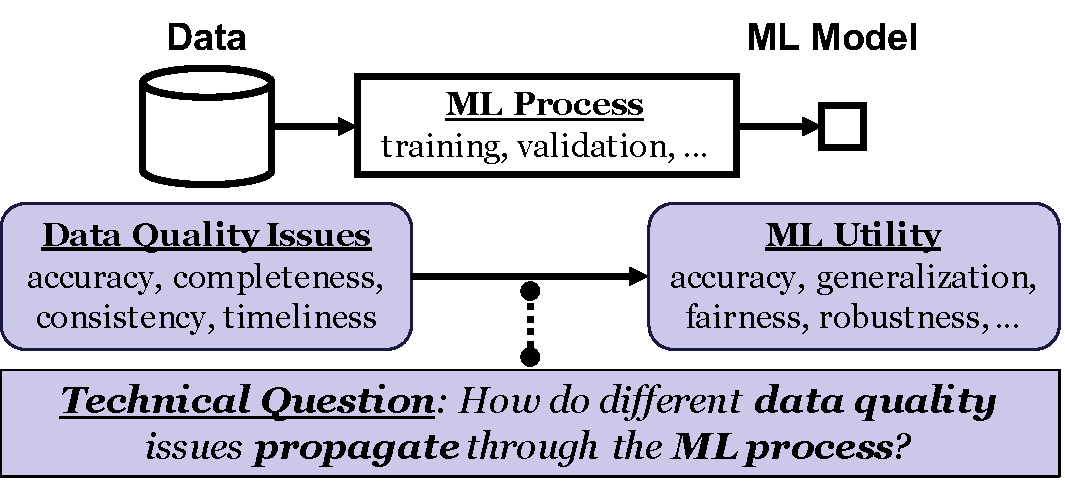
\includegraphics[width=0.5\textwidth]{submissions/data-quality-ml-ops/figs/techq.pdf}
\end{center}
\vspace{-2em}
\vspace{-1em}
\end{wrapfigure}

\vspace{-0.5em}
\paragraph*{Our Experiences and Opinions} 
In this paper, we 
provide a bird's-eye view 
of some of our previous 
works that are related to
enabling different functionalities with respect to MLOps. These works are 
inspired by our experience working hand-in-hand with academic and industrial users to build
ML applications~\cite{schawinski2017generative, su2018generative, sartori2018model, stark2018psfgan, ackermann2018using, schawinski2018exploring, girardi2018patient, glaser2019radiogan, beck2019sensing, sartori2019forward}, together with  
our effort of building 
\texttt{ease.ml}~\cite{aguilar2021ease}, a prototype
system that defines an 
end-to-end MLOps process.

Our key observation is 
that often \textit{
MLOps challenges are bound to
data management challenges} --- 
given the aforementioned 
strong dependency 
between the quality of 
ML models and the quality of data, the never-ending
pursuit of \textit{understanding,
measuring}, and \textit{improving the
quality of ML models},
often hinges on 
\textit{understanding,
measuring}, and \textit{improving
the underlying 
data quality issues}.
From a technical perspective, this poses 
unique challenges and opportunities.
As we will see, we find it necessary to 
revisit decades of 
data quality research
that are agnostic to 
downstream ML models and 
try to 
understand different 
data quality dimensions -- accuracy, completeness,
consistency, and timeliness -- jointly with the downstream ML process. 

In this paper, we describe 
four of such examples, originated from our 
previous research~\cite{karlavs2020nearest, renggli2020automatic, karimi2020online, renggli2019continuous}.
Table~\ref{tbl:overview}
summarizes 
these examples, each of which tackles one
specific problem in MLOps and
poses technical challenges 
of jointly analyzing data quality 
and downstream ML processes.

\begin{table}[t!]
\caption{Overview of 
our explorations with data quality propagation at different stages of an MLOps 
process.}
\label{tbl:overview}
\vspace{-0.5em}
\small
\centering
\begin{tabular}{@{}llll@{}}
\toprule
\textbf{Technical Problem for ML}                           & \textbf{MLOps Stage}         & \textbf{MLOps Question}                                   & \textbf{Data Quality Dimensions}        \\ \midrule
Data Cleaning (Sec.~\ref{sec:cpclean})~\cite{karlavs2020nearest}              & Pre Training  & Which training sample 
to clean?              &
Accuracy \& Completeness\\
Feasibility Study (Sec.~\ref{sec:snoopy})~\cite{renggli2020automatic}         & Pre Training  & Is my target accuracy realistic? & Accuracy \& Completeness\\
CI/CD (Sec.~\ref{sec:ci})~\cite{renggli2019continuous} & Post Training & 
Am I overfitting to val/test? & Timeliness\\
Model Selection (Sec.~\ref{sec:model_picker})~\cite{karimi2020online}        & Post Training & Which samples should I label?                        & Completeness \& Timeliness\\
\bottomrule
\end{tabular}
\end{table}

\vspace{-0.5em}
\paragraph*{Outline}
In Section~\ref{sec:ml} we provide a setup for studying this topic, highlighting the importance of taking the underlying probability distribution into account. In Sections~\ref{sec:cpclean}-\ref{sec:model_picker} we revisit components of different stages of the \texttt{ease.ml} system purely from a data quality perspective. Due to the nature of this paper, we avoid going into the details of the interactions between these components or
their technical details.
Finally, in Section~\ref{sec:limitations} we describe a common limitation that all the components share, and motivate interesting future work in this area.

\section{Machine Learning Preliminaries}
\label{sec:ml}

In order to highlight the strong dependency between the data samples used to train or validate an ML model and its assumed underlying probability distribution, we start by giving a short primer on ML. In this paper we restrict ourselves on supervised learning in which, given a \textit{feature space} $\cX$ and a \textit{label space} $\cY$, a user is given access to a dataset with $n$ samples  $\cD := \{(x_i, y_i)\}_{i \in [n]}$, where $x_i \in \cX$ and $y_i \in \cY$. Usually $\cX \subset \RR^d$, in which case a sample is simply a $d$-dimensional vector, whereas $\cY$ depends on the task at hand. For a regression task one usually takes $\cY = \RR$, whilst for a classification task on $C$ classes one usually assumes $\cY = \{1,2,\ldots,C\}$. We restrict ourselves to classification problems.

Supervised ML aims at \textit{learning} a map $h: \cX \rightarrow \cY$ that generalizes to unseen samples based on the provided labeled dataset $\cD$. 
A common assumption used to learn the mapping is that all data points in $\cD$ are sampled identically and independently (i.i.d.) from an unknown distribution $p(X,Y)$, where $X,Y$ are random variables taking values in $\cX$ and $\cY$, respectively. For a single realisation $(x, y)$, we abbreviate $p(x,y) = p(X\!=\!x,\!Y\!=\!y)$. 

The goal is to choose $h(\cdot) \in \cH$, 
where $\cH$ represents the hypothesis space, that minimizes the expected risk with respect to the underlying probability distribution~\cite{shalev2014understanding}. In other words, one wants to construct $h^*$ such that
\begin{equation}
\label{eq:expected_risk}
h^* = \arg \min_{h \in \cH} \mathbb{E}_{X,Y} \left( L(h(x), y) \right) = \arg \min_{h \in \cH} \int_\cX \int_\cY L(h(x), y) p(x, y)\,dy\,dx ,
\end{equation}
with $L(\hat{y}, y)$ being a loss function that penalizes wrongly predicted labels  $\hat{y}$. For example, $L(\hat{y}, y) = \mathbf{1} (\hat{y} = y)$ represents the 0-1 loss, commonly chosen for classification problems. 
Finding the optimal mapping $h^*$ is not feasible in practice: (1) the underlying probability $p(X,Y)$ is typically unknown and it can only be approximated using a finite number of samples, (2) even if the distribution were known, calculating the integral is intractable for many possible choices of $p(X,Y)$. Therefore, in practice one performs an empirical risk minimization (ERM) by solving 
$\hat{h} = \arg \min_{h \in \cH} \frac{1}{n} \sum_{i=1}^n L(h(x_i), y_i).$
Despite the fact that the model is learned using a finite number of data samples, the ultimate goal is to learn a model which generalizes to any sample originating from the underlying probability distribution, by approximating its posterior $p(Y|X)$.
Using $\hat{h}$ to approximate $h^*$ can run into what-is-known as ``overfitting'' to the training set $\cD$, which reduces the generalization property of the mapping.
However, advances in statistical learning theory managed to considerably lower the expected risk for many real-world applications whilst avoiding overfitting~\cite{friedman2001elements, vapnik2015uniform, shalev2014understanding}.  Altogether, any aspect of data quality for ML application development should not only be treated with respect to the dataset $\cD$ or individual data points therein, but also \emph{with respect to the underlying probability distribution the dataset $\cD$ is sampled from}.

\paragraph{Validation and Test}

Standard ML cookbooks suggest that the data should be represented by three disjoint sets to \emph{train}, \emph{validate}, and \emph{test}. 
The validation set accuracy is typically used to choose the best possible set of hyper-parameters used by the model trained on the training set.
The final accuracy and generalization properties are then evaluated on the test set. Following this, we use the term \textit{validation} for evaluating models in the pre-training phase, and the term \textit{testing} for evaluating models in the post-training phase.

\paragraph{Bayes Error Rate}
Given a probability distribution $p(X,Y)$, the lowest possible error rate achievable by \textit{any} classifier is known in the literature as the Bayes Error Rate (BER). It can be written as
\begin{equation}
\label{eq:bayes_error}
R_{X,Y}^* = \mathbb{E}_{X} \left[ 1- \max_{y\in\cY} p(y| x) \right],
\end{equation}
and the map $h_{opt}(x)=\arg \max_{y\in\cY} p(y \vert x)$ is called the \textit{Bayes Optimal Classifier}. It is important to note that, even though $h_{opt}$ is the best possible classifier (that is often intractable for the reason stated above), its expected risk might still be greater than zero, which results in the accuracy being at most $1 - R_{X,Y}^*$. In Section~\ref{sec:snoopy}, we will outline multiple reasons and provide examples for a non-zero BER.

\paragraph{Concept Shift}

The general idea of ML described so far assumes that the probability distribution $P(X, Y)$ remains fixed over time, which is sometimes not the case in practice~\cite{widmer1996learning, tsymbal2004problem, gama2014survey}. Any change of distribution over time is known as a \textit{concept shift}.
Furthermore, it is often assumed that both the feature space $\cX$ and label space $\cY$ remain identical over a change of distribution, which could also be false in practice. A change of $\cX$ or $p(X)$ (marginalized over $Y$) is often referred to as a \textit{data drift}, which can result in missing values for training or evaluating a model. We will cover this specific aspect in Section~\ref{sec:cpclean}. When a change in $p(X)$ modifies $p(Y\vert X)$, this is known as a \textit{real drift} or a \textit{model drift}, whereas when $p(Y\vert X)$ stays intact it is a \textit{virtual drift}. Fortunately, virtual drifts have little to no impact on the trained ML model, assuming one managed to successfully approximate the posterior probability distribution over the entire feature space $\cX$.

\section{MLOps Task 1: Effective ML Quality Optimization}
\label{sec:cpclean}

\begin{figure}[t!]
\centering
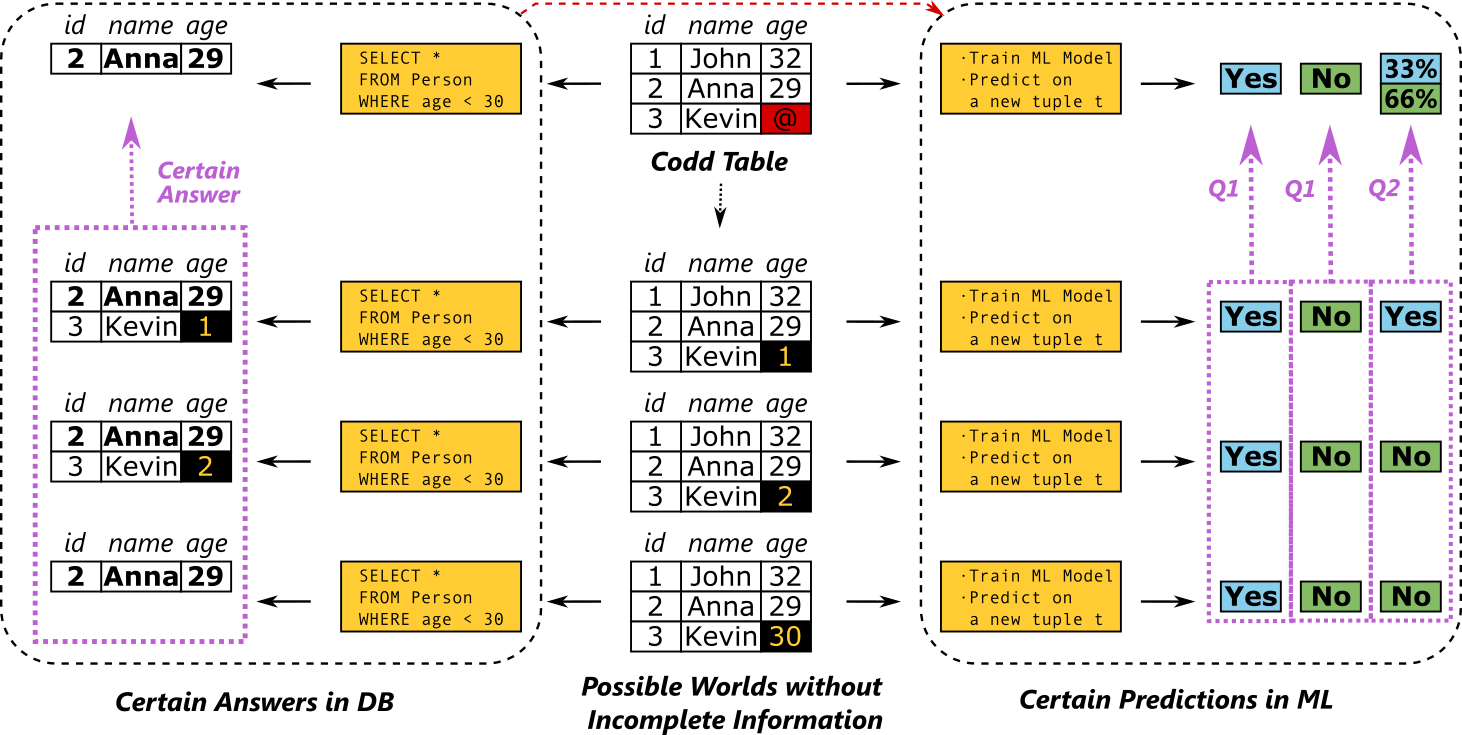
\includegraphics[width=0.9\textwidth]{submissions/data-quality-ml-ops/figs/cpclean.png}
\caption{Illustration of the relation between Certain Answers and Certain Predictions~\cite{karlavs2020nearest}. On the right, Q1 represents a \textit{checking query}, whereas Q2 is a \textit{counting query}.}
\label{fig:cpclean}
\end{figure}


\vspace{-0.5em}
One key operation in MLOps is seeking a way to 
improve the quality (e.g., accuracy) of a model.
Apart from trying new architectures and models,
improving the quality and quantity of the training
data has been known to be at least as important~\cite{li2019cleanml,fernandez2014we}.
Among many other approaches, data cleaning~\cite{ilyas2019data}, the practice of fixing 
or removing noisy and dirty samples,
has been a well-known strategy for improving 
the quality of data.

\vspace{-0.5em}
\paragraph*{MLOps Challenge}
When it comes to MLOps, a challenge is that 
not all noisy or dirty samples matter equally 
to the quality of the final ML model. In other words --
when ``propagating'' through the ML training process,
noise and uncertainty of different input samples
might have vastly different effects. As a result,
simply cleaning the input data artifacts either
randomly or agnostic to the ML 
training process might lead to a sub-optimal improvement
of the downstream ML model~\cite{li2019cleanml}.
Since the cleaning task itself is often 
performed ``semi-automatically'' 
by human annotators, with guidance from automatic
tools, the goal of a \textit{successful} cleaning strategy from an MLOps perspective should be to minimize the amount of human effort. This typically leads to a partially cleaned dataset, with the property that cleaning additional training samples would not affect the outcome of the trained model (i.e., the predictions and accuracy on a validation set are maintained).

 \vspace{-0.5em}
\paragraph*{A Data Quality View}
A principled solution to the above 
challenge requires a \textit{joint}
analysis of the impact of incomplete and noisy data in the training
set on the quality of an ML model trained over
such a set. Multiple seminal works have studied this problem, e.g., ActiveClean~\cite{krishnan2016activeclean}.
Inspired by these, we introduced 
a principled framework called CPClean that models
and analyzes such a 
noise propagation process together with principled cleaning algorithms based on 
sequential information maximization~\cite{karlavs2020nearest}.

\paragraph{Our Approach: Cleaning with CPClean}
CPClean directly models the noise propagation ---
the noises and incompleteness introduce
multiple possible datasets, called \emph{possible worlds} in relational database theory,
and the impact of these noises to 
final ML training is simply the \textit{entropy} 
of training multiple ML models, one for each of these possible worlds. Intuitively,
the smaller the entropy, the less impactful
the input noise is to the downstream 
ML training process.
Following this, we start by initiating all possible worlds (i.e., possible versions of the training data after cleaning) by applying multiple well-established cleaning rules and algorithms independently over missing feature values.
CPClean then operates in multiple iterations. At each round, the framework suggests the training data to clean that minimizes the \textit{conditional entropy} of possible worlds over the partially clean dataset. Once a training data sample is cleaned, it is replaced by its cleaned-up version in all possible worlds. At its core, it uses a \emph{sequential information-maximization} algorithm that finds an approximate solution (to this NP-Hard problem) with theoretical guarantees~\cite{karlavs2020nearest}.
Calculating such an entropy is often difficult,
whereas in CPClean we provide efficient algorithms which can calculate this term in polynomial time for a specific family of 
classifiers, namely k-nearest-neighbour
classifiers (kNN).

This notion of learning over incomplete data using \emph{certain predictions} is inspired by research on \emph{certain answers} over incomplete data~\cite{abiteboul1995foundations, suciu2011probabilistic, arenas1999consistent}. In a nutshell, the latter reasons about \emph{certainty} or \emph{consistency} of the answer to a given input, which consists of a query and an incomplete dataset, by enumerating the results over all possible worlds. Extending this view of data incompleteness to non-relational operator (e.g., an ML model) is a natural yet non-trivial endeavor, and Figure~\ref{fig:cpclean} illustrates the connection.

\paragraph{Limitations}
Taking the downstream ML model into account for prioritizing human cleaning effort is not new. ActiveClean~\cite{krishnan2016activeclean} suggests to use information about the \textit{gradient} of a fixed model to solve this task. Alternatively, our framework relies on consistent predictions and, thus, works on an unlabeled validation set
and on ML models that are not differentiable. 
In~\cite{karlavs2020nearest}
we use kNN as a proxy to an arbitrary classifier, given its efficient implementation despite exponentially many possible worlds. However, it still remains to be seen
how to extend this principled framework 
to other types of classifiers. Moreover, combining both approaches and supporting a labor-efficient cleaning approach for general ML models remains an open research problem.

\section{MLOps Task 2: Preventing Unrealistic Expectations}
\label{sec:snoopy}

In DevOps practices, new projects are typically initiated with a \textit{feasibility study}, in order to evaluate and understand the probability of success. The goal of such a study is to prevent users with unrealistic expectations from spending a lot of of money and time on developing solutions that are doomed to fail. However, when it
comes to MLOps practices, such a 
feasibility study step is largely missing --- we often
see users with high expectations, but with a very noisy dataset, starting an
expensive training process which is almost surely
doomed to fail.


\paragraph*{MLOps Challenge}
One principled way to model the feasibility
study problem for ML is to ask:
\textit{Given an ML task, defined by its training and validation sets, how to estimate the 
error that the best
possible ML model can achieve, without
running expensive ML training?}
The answer to this question 
is linked to a traditional ML problem, i.e.,
to estimate the \emph{Bayes error rate} (also called \emph{irreducible error}). It is a quantity related to the underlying data distribution and estimating it using finite amount of data is known to be a notoriously hard problem. Despite decades of study~\cite{cover1967nearest, fukunaga1987bayes, sekeh2018multi},
providing a practical BER estimator is still 
an open research problem and there are no known practical 
systems that can work on real-world large-scale datasets. One key challenge to make feasibility
study a practical MLOps step is to understand 
how to utilize decades of theoretical studies
on the BER estimation and which  
compromises and optimizations to perform.


\begin{figure}[t!]
%\begin{subfigure}[t]{.32\textwidth}
\begin{subfigure}%{\linewidth}
\centering%\captionsetup{width=.3\textwidth}
%\label{fig:imnet_missingfeature}
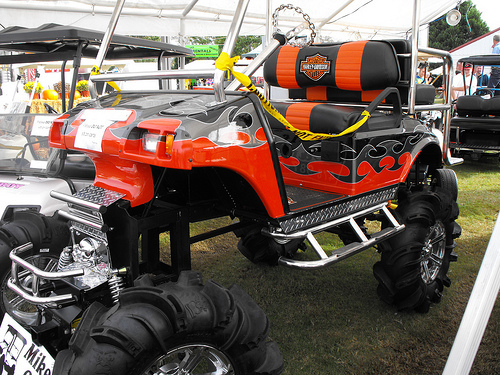
\includegraphics[width=0.3\textwidth]{submissions/data-quality-ml-ops/figs/ILSVRC2012_val_00006874.JPEG}  
%\caption{}
\end{subfigure}
\hfill
\begin{subfigure}%{\linewidth}
\centering%\captionsetup{width=.3\textwidth}
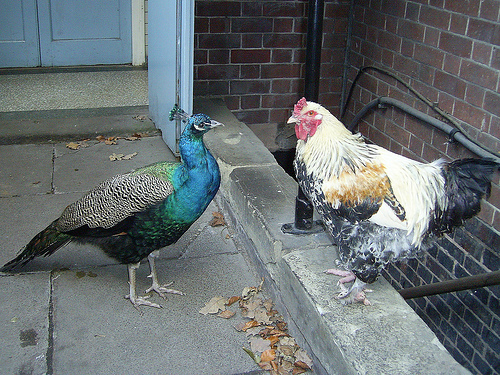
\includegraphics[width=0.3\textwidth]{submissions/data-quality-ml-ops/figs/ILSVRC2012_val_00004463.JPEG}  
%\caption{Image (\#4463) showing multiple classes for a fixed sample.}
%\label{fig:imnet_missinglabel}
\end{subfigure}
\hfill
\begin{subfigure}%{.32\linewidth}
\centering%\captionsetup{width=.3\textwidth}
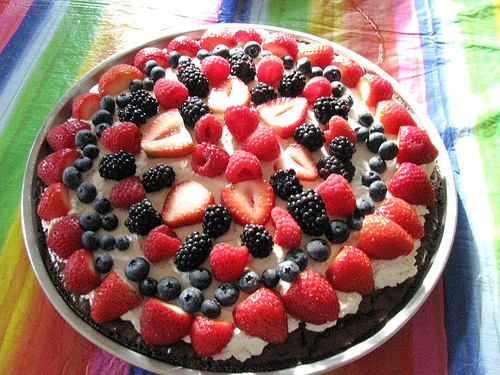
\includegraphics[width=0.3\textwidth]{submissions/data-quality-ml-ops/figs/ILSVRC2012_val_00032040.JPEG}  
%\caption{Image (\#32040) mislabeled as a ``pizza''.}
%\label{fig:imnet_labelnoise}
\end{subfigure}
\caption{ImageNet examples from the validation set illustrating possible reasons for a non-zero Bayes Error. Image (\#6874) on the left illustrates a non-unique label probability, image (\#4463) in the middle shows multiple classes for a fixed sample, and image (\#32040) on the right is mislabeled as a ``pizza''.}
\label{fig:imagenet_examples}
\end{figure}

\subparagraph{Non-Zero Bayes Error and Data Quality Issues}
At the first glance, even understanding why the BER is not zero for every task can be quite mysterious --- 
\textit{if we have enough amount of data and 
a powerful ML model, what would stop us from 
achieving perfect accuracy?}
The answer to this is deeply connected to 
data quality.
There are two classical data quality dimensions that constitute the reasons for a non-zero BER: (1)~\textit{completeness} of the data, violated by an insufficient definition of either the feature space or label space, and (2)~\textit{accuracy} of the data, mirrored in the amount of noisy labels. 
On a purely mathematical level, the reason for a non-zero BER lies in \textit{overlapping} posterior probabilities for different classes, given a realisable input feature.
More intuitively, for a given sample the label might not be unique.
In Figure~\ref{fig:imagenet_examples} we illustrate some real-world examples from the validation set of \textit{ImageNet}~\cite{deng2009imagenet}.
For instance, the image on the left is labeled as a golfcart (n03445924) 
whereas there is a non-zero probability that the vehicle belongs to another category, for instance a tractor (n04465501) -- additional features can resolve such an issue by providing more information and thus leading to a single possible label.
Alternatively, there might in fact be multiple ``true'' labels for a given image. The center image shows such an example, where the posterior of class rooster (n01514668) is equal to the posterior of the class peacock (n01806143), despite being only labeled as a rooster in the dataset -- changing the task to a multi-label problem would resolve this issue.
Finally, having noisy labels in the validation set yields another sufficient condition for a non-zero BER.
The image on the left shows such an example, where a pie is incorrectly labeled as a pizza (n07873807).

\paragraph*{A Data Quality View}
There are two main challenges in building 
a practical BER estimator for ML models to
characterize the impact of data quality to 
downstream ML models: (1) the computational requirements and (2) the choice of hyper-parameters. Having to estimate the BER in today's high-dimensional feature spaces
requires a large amount of data in order to give a reasonable estimate in terms of accuracy, which results in a high computational cost. Furthermore, any practical estimator should be insensitive to different hyper-parameters, as no information about the data or its underlying distribution is known \emph{prior to} running the feasibility study.

\begin{wrapfigure}{r}{0.5\textwidth}
\vspace{-2em}
\centering
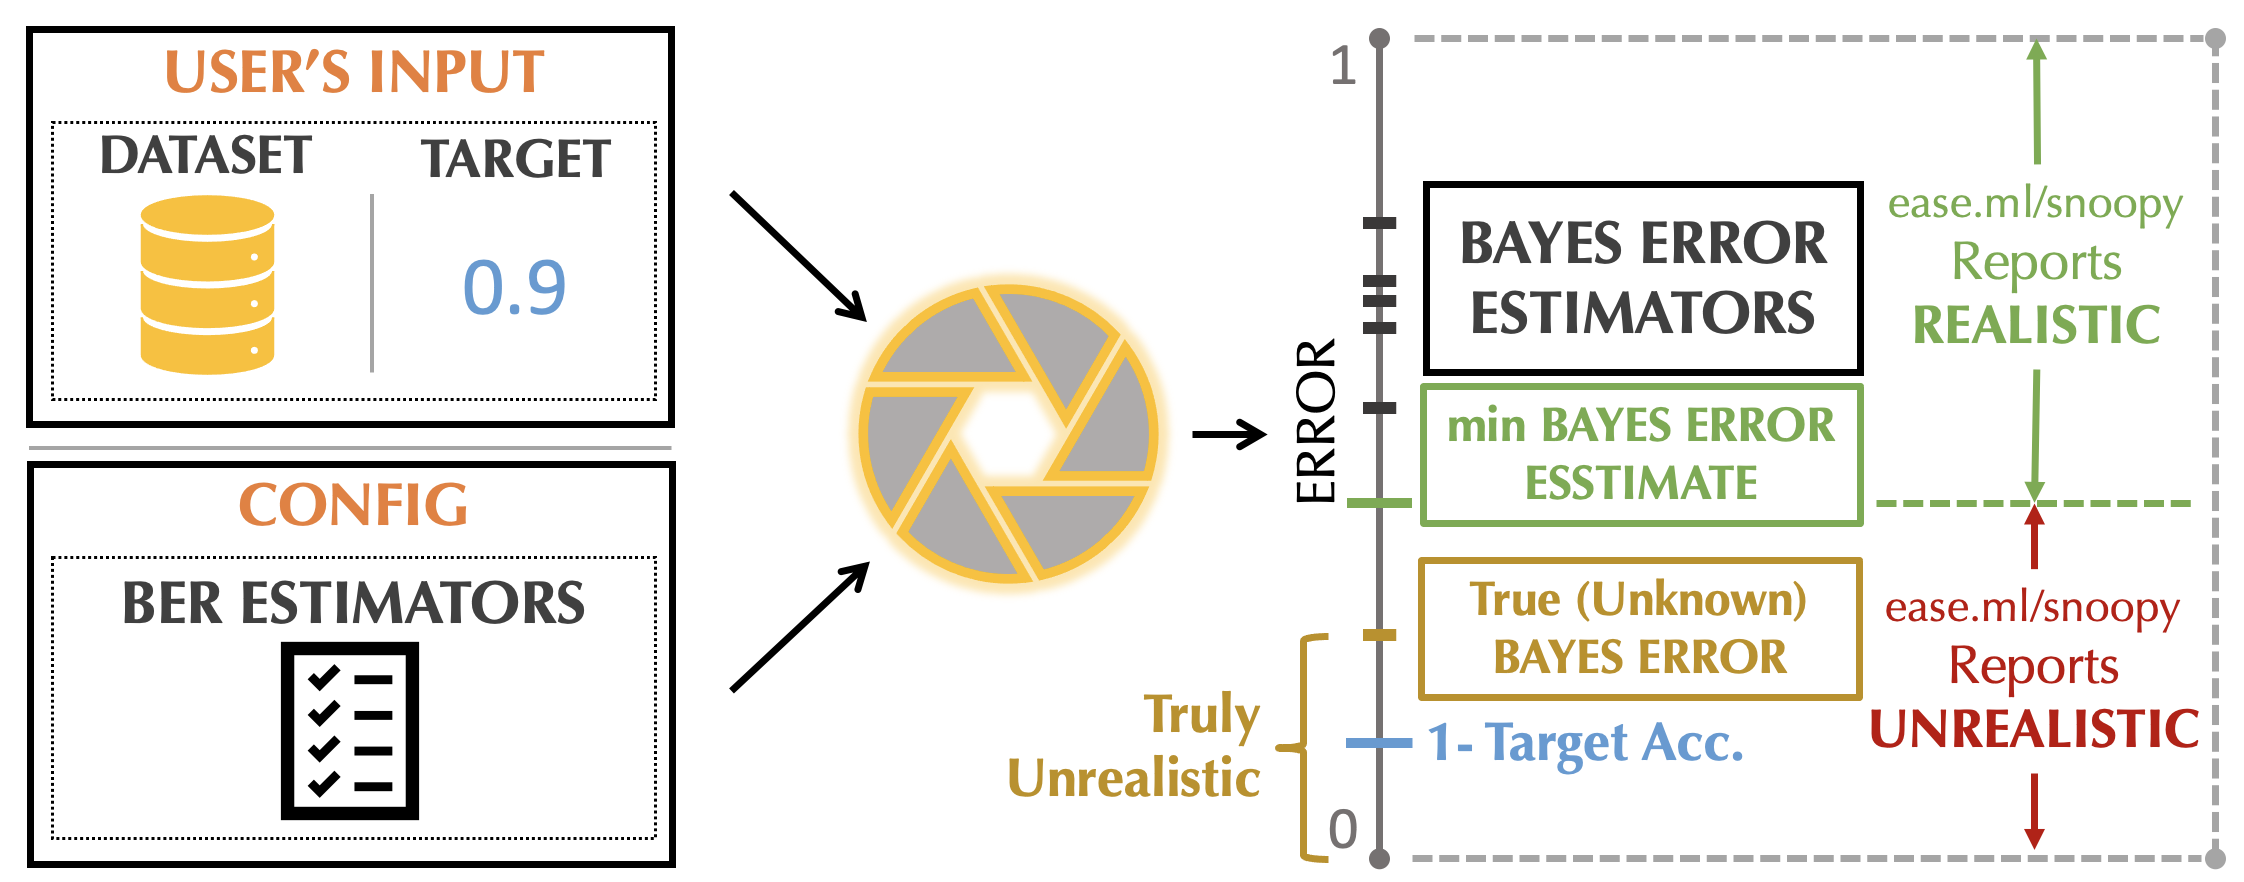
\includegraphics[width=0.5\textwidth]{submissions/data-quality-ml-ops/figs/snoopy.png}
\label{fig:snoopy}
\vspace{-2em}
\end{wrapfigure}

\paragraph{Our Approach: \texttt{ease.ml/snoopy}}
We design a novel BER estimation method that (1) has no hyper-parameters to tune, as it is based on nearest-neighbor estimators, which are non-parametric; and (2) uses pre-trained embeddings, from public sources such as PyTorch Hub or Tensorflow Hub\footnote{\url{https://pytorch.org/hub} and \url{https://tfhub.dev}}, to considerably decrease the dimension of the feature space. The aforementioned functionality of performing a feasibility study using \texttt{ease.ml/snoopy} is illustrated in the above figure. For more details we refer interested readers to both the full paper~\cite{renggli2020automatic} and the demo paper for this component~\cite{renggli2020ease}. The usefulness and practicality of this novel approach is evaluated on well-studied standard ML benchmarks through a new evaluation methodology that injects label noise of various amounts and follows the evolution of the BER~\cite{renggli2020automatic}. It relies on our theoretical work~\cite{rimanic2020convergence}, in which we furthermore provide an in-depth explanation for the behavior of kNN over (possibly pre-trained) feature transformations by showing a clear trade-off between the increase of the BER and the boost in convergence speed that a transformation can yield.


\paragraph{Limitations}
The standard definition of the BER assumes that both the training and validation data are drawn i.i.d. from the \textit{same} distribution, an assumption that does not always hold in practice.
Extending our work to a setup that takes into account two different distributions for training and validation data, for instance as a direct consequence of applying data programming or weak supervision techniques~\cite{ratner2017snorkel}, offers an interesting line of future research, together with developing even more practical 
BER estimators for the i.i.d. case.


\section{MLOps Task 3: Rigorous Model Testing Against Overfitting}
\label{sec:ci}

One of the major advances in running fast and robust cycles in the software development process is known as continuous integration (CI)~\cite{duvall2007continuous}. The core idea is to carefully define and run a set of conditions in the form of tests that the software needs to successfully pass every time prior to being pushed into production. This ensures the robustness of the system and prevents unexpected failures of production code even when being updated.
However, when it comes to MLOps, the traditional 
way of reusing the same test cases repeatedly can 
introduce serious risk of overfitting, thus 
compromise the test result.

\paragraph*{MLOps Challenge}
In order to generalize to the unknown underlying probability distribution, when training an ML model, one has to be careful not to overfit to the (finite) training dataset. However, much less attention has been devoted to the statistical generalization properties of the \textit{test set}.
Following best ML practices, the ultimate testing phase of a new ML model should either be executed only once per test set, or has to be completely obfuscated from the developer. Handling the test set in one way or the other ensures that no information of the test set is \emph{leaked} to the developer, hence preventing potential overfitting. Unfortunately, in ML development environments it is often impractical to implement either of these two approaches.

\paragraph*{A Data Quality View}
Adopting the idea of continuously testing and integrating ML models in productions has two major caveats: (1) test results are inherently random, due to the nature of ML tasks and models, and (2) revealing the outcome of a test to the developer could mislead them into overfitting towards the test set.
The first aspect can be tackled by using well-established concentration bounds known from the theory of statistics.
To deal with the second aspect, which we refer to as the \textit{timeliness} property of testing data, there is an approach pioneered by Ladder~\cite{blum2015ladder}, together with the general area of \emph{adaptive analytics} (cf.~\cite{dwork2015reusable}), that enable multiple reuses of the same test set with feedback to the developers. The key insight of this line of work is that the \textit{statistical power} of a fixed dataset shrinks when increasing the number of times it is reused. In other words, requiring a minimum statistically-sound confidence in the generalization properties of a finite dataset limits the number of times that it can be reused in practice.

\paragraph{Our Approach: Continuous Integration of ML Models with \texttt{ease.ml/ci}}

\begin{figure}
\centering
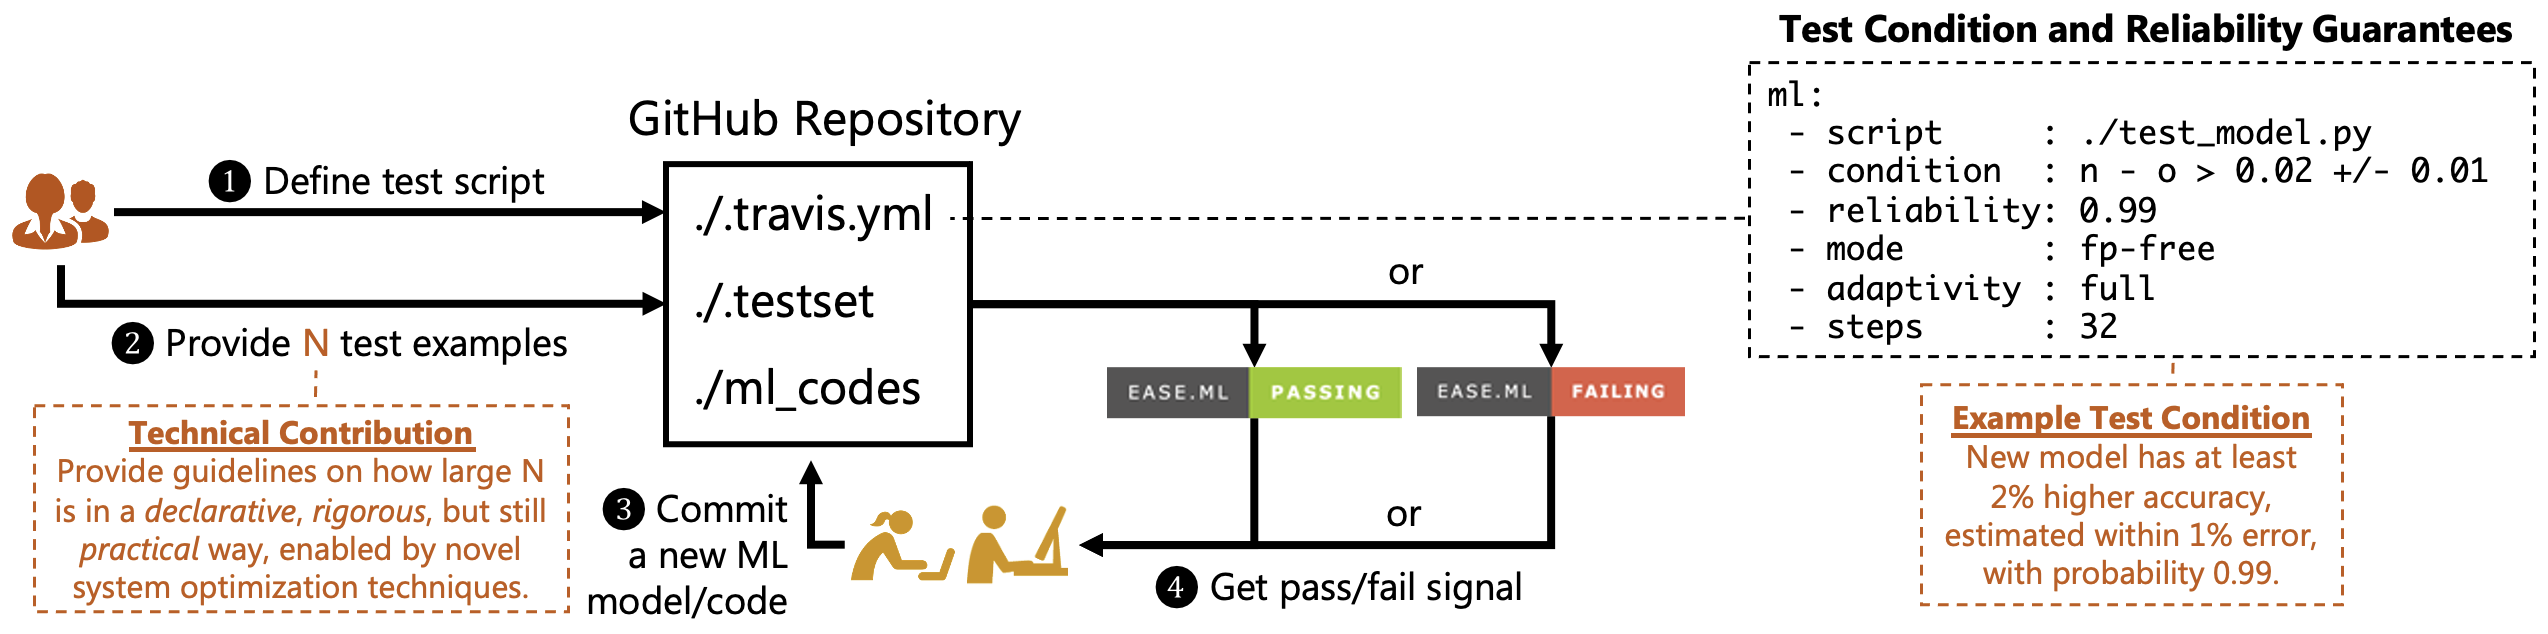
\includegraphics[width=1.0\textwidth]{submissions/data-quality-ml-ops/figs/ci.png}
\caption{The workflow of \texttt{ease.ml/ci}, our CI/CD engine for ML models~\cite{renggli2019continuous}.}
\label{fig:ci}
\end{figure}

As part of the \texttt{ease.ml} pipeline, we designed a CI engine to address both aforementioned challenges. The workflow of the system is summarized in Figure~\ref{fig:ci}. The key ingredients of our system lie in (a) the syntax and semantics of the test conditions and how to accurately evaluate them, and (b) an optimized \emph{sample-size estimator} that yields a budget of test set re-uses before it needs to be refreshed. For a full description of the workflow as well as advanced system optimizations deployed in our engine, we refer the reader to our initial paper~\cite{renggli2019continuous} and the followup work~\cite{karlavs2020building}, which further discusses the integration into existing software development ecosystems.

We next outline the key technical details falling under the 
general area of ensuring generalization properties of finite data used to test the accuracy of a trained ML model repetitively.

\subparagraph{Test Condition Specifications}

A key difference between classical CI test conditions and testing ML models lies in the fact that the test outcome of any CI for ML engine is inherently probabilistic. Therefore, when evaluating result of a test condition that we call a \textit{score}, one has to define the desired confidence level and tolerance as an $(\epsilon,\delta)$ requirement. Here $\epsilon$ (e.g., $1\%$) indicates the size of the confidence interval in which the estimated score has to lie with probability at least $1-\delta$ (e.g., $99\%$). For instance, the condition \verb|n - o > 0.02 +/- 0.01| requires that the new model is at least 2 points better in accuracy than the old one, with a confidence interval of 1 point. Our system additionally supports the variable \verb|d| that captures the fraction of different predictions between the new and old model.  
For testing whether a test condition passes or fails one needs to distinguish two scenarios. On one hand, if the score lies outside the confidence interval (e.g., \verb|n - o > 0.03| or \verb|n - o < 0.01|), the test immediately passes or fails.
On the other hand, the outcome is ill-defined if the score lies inside the confidence interval. Depending on the task, user can choose to allow \emph{false positive} or \emph{false negative} results (also known as ``type I'' and ``type II'' errors 
in statistical hypothesis testing), after which all the scores lying inside the confidence interval will be automatically rejected or accepted.


\subparagraph{Test Set Re-Uses}

In the case of a non-adaptive scenario in which no information is revealed to the developer after running the test, the least amount of samples needed to perform $H$ evaluations with the same dataset is the same as running a single evaluation with $\delta / H$ error probability, since the $H$ models are independent.
Therefore, revealing any kind of information to the developer would result in a dataset of size $H$ multiplied by the number of samples required for one evaluation with $\delta / H$ error. However, this trivial strategy is very costly and usually impractical. The general design of our system offers a different approach that significantly reduces the amount of test samples needed for using the same test set multiple times. More precisely, after every commit the system only reveals a binary pass/fail signal to the developer. Therefore, there are $2^H$ different possible sequences of pass/fail responses, 
which yields that the number of samples needed for $H$ iterations is the same as running a single iteration with $\delta / 2^H$ error probability -- much smaller than the previous $\delta / H$ one. 
We remark that further optimizations can be deployed by making use of the structure or low variance properties that are present in certain test conditions, for which we refer the interested readers to the full paper~\cite{renggli2019continuous}.

\paragraph{Limitations}

The main limitation consists of the worst-case analysis which happens when the developer acts as an adversarial player that aims to overfit towards the hidden test set. Pursuing other, less pragmatic approaches to model the behavior of developers could enable further optimization to reduce the number of test samples needed in this case.
A second limitation lies in the lack of ability to handle concept shifts. Monitoring a concept shift could be thought of as a similar process of CI -- instead of fixing the test set and testing multiple models, one could fix a single model and test its generalization over multiple test sets. From that perspective, we hope that some of the optimizations that we have derived in our work could potentially be applied to monitoring concept shifts as well. Nevertheless, this needs further study and forms an interesting research path for the future.

%\newpage
\section{MLOps Task 4: Efficient Continuous Quality Testing}
\label{sec:model_picker}

One of the key motivations for DevOps principles in the first place is the ability to perform fast cycles and continuously ensure the robustness of a system by quickly adapting to changes. At the same time, both are well-known requirements from traditional software development that naturally extend to the MLOps world.
One challenge faced by many MLOps practitioners is the necessity
to deal with the shift of data distributions when models are
in production. When new production 
data comes from a different (unknown) distribution,
models trained over previously seen 
data distributions might not perform well
anymore. 

\paragraph*{MLOps Challenge}
While there has been various research on 
automatic domain adaption~\cite{shimodaira2000improving, sugiyama2008direct, zhang2013domain}, we identify a 
different challenge when presented with a collection of models, each of which could be a ``staled model'' or 
an automatically adapted model given some domain adaption method. 
This scenario is quite common in many 
companies --- they often train distinct models on
different slices of data independently (for instance one model for each season) and 
automatically adapt each of these
models using different methods for new data. As a result,
they often have access to a large 
set of models that could be deployed, hoping to know which one to use given
a fresh collection of production data (e.g., the current time period such as the current day).
The challenge is, given an unlabeled 
production data stream, to pick the model that
performs best. From the MLOps perspective,
the goal is to minimize the amount of labels needed to 
acquire in order to make such a distinction. 


\paragraph*{A Data Quality View}
Concept shift is by its definition related to the \textit{timeliness} properties of the data. The available pre-trained models are intended to capture the changes of training data over time. Naturally, simple rules can be applied to choose the current model if one has access to some meta information about both the current timestamp and the pre-trained models (e.g., the current weekday and for each model the day it represents).
This problem gets particularly difficult when there are no such meta-data available. In that case, having access to a fully labeled clean dataset would result in trivially selecting the pre-trained model that achieves the highest accuracy. Collecting labels for a large enough test set is very costly in practice compared to simply gathering a set of unlabeled samples though. The reason is that accurately labeling samples requires human, if not expert level, annotators. Consequently, one wishes to robustly solve the problem of \textit{picking} the best model for the current time span with the fewest amount of labeling effort necessary and thus relying on \textit{incomplete} test data with respect to their labels.

\paragraph{Our Approach: \texttt{ease.ml/ModelPicker}}
Model Picker is an online model selection approach to selectively sample instances that are informative for ranking pre-trained models~\cite{karimi2020online}. Specifically, given a set of pre-trained models and a stream of unlabeled data samples that arrive sequentially from a data source, the Model Picker algorithm answers when to query the label of an instance, in order to pick the best model under limited labeling budget. We conduct a rigorous theoretical analysis to show that Model Picker has no regret for adversarial streams (e.g., non-i.i.d. data), and is effective in online prediction tasks for both adversarial and stochastic streams. Moreover, our theoretical bounds match (up to constants) those of existing online algorithms that have access to all the labels. 

\paragraph{Limitations}
One immediate extension of Model Picker is towards a setting in which the user at once has access to a pool of unlabeled data samples. In such a \textit{pool-based sampling} case~\cite{settles2009active}, one can rank the entire collection of data samples to select the most informative example instead of scanning through the data sequentially to decide whether to query a label or not. Despite the applicability of Model Picker to such a scenario where one can form a stream by sampling i.i.d. from the pool of samples, the availability of entire data collection can be exploited to further reduce the annotation costs with a more specialized strategy for pool-based scenarios.

%\newpage
\section{Moving Forward}
\label{sec:limitations}

We have briefly described four 
of our previous works with a unified theme ---
all of them provide, in our opinion, \textit{
functionalities that are useful to 
facilitate a better MLOps process}, which, on 
the flip side, introduce new fundamental 
technical problems that require us to 
\textit{jointly analyze the impact
of data quality issues to downstream ML processes.}
When studying these technical problems,
we often need to 
go beyond an ML-agnostic view 
of data quality and, instead, need to develop 
new methods that \emph{simultaneously} combine the two aspects of ML \emph{and} data quality.
Despite the progress that we have made so far, this endeavor is still at its early stages. 
In the following, we present two future directions that, in our opinion,
are necessary to facilitate both MLOps as an important
functionality and ML-aware data quality as a fundamental research area.


\paragraph*{ML-Aware Data Quality}
From a technical perspective,
jointly understanding data quality and 
downstream ML processes is both interesting
and challenging. All results we discussed
in this paper are arguably limited~\cite{karlavs2020nearest, renggli2020automatic, karimi2020online, renggli2019continuous} --- after starting 
from a principled formulation of a 
problem, reaching fundamental 
computational challenges within these  
principled frameworks is inevitable. We get around
those by either (1) opting for simpler 
proxy models for which we can derive 
stronger results and/or more efficient algorithms
(e.g., kNN used in \texttt{ease.ml/snoopy}~\cite{renggli2020automatic}
and CPClean~\cite{karlavs2020nearest})
or (2) optimizing for specific cases 
commonly used in practice (e.g., the patterns in \texttt{ease.ml/ci}~\cite{renggli2019continuous} that we optimized for).
To further facilitate MLOps in general,
we are in dire need for an 
ML-aware data quality that is not only principled,
but also practical for a larger 
collection of scenarios and ML models.
These are all technically challenging --- simply
extending the methods that we developed is unlikely to succeed.
We hope that our current endeavors~\cite{karlavs2020nearest, renggli2020automatic, karimi2020online, renggli2019continuous} can serve, in
some ways, as ``examples of failures''
that other researchers can draw inspirations from.

\paragraph{Beyond Accuracy}
Another common limitation of our work~\cite{karlavs2020nearest, renggli2020automatic, karimi2020online, renggli2019continuous}
is that they all focus on improving the \textit{accuracy} of an ML model artifact. Although this is one of the most important 
aspects of model quality, recently researchers have
also identified multiple interesting dimensions
of model quality such as robustness, fairness,
and explainability. 
Even though we expect these quality dimensions to
become the core of the MLOps process in the future,
how to extend functionalities that we 
developed for improving accuracy to 
these quality dimensions is still an open question.
Jointly analyzing the impact of all data-quality dimensions with respect to more than a single metric that quantifies ML models is a large and promising research area that we believe will provide further understanding and improvements of the MLOps process.


\section*{Acknowledgments}
\small
We are grateful to many collaborators that we have 
been working with over the years, especially (in the context of this paper) those
who also contributed to the development of techniques in \cite{karlavs2020nearest, renggli2020automatic, karimi2020online, renggli2019continuous} including Peng Li, Prof. Xu Chu, Mohammad Reza Karimi, and Prof. Andreas Krause. These technical results would not be possible without their contributions.

CZ and the DS3Lab gratefully acknowledge the support from the Swiss National Science Foundation (Project Number 200021\_184628), Innosuisse/SNF BRIDGE Discovery (Project Number 40B2-0\_187132), European Union Horizon 2020 Research and Innovation Programme (DAPHNE, 957407), Botnar Research Centre for Child Health, Swiss Data Science Center, Alibaba, Cisco, eBay, Google Focused Research Awards, Oracle Labs, Swisscom, Zurich Insurance, Chinese Scholarship Council, and the Department of Computer Science at ETH Zurich.

\newpage
\bibliographystyle{abbrv}
\bibliography{submissions/data-quality-ml-ops/ieeedeb}

\end{document}
\end{article}

\begin{article}
{From Cleaning before ML to Cleaning for ML}
{Felix Neutatz, Binger Chen, Ziawasch Abedjan and Eugene Wu}
\pdfminorversion=5
\documentclass[11pt]{article}
\usepackage{deauthor,times,graphicx,caption,microtype}
\usepackage{hyperref}
\usepackage{listings}
\usepackage{booktabs}

\begin{document}

\title{Optimistic Lock Coupling: A Scalable and Efficient General-Purpose Synchronization Method}

\author{Viktor Leis, Michael Haubenschild\raisebox{0.9ex}{$\ast$}, Thomas Neumann\\ Technische Universit{\"a}t M{\"u}nchen \hspace{0.7cm} Tableau Software\raisebox{0.9ex}{$\ast$} \\ {\{leis,neumann\}{@}in.tum.de} \hspace{0.7cm} {mhaubenschild{@}tableau.com\raisebox{0.9ex}{$\ast$}}}

\maketitle

\begin{abstract}
As the number of cores on commodity processors continues to increase, scalability becomes more and more crucial for overall performance.
Scalable and efficient concurrent data structures are particularly important, as these are often the building blocks of parallel algorithms.
Unfortunately, traditional synchronization techniques based on fine-grained locking have been shown to be unscalable on modern multi-core CPUs.
Lock-free data structures, on the other hand, are extremely difficult to design and often incur significant overhead.

In this work, we make the case for Optimistic Lock Coupling as a practical alternative to both traditional locking and the lock-free approach.
We show that Optimistic Lock Coupling is highly scalable and almost as simple to implement as traditional lock coupling.
Another important advantage is that it is easily applicable to most tree-like data structures.
We therefore argue that Optimistic Lock Coupling, rather than a complex and error-prone custom synchronization protocol, should be the default choice for performance-critical data structures.
\end{abstract}

\section{Introduction}

% more and more cores
Today, Intel's commodity server processors have up to 28 cores and its upcoming microarchitecture will have up to 48 cores per socket~\cite{intel}.
Similarly, AMD currently stands at 32 cores and this number is expected to double in the next generation~\cite{amd}.
Since both platforms support simultaneous multithreading (also known as hyperthreading), affordable commodity servers (with up to two sockets) will soon routinely have between 100 and 200 hardware threads.

% data structure scalability is important
With such a high degree of hardware parallelism, efficient data processing crucially depends on how well concurrent data structures scale.
Internally, database systems use a plethora of data structures like table heaps, internal work queues, and, most importantly, index structures.
Any of these can easily become a scalability (and therefore overall performance) bottleneck on many-core CPUs.

% traditional synchronization: fine-grained locks, slow, cache invalidation
Traditionally, database systems synchronize internal data structures using fine-grained reader/writer locks\footnote{In this work, we focus on data structure synchronization rather than high-level transaction semantics and therefore use the term {\em lock} for what would typically be called {\em latch} in the database literature. We thus follow common computer science (rather than database) terminology.}.
Unfortunately, while fine-grained locking makes lock contention unlikely, it still results in bad scalability because lock acquisition and release require writing to shared memory.
Due to the way cache coherency is implemented on modern multi-core CPUs, these writes cause additional cache misses\footnote{The cache coherency protocol ensures that all copies of a cache line on other cores are invalidated before the write can proceed.} and the cache line containing the lock's internal data becomes a point of physical contention.
As a result, any frequently-accessed lock (e.g., the lock of the root node of a B-tree) severely limits scalability.

% lock-free bw-tree: no more latches, but indirections, extremely complex
Lock-free data structures like the Bw-tree~\cite{DBLP:conf/icde/LevandoskiLS13a} (a lock-free B-tree variant) or the Split-Ordered List~\cite{DBLP:journals/jacm/ShalevS06} (a lock-free hash table) do not acquire any locks and therefore generally scale much better than locking-based approaches (in particular for read-mostly workloads).
However, lock-free synchronization has other downsides:
First, it is very difficult and results in extremely complex and error-prone code (when compared to locking).
Second, because the functionality of atomic primitives provided by the hardware (e.g., atomically compare-and-swap 8 bytes) is limited, complex operations require additional indirections within the data structure.
For example, the Bw-tree requires an indirection table and the Split-Ordered List requires ``dummy nodes'', resulting in overhead due to additional cache misses.

% OLC for the win
In this paper we make the case for {\em Optimistic Lock Coupling (OLC)}, a synchronization method that combines some of the best properties of lock-based and lock-free synchronization.
OLC utilizes a special lock type that can be used in two modes:
The first mode is similar to a traditional mutex and excludes other threads by physically acquiring the underlying lock.
In the second mode, reads can proceed optimistically by validating a version counter that is embedded in the lock (similar to optimistic concurrency control).
The first mode is typically used by writers and the second mode by readers.
Besides this special lock type, OLC is based on the observation that optimistic lock validations can be interleaved/coupled---similar to the pair-wise interleaved lock acquisition of traditional lock coupling.
Hence, the name Optimistic Lock Coupling.

OLC has a number of desirable features:
\begin{itemize}
\item By reducing the number of writes to shared memory locations and thereby avoiding cache invalidations, it {\bf scales well} for most workloads.
\item In comparison to unsynchronized code, it requires few additional CPU instructions making it {\bf efficient}.
\item OLC is {\bf widely applicable} to different data structures. It has already been successfully used for synchronizing binary search trees~\cite{DBLP:conf/ppopp/BronsonCCO10}, tries~\cite{artsync}, trie/B-tree hybrids~\cite{DBLP:dblp_conf/eurosys/MaoKM12}, and B-trees~\cite{buzzword}.
\item In comparison to the lock-free paradigm, it is also {\bf easy to use} and requires few modifications to existing, single-threaded data structures.
\end{itemize}
Despite these positive features and its simplicity, OLC is not yet widely known.
The goal of this paper is therefore to popularize this simple idea and to make a case for it.
We argue that OLC deserves to be widely known.
It is a good default synchronization paradigm---more complex, data structure-specific protocols are seldom beneficial.

The rest of the paper is organized as follows.
Section~\ref{sec:related} discusses related work, tracing the history of OLC and its underlying ideas in the literature.
The core of the paper is Section~\ref{sec:olc}, which describes the ideas behind OLC and how it can be used to synchronize complex data structures.
In Section~\ref{sec:evaluation} we experimentally show that OLC has low overhead and scales well when used to synchronize an in-memory B-tree.
We summarize the paper in Section~\ref{sec:conc}.

\newpage
\section{Related Work}\label{sec:related}

Lock coupling has been proposed as a method for allowing concurrent operations on B-trees in 1977~\cite{DBLP:journals/acta/BayerS77}.
This traditional and still widely-used method, described in detail in Graefe's B-tree survey~\cite{DBLP:journals/ftdb/Graefe11}, is also called ``latch coupling'', ``hand-over-hand locking'', and ``crabbing''.
Because at most two locks are held at-a-time during tree traversal, this technique seemingly allows for a high degree of parallelism---in particular if read/write locks are used to enable inner nodes to be locked in shared mode.
However, as we show in Section~\ref{sec:evaluation}, on modern hardware lock acquisition (even in shared mode) results in suboptimal scalability.

An early alternative from 1981 is a B-tree variant called B-link tree~\cite{DBLP:journals/tods/LehmanY81}, which only holds a single lock at a time.
It is based on the observation that between the release of the parent lock and the acquisition of the child lock, the only ``dangerous'' thing that could have happened is the split of a child node (assuming one does not implement merge operations).
Thus, when a split happens, the key being searched might end up on a neighboring node to the right of the current child node.
A B-link tree traversal therefore detects this condition and, if needed, transparently proceeds to the neighboring node.
Releasing the parent lock early is highly beneficial when the child node needs to be fetched from disk.
For in-memory workloads, however, the B-link tree has the same scalability issues as lock coupling (it acquires just as many locks).

The next major advance, Optimistic Latch-Free Index Traversal (OLFIT)~\cite{DBLP:conf/vldb/ChaHKK01}, was proposed in 2001.
OLFIT introduced the idea of a combined lock/update counter, which we call {\em optimistic lock}. % , for lack of a better name,
Based on these per-node optimistic locks and the synchronization protocol of the B-link tree, OLFIT finally achieves good scalability on parallel processors.
The OLFIT protocol is fairly complex, as it requires both the non-trivial B-link protocol and optimistic locks.
Furthermore, like the B-link tree protocol, it does not support merging nodes, and is specific to B-trees (cannot easily be applied to other data structures).

In the following two decades, the growth of main-memory capacity led to much research into other data structures besides the venerable B-tree.
Particularly relevant for our discussion is Bronson et al.'s~\cite{DBLP:conf/ppopp/BronsonCCO10} concurrent binary search tree, which is based on optimistic version validation and has a sophisticated, data structure-specific synchronization protocol.
To the best of our knowledge, this 2010 paper is the first that, as part of its protocol, interleaves version validation across nodes---rather than validating each node separately like OLFIT.
In that paper, this idea is called ``hand-over-hand, optimistic validation'', while we prefer the term Optimistic Lock Coupling to highlight the close resemblance to traditional lock coupling.
Similarly, Mao et al.'s~\cite{DBLP:dblp_conf/eurosys/MaoKM12} Masstree (a concurrent hybrid trie/B-tree) is also based on the same ideas, but again uses them as part of a more complex protocol.

The Adaptive Radix Tree (ART)~\cite{art} is another recent in-memory data structure, which we proposed in 2013.
In contrast to the two data structures just mentioned, it was originally designed with single-threaded performance in mind without supporting concurrency.
To add support for concurrency, we initially started designing a custom protocol called Read-Optimized Write Exclusion (ROWEX)~\cite{artsync}, which turned out to be non-trivial and requires modifications of the underlying data structure\footnote{Note that ROWEX is already easier to apply to existing data structures than the lock-free approach. The difficulty depends on the data structure. Applying ROWEX is hard for B-trees with sorted keys and fairly easy for copy-on-write data structures like the Height Optimized Trie~\cite{hot}---with ART being somewhere in the middle.}.
However, fairly late in the project, we also realized, that OLC {\em alone} (rather than as part of a more complex protocol) is sufficient to synchronize ART.
No other changes to the data structure were necessary.
Both approaches were published and experimentally evaluated in a followup paper~\cite{artsync}, which shows that, despite its simplicity, OLC is efficient, scalable, and generally outperforms ROWEX.

Similar results were recently published regarding B-trees~\cite{buzzword}.
In this experimental study a simple OLC-based synchronization outperformed the Bw-tree~\cite{DBLP:conf/icde/LevandoskiLS13a}, a complex lock-free synchronization approach.
Another recent paper shows that for write-intensive workloads, locking often performs better than lock-free synchronization~\cite{DBLP:conf/cidr/FaleiroA17}.
These experiences indicate that OLC is a general-purpose synchronization paradigm and motivate the current paper.

%foster b-tree\cite{DBLP:journals/tods/GraefeKK12}
%Shasha theory~\cite{DBLP:journals/tods/ShashaG88}

\section{Optimistic Lock Coupling}\label{sec:olc}

% locks suck
The standard technique for inter-thread synchronization is mutual exclusion using fine-grained locks.
In a B-tree, for example, every node usually has its own associated lock, which is acquired before accessing that node.
The problem of locking on modern multi- and many-core processors is that lock acquisition and release require writing to the shared memory location that implements the lock.
This write causes exclusive ownership of the underlying cache line and invalidates copies of it on all other processor cores.
For hierarchical, tree-like data structures, the lock of the root node becomes a point of physical contention---even in read-only workloads and even when read/write locks are used.
Depending on the specific data structure, number of cores, cache coherency protocol implementation, cache topology, whether Non-Uniform Memory Access (NUMA) is used, locking can even result in multi-threaded performance that is worse than single-threaded execution.

% in b-trees this happens very much
The inherent pessimism of locking is particularly unfortunate for B-trees:
Despite the fact that logical modifications of the root node are very infrequent, every B-tree operation must lock the root node during tree traversal\footnote{To a lesser extent this obviously applies to all inner nodes, not just the root.}.
Even the vast majority of update operations (with the exception of splits and merges), only modify a single leaf node.
These observations indicate that a more optimistic approach, which does not require locking inner nodes, would be very beneficial for B-trees.

\subsection{Optimistic Locks}

% optimism to the rescue
As the name indicates, optimistic locks try to solve the scalability issues of traditional locks using an optimistic approach.
Instead of always physically acquiring locks, even for nodes that are unlikely to be modified simultaneously, after-the-fact validation is used to detect conflicts.
This is done by augmenting each lock with a version/update counter that is incremented on every modification.
Using this version counter, readers can optimistically proceed before validating that the version did not change to ensure that the read was safe.
If validation fails, the operation is restarted.

% details on opt locks
Using optimistic locks, a read-only node access (i.e., the majority of all operations in a B-tree) does not acquire the lock and does not increment the version counter.
Instead, it performs the following steps:
\begin{enumerate}
\item read lock version (restart if lock is not free)
\item access node
\item read the version again and validate that it has not changed in the meantime
\end{enumerate}
If the last step (the validation) fails, the operation has to be restarted.
Write operations, on the other hand, are more similar to traditional locking:
\begin{enumerate}
\item acquire lock (wait if necessary)
\item access/write to node
\item increment version and unlock node
\end{enumerate}
Writes can therefore protect a node from other writes.

% similar to locks
As we observed in an earlier paper~\cite{artsync}, because of similar semantics, optimistic locks can be hidden behind an API very similar to traditional read/write locks.
Both approaches have an exclusive lock mode, and acquiring a traditional lock in shared mode is analogous to optimistic version validation.
Furthermore, like with some implementations of traditional read/write locks, optimistic locks allow upgrading a shared lock to an exclusive lock.
Lock upgrades are, for example, used to avoid most B-tree update operations from having to lock inner nodes.
In our experience, the close resemblance of optimistic and traditional locks simplifies the reasoning about optimistic locks;
one can apply similar thinking as in traditional lock-based protocols.

\subsection{Lock Coupling with Optimistic Locks}

\begin{figure}
  \centering
  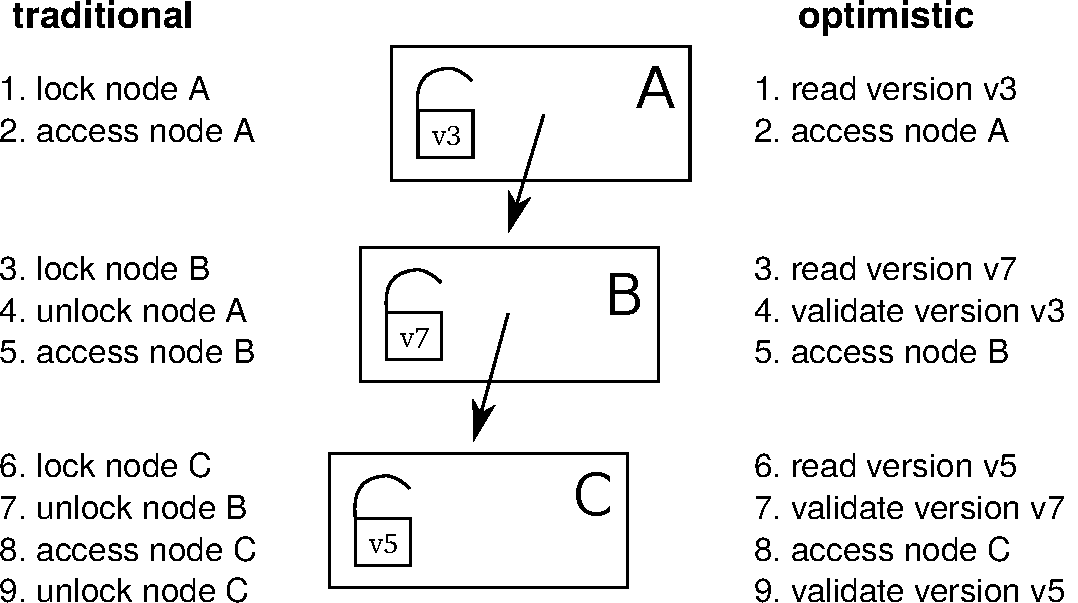
\includegraphics[width=0.65\linewidth]{olcall.pdf}
  \vspace{0.2cm}
  \caption{Comparison of a lookup operation in a 3-level tree using traditional lock coupling (left-hand side) vs.~optimistic lock coupling (right-hand side).}
  \label{fig:olc}
\end{figure}

The traditional and most common lock-based synchronization protocol for B-trees is lock coupling, which interleaves lock acquisitions while holding at most two locks at a time.
If, as we observed earlier, optimistic locks have similar semantics as traditional locks, it is natural to ask whether lock coupling can be combined with optimistic locks.
And indeed the answer is yes: One can almost mechanically translate traditional lock coupling code to optimistic lock coupling code.
This is illustrated in Figure~\ref{fig:olc}, which compares the traversal in a tree of height 3 using traditional and optimistic locks.
As the figure shows, the main difference is that locking is translated to reading the version and that unlocking becomes validation of the previously read version.
This simple change provides efficient lock-free tree traversal without the need to design a complex synchronization protocol.

It is important to emphasize the conceptual simplicity of OLC in comparison to data structures that use custom protocols like the Bw-tree~\cite{DBLP:conf/icde/LevandoskiLS13a}.
To implement lock-free access, the Bw-tree requires an indirection table, delta nodes, complex splitting and merging logic, retry logic, etc.
OLC, on the other hand, can directly be applied to B-trees mostly by adding the appropriate optimistic locking code and without modifying the node layout itself.
Therefore, OpenBw-Tree, an open source implementation of the Bw-tree, requires an order of magnitude more code than a B-tree based on OLC\footnote{Both implementations are available on GitHub: \url{https://github.com/wangziqi2016/index-microbench}}.
Given how difficult it is to develop, validate, and debug lock-free code, simplicity is obviously a major advantage.

\subsection{Correctness Aspects}

\begin{figure}
  % \centering
  %[basicstyle=\normalsize\ttfamily,showstringspaces=false,columns=fullflexible,breaklines=false,breakatwhitespace=true,numbers=none,numberstyle=\small,style=C,keepspaces=true]
\begin{lstlisting}[basicstyle=\ttfamily,language=C++,numbers=left,numberstyle=\small]
std::atomic<BTreeNode*> root;

// search for key in B+tree, returns payload in resultOut
bool lookup(Key key, Value& resultOut) {
   BTreeNode* node = root.load();
   uint64_t nodeVersion = node->readLockOrRestart();
   if (node != root.load()) // make sure the root is still the root
      restart();

   BTreeInner<Key>* parent = nullptr;
   uint64_t parentVersion = 0;

   while (node->isInner()) {
      auto inner = (BTreeInner*)node;

      // unlock parent and make current node the parent
      if (parent)
         parent->readUnlockOrRestart(parentVersion);
      parent = inner;
      parentVersion = nodeVersion;

      // search for next node
      node = inner->findChild(key);
      // validate 'inner' to ensure that 'node' pointer is valid
      inner->checkOrRestart(nodeVersion);
      // now it safe to dereference 'node' pointer (read its version)
      nodeVersion = node->readLockOrRestart();
   }

   // search in leaf and retrieve payload
   auto leaf = (BTreeLeaf*)node;
   bool success = leaf->findValue(key, resultOut);

   // unlock everything
   if (parent)
      parent->readUnlockOrRestart(parentVersion);
   node->readUnlockOrRestart(nodeVersion);

   return success;
}
\end{lstlisting}
  \vspace{0.2cm}
  \caption{B-tree lookup code using OLC. For simplicity, the restart logic is not shown.}
  \label{fig:lookup}
\end{figure}

So far, we have introduced the high-level ideas behind OLC and have stressed its similarity to traditional lock coupling.
Let us now discuss some cases where the close similarity between lock coupling and OLC breaks down.
To make this more concrete, we show the B-tree lookup code in Figure~\ref{fig:lookup}.
In the code, \texttt{readLockOrRestart} reads the lock version and \texttt{readUnlockOrRestart} validates that the read was correct.

One issue with OLC is that any pointer speculatively read from a node may point to invalid memory (if that node is modified concurrently).
Dereferencing such a pointer (e.g., to read its optimistic lock), may cause a segmentation fault or undefined behavior.
In the code shown in Figure~\ref{fig:lookup}, this problem is prevented by the extra check in line 25, which ensures that the read from the node containing the pointer was correct.
Without this additional validation, the code would in line 27 dereference the pointer speculatively read in line 23.
Note that the implementation of \texttt{checkOrRestart} is actually identical to \texttt{readUnlockOrRestart}.
We chose to give it a different name to highlight the fact that this extra check would not be necessary with read/write locks.

Another potential issue with optimistic locks is code that does not terminate.
Code that speculatively accesses a node, like an intra-node binary search, should be written in a way such that it always terminates---even in the presence of concurrent writes.
Otherwise, the validation code that detects the concurrent write will never run.
The binary search of a B-tree, for example, needs to be written in such a way that each comparison makes progress.
For some data structures that do not require loops in the traversal code (like ART) termination is trivially true.

\subsection{Implementation Details}

% implementation, efficiency
To implement an optimistic lock, one can combine the lock and the version counter into a single 64-bit\footnote{Even after subtracting one bit for the lock status, a back-of-the-envelope calculation can show that 63 bits are large enough to never overflow in practice.} word~\cite{artsync}.
A typical read operation will therefore merely consist of reading this version counter atomically.
In C++11 this can be implemented using the \texttt{std::atomic} type.

On x86, atomic reads are cheap because of x86's strong memory order guarantees.
No memory fences are required for sequentially-consistent loads, which are translated (by both GCC and clang) into standard \texttt{MOV} instructions.
Hence, the only effect of \texttt{std::atomic} for loads is preventing instruction re-ordering.
This makes version access and validation cheap.
Acquiring and releasing an optimistic lock in exclusive mode has comparable cost to a traditional lock:
A fairly expensive sequentially-consistent store is needed for acquiring a lock, while a standard \texttt{MOV} suffices for releasing it.
A simple sinlock-based implementation of optimistic locks can be found in the appendix of an earlier paper~\cite{artsync}.

OLC code must be able to handle restarts since validation or lock upgrade can fail due to concurrent writers.
Restarts can easily be implemented by wrapping the data structure operation in a loop (for simplicity not shown in Figure~\ref{fig:lookup}).
Such a loop also enables limiting the number of optimistic retry operations and falling back to pessimistic locking in cases of very heavy contention.
The ability to fall back to traditional locking is a major advantage of OLC in terms of robustness over lock-free approaches, which do not have this option.

In addition to the optimistic shared mode and the exclusive mode, optimistic locks also support a ``shared pessimistic'' mode, which physically acquires the lock in shared mode (allowing multiple concurrent readers but no writers).
This mode is useful for table (or range) scans that touch many tuples on a leaf page (which would otherwise easily abort).
Finally, let us mention that large range scans and table scans, should be broken up into several per-node traversals as is done in the LeanStore~\cite{leanstore} system.

Like all lock-free data structures, but unlike traditional locking and Hardware Transactional Memory~\cite{DBLP:conf/hpca/KarnagelDRLLSL14,DBLP:journals/pvldb/MakreshanskiLS15,htmtkde}, OLC requires care when deleting (and reusing) nodes.
The reason is that a deleting thread can never be sure that a node can be reclaimed because other threads might still be optimistically reading from that node.
Therefore, standard solutions like epoch-based reclamation~\cite{DBLP:conf/sosp/TuZKLM13}, hazard pointers~\cite{DBLP:journals/tpds/Michael04}, or optimized hazard pointers~\cite{DBLP:conf/spaa/BalmauGHZ16} need to be used.
These memory reclamation techniques are, however, largely orthogonal to the synchronization protocol itself.

%-lock-free is not a strong guarantee

\newpage
\section{Evaluation}\label{sec:evaluation}

Let us now experimentally evaluate the overhead and scalability of OLC.
For the experiments, we use an in-memory B+tree implemented in C++11 using templates, which is configured to use nodes of 4096 bytes, random 8 byte keys, and 8 byte payloads.
Based on this B-tree, we compare the following synchronization approaches:
\begin{itemize}
\item an OLC implementation\footnote{An almost identical OLC implementation is available on github: \url{https://github.com/wangziqi2016/index-microbench/tree/master/BTreeOLC}}
\item a variant based on traditional lock coupling and read/write locks
\item the unsynchronized B-tree, which obviously is only correct for read-only workloads but allows measuring the overhead of synchronization
\end{itemize}
Note that earlier work has compared the OLC implementation with a Bw-tree implementation~\cite{buzzword} and other state-of-the-art in-memory index structures.

We use a Haswell EP system with an Intel Xeon E5-2687W v3 CPU, which has 10 cores (20 ``Hyper-Threads'') and 25~MB of L3 cache.
The system is running Ubuntu 18.10 and we use GCC 8.2.0 to compile our code.
The CPU counters are obtained using the Linux perf API\footnote{We use the following convenience wrapper: \url{https://github.com/viktorleis/perfevent}}.

\begin{table}
  \caption{Performance and CPU counters for lookup and insert operations in a B-tree with 100M keys. We perform 100M operations and normalize the CPU counters by that number.}
  \label{tab:overhead}
  \centering
  \begin{tabular}{lrrrrrrr}\toprule
                    &         &        &        & instruc-  & L1     & L3     & branch \\
                    & threads & M op/s & cycles & tions & misses & misses & misses \\\midrule
lookup (no sync.)   & 1       & 1.72   & 2028   & 283     & 39.1   & 14.9   & 16.1   \\
lookup (OLC)        & 1       & 1.65   & 2107   & 370     & 43.9   & 15.1   & 16.7   \\
lookup (lock coup.) & 1       & 1.72   & 2078   & 365     & 42.3   & 16.9   & 15.7   \\\midrule
insert (no sync.)   & 1       & 1.51   & 2286   & 530     & 59.8   & 31.1   & 17.3   \\
insert (OLC)        & 1       & 1.50   & 2303   & 629     & 61.2   & 31.1   & 16.5   \\
insert (lock coup.) & 1       & 1.41   & 2473   & 644     & 61.0   & 31.0   & 17.2   \\\midrule
lookup (no sync.)   & 10      & 15.48  & 2058   & 283     & 38.6   & 15.5   & 16.0   \\
lookup (OLC)        & 10      & 14.60  & 2187   & 370     & 43.8   & 15.8   & 16.8   \\
lookup (lock coup.) & 10      & 5.71   & 5591   & 379     & 54.2   & 17.0   & 14.8   \\\midrule
insert (no sync.)   & 10      & -      & -      & -       & -      & -      & -      \\
insert (OLC)        & 10      & 10.46  & 2940   & 656     & 62.0   & 32.5   & 16.8   \\
insert (lock coup.) & 10      & 7.55   & 4161   & 667     & 75.0   & 28.6   & 16.2   \\
    \bottomrule
\end{tabular}
\end{table}

Table~\ref{tab:overhead} compares the performance and CPU counters for lookup and insert operations in a B-tree with 100M keys.
With {\em single-threaded} execution, we observe that all three approaches have very similar performance.
Adding traditional or optimistic locks to unsynchronized B-tree code results in up to 30\% of additional instructions without affecting single-threaded performance much.

\begin{figure}
  \centering
  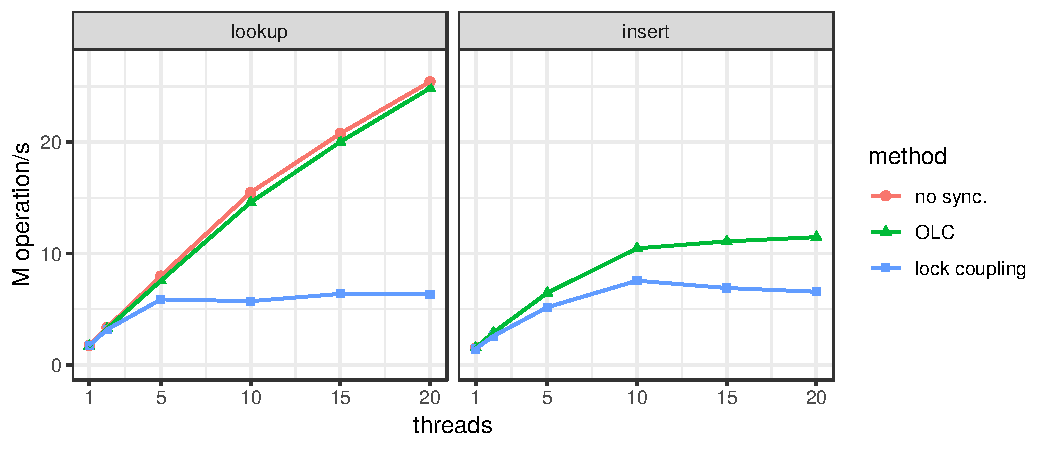
\includegraphics[width=\linewidth]{scale.pdf}
  \vspace{0.2cm}
  \caption{Scalability on 10-core system for B-tree operations (100M values).}
  \label{fig:scale}
\end{figure}

As Figure~\ref{fig:scale} shows, the results change dramatically once we use multiple threads.
For lookup, the scalability of OLC is near-linear up to 20 threads, even though the system has only 10 ``real cores''.
The OLC scalability for insert is also respectable (though not quite as linear because multi-threaded insertion approaches the memory bandwidth of our processor).
The figure also shows that the results of traditional lock coupling with read/write locks are significantly worse than OLC.
With 20 threads, lookup with OLC is 3.9$\times$ faster than traditional lock coupling.

\section{Summary}\label{sec:conc}

Optimistic Lock Coupling (OLC) is an effective synchronization method that combines the simplicity of traditional lock coupling with the superior scalability of lock-free approaches.
OLC is widely applicable and has already been successfully used to synchronize several data structures, including B-trees, binary search trees, and different trie variants.
These features make it highly attractive for modern database systems as well as performance-critical systems software in general.

\begin{thebibliography}{10}

\bibitem{DBLP:conf/spaa/BalmauGHZ16}
O.~Balmau, R.~Guerraoui, M.~Herlihy, and I.~Zablotchi.
\newblock Fast and robust memory reclamation for concurrent data structures.
\newblock In {\em SPAA}, 2016.

\bibitem{DBLP:journals/acta/BayerS77}
R.~Bayer and M.~Schkolnick.
\newblock Concurrency of operations on {B}-trees.
\newblock {\em Acta Informatica}, 9, 1977.

\bibitem{hot}
R.~Binna, E.~Zangerle, M.~Pichl, G.~Specht, and V.~Leis.
\newblock {HOT}: A height optimized trie index for main-memory database
  systems.
\newblock In {\em SIGMOD}, 2018.

\bibitem{DBLP:conf/ppopp/BronsonCCO10}
N.~G. Bronson, J.~Casper, H.~Chafi, and K.~Olukotun.
\newblock A practical concurrent binary search tree.
\newblock In {\em PPOPP}, 2010.

\bibitem{DBLP:conf/vldb/ChaHKK01}
S.~K. Cha, S.~Hwang, K.~Kim, and K.~Kwon.
\newblock Cache-conscious concurrency control of main-memory indexes on
  shared-memory multiprocessor systems.
\newblock In {\em VLDB}, 2001.

\bibitem{intel}
I.~Cutress.
\newblock {Intel} goes for 48-cores: {Cascade-AP} with multi-chip package
  coming soon.
\newblock
  \url{https://www.anandtech.com/show/13535/intel-goes-for-48cores-cascade-ap},
  2018 (accessed January, 2019).

\bibitem{DBLP:conf/cidr/FaleiroA17}
J.~M. Faleiro and D.~J. Abadi.
\newblock Latch-free synchronization in database systems: Silver bullet or
  fool's gold?
\newblock In {\em CIDR}, 2017.

\bibitem{DBLP:journals/ftdb/Graefe11}
G.~Graefe.
\newblock Modern {B}-tree techniques.
\newblock {\em Foundations and Trends in Databases}, 3(4), 2011.

\bibitem{DBLP:conf/hpca/KarnagelDRLLSL14}
T.~Karnagel, R.~Dementiev, R.~Rajwar, K.~Lai, T.~Legler, B.~Schlegel, and
  W.~Lehner.
\newblock Improving in-memory database index performance with
  {Intel}\({}^{\mbox{{\textregistered}}}\) transactional synchronization
  extensions.
\newblock In {\em HPCA}, 2014.

\bibitem{DBLP:journals/tods/LehmanY81}
P.~L. Lehman and S.~B. Yao.
\newblock Efficient locking for concurrent operations on {B}-trees.
\newblock {\em {ACM} Trans. Database Syst.}, 6(4), 1981.

\bibitem{leanstore}
V.~Leis, M.~Haubenschild, A.~Kemper, and T.~Neumann.
\newblock Leanstore: In-memory data management beyond main memory.
\newblock In {\em ICDE}, 2018.

\bibitem{art}
V.~Leis, A.~Kemper, and T.~Neumann.
\newblock The adaptive radix tree: {ARTful} indexing for main-memory databases.
\newblock In {\em ICDE}, 2013.

\bibitem{htmtkde}
V.~Leis, A.~Kemper, and T.~Neumann.
\newblock Scaling {HTM}-supported database transactions to many cores.
\newblock {\em {IEEE} Trans. Knowl. Data Eng.}, 28(2), 2016.

\bibitem{artsync}
V.~Leis, F.~Scheibner, A.~Kemper, and T.~Neumann.
\newblock The {ART} of practical synchronization.
\newblock In {\em DaMoN}, 2016.

\bibitem{DBLP:conf/icde/LevandoskiLS13a}
J.~J. Levandoski, D.~B. Lomet, and S.~Sengupta.
\newblock The {Bw}-tree: A {B}-tree for new hardware platforms.
\newblock In {\em ICDE}, 2013.

\bibitem{DBLP:journals/pvldb/MakreshanskiLS15}
D.~Makreshanski, J.~J. Levandoski, and R.~Stutsman.
\newblock To lock, swap, or elide: On the interplay of hardware transactional
  memory and lock-free indexing.
\newblock {\em {PVLDB}}, 8(11), 2015.

\bibitem{DBLP:dblp_conf/eurosys/MaoKM12}
Y.~Mao, E.~Kohler, and R.~T. Morris.
\newblock Cache craftiness for fast multicore key-value storage.
\newblock In {\em EuroSys}, 2012.

\bibitem{DBLP:journals/tpds/Michael04}
M.~M. Michael.
\newblock Hazard pointers: Safe memory reclamation for lock-free objects.
\newblock {\em {IEEE} Trans. Parallel Distrib. Syst.}, 15(6), 2004.

\bibitem{DBLP:journals/jacm/ShalevS06}
O.~Shalev and N.~Shavit.
\newblock Split-ordered lists: Lock-free extensible hash tables.
\newblock {\em J. {ACM}}, 53(3), 2006.

\bibitem{amd}
A.~Shilov.
\newblock {AMD} previews {EPYC} ‘{Rome}’ processor: Up to 64 {Zen} 2 cores.
\newblock
  \url{https://www.anandtech.com/show/13561/amd-previews-epyc-rome-processor-up-to-64-zen-2-cores},
  2018 (accessed January, 2019).

\bibitem{DBLP:conf/sosp/TuZKLM13}
S.~Tu, W.~Zheng, E.~Kohler, B.~Liskov, and S.~Madden.
\newblock Speedy transactions in multicore in-memory databases.
\newblock In {\em SOSP}, 2013.

\bibitem{buzzword}
Z.~Wang, A.~Pavlo, H.~Lim, V.~Leis, H.~Zhang, M.~Kaminsky, and D.~Andersen.
\newblock Building a {Bw}-tree takes more than just buzz words.
\newblock In {\em SIGMOD}, 2018.

\end{thebibliography}


%\bibliographystyle{abbrv}
%\bibliography{main}

\end{document}

\end{article}

\begin{article}
{Validating Data and Models in Continuous ML Pipelines}
{Mike Dreves, Gene Huang, Zhuo Peng, Neoklis Polyzotis, Evan Rosen and Paul Suganthan G. C.}
\pdfminorversion=5
\documentclass[11pt]{article}
\usepackage{deauthor,times,graphicx,caption,microtype}
\usepackage{hyperref}
\usepackage{listings}
\usepackage{booktabs}

\begin{document}

\title{Optimistic Lock Coupling: A Scalable and Efficient General-Purpose Synchronization Method}

\author{Viktor Leis, Michael Haubenschild\raisebox{0.9ex}{$\ast$}, Thomas Neumann\\ Technische Universit{\"a}t M{\"u}nchen \hspace{0.7cm} Tableau Software\raisebox{0.9ex}{$\ast$} \\ {\{leis,neumann\}{@}in.tum.de} \hspace{0.7cm} {mhaubenschild{@}tableau.com\raisebox{0.9ex}{$\ast$}}}

\maketitle

\begin{abstract}
As the number of cores on commodity processors continues to increase, scalability becomes more and more crucial for overall performance.
Scalable and efficient concurrent data structures are particularly important, as these are often the building blocks of parallel algorithms.
Unfortunately, traditional synchronization techniques based on fine-grained locking have been shown to be unscalable on modern multi-core CPUs.
Lock-free data structures, on the other hand, are extremely difficult to design and often incur significant overhead.

In this work, we make the case for Optimistic Lock Coupling as a practical alternative to both traditional locking and the lock-free approach.
We show that Optimistic Lock Coupling is highly scalable and almost as simple to implement as traditional lock coupling.
Another important advantage is that it is easily applicable to most tree-like data structures.
We therefore argue that Optimistic Lock Coupling, rather than a complex and error-prone custom synchronization protocol, should be the default choice for performance-critical data structures.
\end{abstract}

\section{Introduction}

% more and more cores
Today, Intel's commodity server processors have up to 28 cores and its upcoming microarchitecture will have up to 48 cores per socket~\cite{intel}.
Similarly, AMD currently stands at 32 cores and this number is expected to double in the next generation~\cite{amd}.
Since both platforms support simultaneous multithreading (also known as hyperthreading), affordable commodity servers (with up to two sockets) will soon routinely have between 100 and 200 hardware threads.

% data structure scalability is important
With such a high degree of hardware parallelism, efficient data processing crucially depends on how well concurrent data structures scale.
Internally, database systems use a plethora of data structures like table heaps, internal work queues, and, most importantly, index structures.
Any of these can easily become a scalability (and therefore overall performance) bottleneck on many-core CPUs.

% traditional synchronization: fine-grained locks, slow, cache invalidation
Traditionally, database systems synchronize internal data structures using fine-grained reader/writer locks\footnote{In this work, we focus on data structure synchronization rather than high-level transaction semantics and therefore use the term {\em lock} for what would typically be called {\em latch} in the database literature. We thus follow common computer science (rather than database) terminology.}.
Unfortunately, while fine-grained locking makes lock contention unlikely, it still results in bad scalability because lock acquisition and release require writing to shared memory.
Due to the way cache coherency is implemented on modern multi-core CPUs, these writes cause additional cache misses\footnote{The cache coherency protocol ensures that all copies of a cache line on other cores are invalidated before the write can proceed.} and the cache line containing the lock's internal data becomes a point of physical contention.
As a result, any frequently-accessed lock (e.g., the lock of the root node of a B-tree) severely limits scalability.

% lock-free bw-tree: no more latches, but indirections, extremely complex
Lock-free data structures like the Bw-tree~\cite{DBLP:conf/icde/LevandoskiLS13a} (a lock-free B-tree variant) or the Split-Ordered List~\cite{DBLP:journals/jacm/ShalevS06} (a lock-free hash table) do not acquire any locks and therefore generally scale much better than locking-based approaches (in particular for read-mostly workloads).
However, lock-free synchronization has other downsides:
First, it is very difficult and results in extremely complex and error-prone code (when compared to locking).
Second, because the functionality of atomic primitives provided by the hardware (e.g., atomically compare-and-swap 8 bytes) is limited, complex operations require additional indirections within the data structure.
For example, the Bw-tree requires an indirection table and the Split-Ordered List requires ``dummy nodes'', resulting in overhead due to additional cache misses.

% OLC for the win
In this paper we make the case for {\em Optimistic Lock Coupling (OLC)}, a synchronization method that combines some of the best properties of lock-based and lock-free synchronization.
OLC utilizes a special lock type that can be used in two modes:
The first mode is similar to a traditional mutex and excludes other threads by physically acquiring the underlying lock.
In the second mode, reads can proceed optimistically by validating a version counter that is embedded in the lock (similar to optimistic concurrency control).
The first mode is typically used by writers and the second mode by readers.
Besides this special lock type, OLC is based on the observation that optimistic lock validations can be interleaved/coupled---similar to the pair-wise interleaved lock acquisition of traditional lock coupling.
Hence, the name Optimistic Lock Coupling.

OLC has a number of desirable features:
\begin{itemize}
\item By reducing the number of writes to shared memory locations and thereby avoiding cache invalidations, it {\bf scales well} for most workloads.
\item In comparison to unsynchronized code, it requires few additional CPU instructions making it {\bf efficient}.
\item OLC is {\bf widely applicable} to different data structures. It has already been successfully used for synchronizing binary search trees~\cite{DBLP:conf/ppopp/BronsonCCO10}, tries~\cite{artsync}, trie/B-tree hybrids~\cite{DBLP:dblp_conf/eurosys/MaoKM12}, and B-trees~\cite{buzzword}.
\item In comparison to the lock-free paradigm, it is also {\bf easy to use} and requires few modifications to existing, single-threaded data structures.
\end{itemize}
Despite these positive features and its simplicity, OLC is not yet widely known.
The goal of this paper is therefore to popularize this simple idea and to make a case for it.
We argue that OLC deserves to be widely known.
It is a good default synchronization paradigm---more complex, data structure-specific protocols are seldom beneficial.

The rest of the paper is organized as follows.
Section~\ref{sec:related} discusses related work, tracing the history of OLC and its underlying ideas in the literature.
The core of the paper is Section~\ref{sec:olc}, which describes the ideas behind OLC and how it can be used to synchronize complex data structures.
In Section~\ref{sec:evaluation} we experimentally show that OLC has low overhead and scales well when used to synchronize an in-memory B-tree.
We summarize the paper in Section~\ref{sec:conc}.

\newpage
\section{Related Work}\label{sec:related}

Lock coupling has been proposed as a method for allowing concurrent operations on B-trees in 1977~\cite{DBLP:journals/acta/BayerS77}.
This traditional and still widely-used method, described in detail in Graefe's B-tree survey~\cite{DBLP:journals/ftdb/Graefe11}, is also called ``latch coupling'', ``hand-over-hand locking'', and ``crabbing''.
Because at most two locks are held at-a-time during tree traversal, this technique seemingly allows for a high degree of parallelism---in particular if read/write locks are used to enable inner nodes to be locked in shared mode.
However, as we show in Section~\ref{sec:evaluation}, on modern hardware lock acquisition (even in shared mode) results in suboptimal scalability.

An early alternative from 1981 is a B-tree variant called B-link tree~\cite{DBLP:journals/tods/LehmanY81}, which only holds a single lock at a time.
It is based on the observation that between the release of the parent lock and the acquisition of the child lock, the only ``dangerous'' thing that could have happened is the split of a child node (assuming one does not implement merge operations).
Thus, when a split happens, the key being searched might end up on a neighboring node to the right of the current child node.
A B-link tree traversal therefore detects this condition and, if needed, transparently proceeds to the neighboring node.
Releasing the parent lock early is highly beneficial when the child node needs to be fetched from disk.
For in-memory workloads, however, the B-link tree has the same scalability issues as lock coupling (it acquires just as many locks).

The next major advance, Optimistic Latch-Free Index Traversal (OLFIT)~\cite{DBLP:conf/vldb/ChaHKK01}, was proposed in 2001.
OLFIT introduced the idea of a combined lock/update counter, which we call {\em optimistic lock}. % , for lack of a better name,
Based on these per-node optimistic locks and the synchronization protocol of the B-link tree, OLFIT finally achieves good scalability on parallel processors.
The OLFIT protocol is fairly complex, as it requires both the non-trivial B-link protocol and optimistic locks.
Furthermore, like the B-link tree protocol, it does not support merging nodes, and is specific to B-trees (cannot easily be applied to other data structures).

In the following two decades, the growth of main-memory capacity led to much research into other data structures besides the venerable B-tree.
Particularly relevant for our discussion is Bronson et al.'s~\cite{DBLP:conf/ppopp/BronsonCCO10} concurrent binary search tree, which is based on optimistic version validation and has a sophisticated, data structure-specific synchronization protocol.
To the best of our knowledge, this 2010 paper is the first that, as part of its protocol, interleaves version validation across nodes---rather than validating each node separately like OLFIT.
In that paper, this idea is called ``hand-over-hand, optimistic validation'', while we prefer the term Optimistic Lock Coupling to highlight the close resemblance to traditional lock coupling.
Similarly, Mao et al.'s~\cite{DBLP:dblp_conf/eurosys/MaoKM12} Masstree (a concurrent hybrid trie/B-tree) is also based on the same ideas, but again uses them as part of a more complex protocol.

The Adaptive Radix Tree (ART)~\cite{art} is another recent in-memory data structure, which we proposed in 2013.
In contrast to the two data structures just mentioned, it was originally designed with single-threaded performance in mind without supporting concurrency.
To add support for concurrency, we initially started designing a custom protocol called Read-Optimized Write Exclusion (ROWEX)~\cite{artsync}, which turned out to be non-trivial and requires modifications of the underlying data structure\footnote{Note that ROWEX is already easier to apply to existing data structures than the lock-free approach. The difficulty depends on the data structure. Applying ROWEX is hard for B-trees with sorted keys and fairly easy for copy-on-write data structures like the Height Optimized Trie~\cite{hot}---with ART being somewhere in the middle.}.
However, fairly late in the project, we also realized, that OLC {\em alone} (rather than as part of a more complex protocol) is sufficient to synchronize ART.
No other changes to the data structure were necessary.
Both approaches were published and experimentally evaluated in a followup paper~\cite{artsync}, which shows that, despite its simplicity, OLC is efficient, scalable, and generally outperforms ROWEX.

Similar results were recently published regarding B-trees~\cite{buzzword}.
In this experimental study a simple OLC-based synchronization outperformed the Bw-tree~\cite{DBLP:conf/icde/LevandoskiLS13a}, a complex lock-free synchronization approach.
Another recent paper shows that for write-intensive workloads, locking often performs better than lock-free synchronization~\cite{DBLP:conf/cidr/FaleiroA17}.
These experiences indicate that OLC is a general-purpose synchronization paradigm and motivate the current paper.

%foster b-tree\cite{DBLP:journals/tods/GraefeKK12}
%Shasha theory~\cite{DBLP:journals/tods/ShashaG88}

\section{Optimistic Lock Coupling}\label{sec:olc}

% locks suck
The standard technique for inter-thread synchronization is mutual exclusion using fine-grained locks.
In a B-tree, for example, every node usually has its own associated lock, which is acquired before accessing that node.
The problem of locking on modern multi- and many-core processors is that lock acquisition and release require writing to the shared memory location that implements the lock.
This write causes exclusive ownership of the underlying cache line and invalidates copies of it on all other processor cores.
For hierarchical, tree-like data structures, the lock of the root node becomes a point of physical contention---even in read-only workloads and even when read/write locks are used.
Depending on the specific data structure, number of cores, cache coherency protocol implementation, cache topology, whether Non-Uniform Memory Access (NUMA) is used, locking can even result in multi-threaded performance that is worse than single-threaded execution.

% in b-trees this happens very much
The inherent pessimism of locking is particularly unfortunate for B-trees:
Despite the fact that logical modifications of the root node are very infrequent, every B-tree operation must lock the root node during tree traversal\footnote{To a lesser extent this obviously applies to all inner nodes, not just the root.}.
Even the vast majority of update operations (with the exception of splits and merges), only modify a single leaf node.
These observations indicate that a more optimistic approach, which does not require locking inner nodes, would be very beneficial for B-trees.

\subsection{Optimistic Locks}

% optimism to the rescue
As the name indicates, optimistic locks try to solve the scalability issues of traditional locks using an optimistic approach.
Instead of always physically acquiring locks, even for nodes that are unlikely to be modified simultaneously, after-the-fact validation is used to detect conflicts.
This is done by augmenting each lock with a version/update counter that is incremented on every modification.
Using this version counter, readers can optimistically proceed before validating that the version did not change to ensure that the read was safe.
If validation fails, the operation is restarted.

% details on opt locks
Using optimistic locks, a read-only node access (i.e., the majority of all operations in a B-tree) does not acquire the lock and does not increment the version counter.
Instead, it performs the following steps:
\begin{enumerate}
\item read lock version (restart if lock is not free)
\item access node
\item read the version again and validate that it has not changed in the meantime
\end{enumerate}
If the last step (the validation) fails, the operation has to be restarted.
Write operations, on the other hand, are more similar to traditional locking:
\begin{enumerate}
\item acquire lock (wait if necessary)
\item access/write to node
\item increment version and unlock node
\end{enumerate}
Writes can therefore protect a node from other writes.

% similar to locks
As we observed in an earlier paper~\cite{artsync}, because of similar semantics, optimistic locks can be hidden behind an API very similar to traditional read/write locks.
Both approaches have an exclusive lock mode, and acquiring a traditional lock in shared mode is analogous to optimistic version validation.
Furthermore, like with some implementations of traditional read/write locks, optimistic locks allow upgrading a shared lock to an exclusive lock.
Lock upgrades are, for example, used to avoid most B-tree update operations from having to lock inner nodes.
In our experience, the close resemblance of optimistic and traditional locks simplifies the reasoning about optimistic locks;
one can apply similar thinking as in traditional lock-based protocols.

\subsection{Lock Coupling with Optimistic Locks}

\begin{figure}
  \centering
  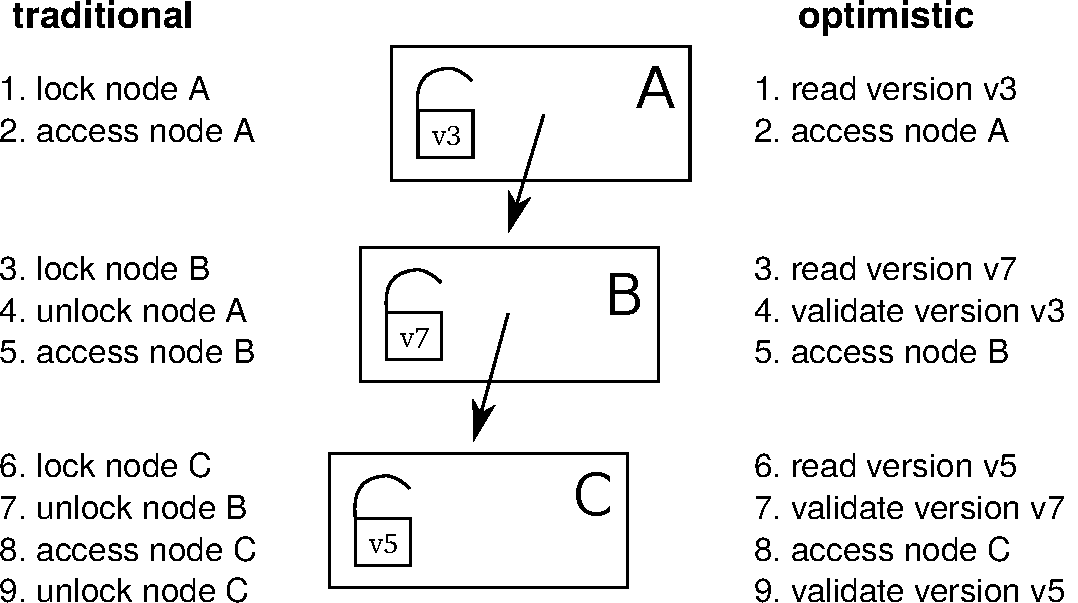
\includegraphics[width=0.65\linewidth]{olcall.pdf}
  \vspace{0.2cm}
  \caption{Comparison of a lookup operation in a 3-level tree using traditional lock coupling (left-hand side) vs.~optimistic lock coupling (right-hand side).}
  \label{fig:olc}
\end{figure}

The traditional and most common lock-based synchronization protocol for B-trees is lock coupling, which interleaves lock acquisitions while holding at most two locks at a time.
If, as we observed earlier, optimistic locks have similar semantics as traditional locks, it is natural to ask whether lock coupling can be combined with optimistic locks.
And indeed the answer is yes: One can almost mechanically translate traditional lock coupling code to optimistic lock coupling code.
This is illustrated in Figure~\ref{fig:olc}, which compares the traversal in a tree of height 3 using traditional and optimistic locks.
As the figure shows, the main difference is that locking is translated to reading the version and that unlocking becomes validation of the previously read version.
This simple change provides efficient lock-free tree traversal without the need to design a complex synchronization protocol.

It is important to emphasize the conceptual simplicity of OLC in comparison to data structures that use custom protocols like the Bw-tree~\cite{DBLP:conf/icde/LevandoskiLS13a}.
To implement lock-free access, the Bw-tree requires an indirection table, delta nodes, complex splitting and merging logic, retry logic, etc.
OLC, on the other hand, can directly be applied to B-trees mostly by adding the appropriate optimistic locking code and without modifying the node layout itself.
Therefore, OpenBw-Tree, an open source implementation of the Bw-tree, requires an order of magnitude more code than a B-tree based on OLC\footnote{Both implementations are available on GitHub: \url{https://github.com/wangziqi2016/index-microbench}}.
Given how difficult it is to develop, validate, and debug lock-free code, simplicity is obviously a major advantage.

\subsection{Correctness Aspects}

\begin{figure}
  % \centering
  %[basicstyle=\normalsize\ttfamily,showstringspaces=false,columns=fullflexible,breaklines=false,breakatwhitespace=true,numbers=none,numberstyle=\small,style=C,keepspaces=true]
\begin{lstlisting}[basicstyle=\ttfamily,language=C++,numbers=left,numberstyle=\small]
std::atomic<BTreeNode*> root;

// search for key in B+tree, returns payload in resultOut
bool lookup(Key key, Value& resultOut) {
   BTreeNode* node = root.load();
   uint64_t nodeVersion = node->readLockOrRestart();
   if (node != root.load()) // make sure the root is still the root
      restart();

   BTreeInner<Key>* parent = nullptr;
   uint64_t parentVersion = 0;

   while (node->isInner()) {
      auto inner = (BTreeInner*)node;

      // unlock parent and make current node the parent
      if (parent)
         parent->readUnlockOrRestart(parentVersion);
      parent = inner;
      parentVersion = nodeVersion;

      // search for next node
      node = inner->findChild(key);
      // validate 'inner' to ensure that 'node' pointer is valid
      inner->checkOrRestart(nodeVersion);
      // now it safe to dereference 'node' pointer (read its version)
      nodeVersion = node->readLockOrRestart();
   }

   // search in leaf and retrieve payload
   auto leaf = (BTreeLeaf*)node;
   bool success = leaf->findValue(key, resultOut);

   // unlock everything
   if (parent)
      parent->readUnlockOrRestart(parentVersion);
   node->readUnlockOrRestart(nodeVersion);

   return success;
}
\end{lstlisting}
  \vspace{0.2cm}
  \caption{B-tree lookup code using OLC. For simplicity, the restart logic is not shown.}
  \label{fig:lookup}
\end{figure}

So far, we have introduced the high-level ideas behind OLC and have stressed its similarity to traditional lock coupling.
Let us now discuss some cases where the close similarity between lock coupling and OLC breaks down.
To make this more concrete, we show the B-tree lookup code in Figure~\ref{fig:lookup}.
In the code, \texttt{readLockOrRestart} reads the lock version and \texttt{readUnlockOrRestart} validates that the read was correct.

One issue with OLC is that any pointer speculatively read from a node may point to invalid memory (if that node is modified concurrently).
Dereferencing such a pointer (e.g., to read its optimistic lock), may cause a segmentation fault or undefined behavior.
In the code shown in Figure~\ref{fig:lookup}, this problem is prevented by the extra check in line 25, which ensures that the read from the node containing the pointer was correct.
Without this additional validation, the code would in line 27 dereference the pointer speculatively read in line 23.
Note that the implementation of \texttt{checkOrRestart} is actually identical to \texttt{readUnlockOrRestart}.
We chose to give it a different name to highlight the fact that this extra check would not be necessary with read/write locks.

Another potential issue with optimistic locks is code that does not terminate.
Code that speculatively accesses a node, like an intra-node binary search, should be written in a way such that it always terminates---even in the presence of concurrent writes.
Otherwise, the validation code that detects the concurrent write will never run.
The binary search of a B-tree, for example, needs to be written in such a way that each comparison makes progress.
For some data structures that do not require loops in the traversal code (like ART) termination is trivially true.

\subsection{Implementation Details}

% implementation, efficiency
To implement an optimistic lock, one can combine the lock and the version counter into a single 64-bit\footnote{Even after subtracting one bit for the lock status, a back-of-the-envelope calculation can show that 63 bits are large enough to never overflow in practice.} word~\cite{artsync}.
A typical read operation will therefore merely consist of reading this version counter atomically.
In C++11 this can be implemented using the \texttt{std::atomic} type.

On x86, atomic reads are cheap because of x86's strong memory order guarantees.
No memory fences are required for sequentially-consistent loads, which are translated (by both GCC and clang) into standard \texttt{MOV} instructions.
Hence, the only effect of \texttt{std::atomic} for loads is preventing instruction re-ordering.
This makes version access and validation cheap.
Acquiring and releasing an optimistic lock in exclusive mode has comparable cost to a traditional lock:
A fairly expensive sequentially-consistent store is needed for acquiring a lock, while a standard \texttt{MOV} suffices for releasing it.
A simple sinlock-based implementation of optimistic locks can be found in the appendix of an earlier paper~\cite{artsync}.

OLC code must be able to handle restarts since validation or lock upgrade can fail due to concurrent writers.
Restarts can easily be implemented by wrapping the data structure operation in a loop (for simplicity not shown in Figure~\ref{fig:lookup}).
Such a loop also enables limiting the number of optimistic retry operations and falling back to pessimistic locking in cases of very heavy contention.
The ability to fall back to traditional locking is a major advantage of OLC in terms of robustness over lock-free approaches, which do not have this option.

In addition to the optimistic shared mode and the exclusive mode, optimistic locks also support a ``shared pessimistic'' mode, which physically acquires the lock in shared mode (allowing multiple concurrent readers but no writers).
This mode is useful for table (or range) scans that touch many tuples on a leaf page (which would otherwise easily abort).
Finally, let us mention that large range scans and table scans, should be broken up into several per-node traversals as is done in the LeanStore~\cite{leanstore} system.

Like all lock-free data structures, but unlike traditional locking and Hardware Transactional Memory~\cite{DBLP:conf/hpca/KarnagelDRLLSL14,DBLP:journals/pvldb/MakreshanskiLS15,htmtkde}, OLC requires care when deleting (and reusing) nodes.
The reason is that a deleting thread can never be sure that a node can be reclaimed because other threads might still be optimistically reading from that node.
Therefore, standard solutions like epoch-based reclamation~\cite{DBLP:conf/sosp/TuZKLM13}, hazard pointers~\cite{DBLP:journals/tpds/Michael04}, or optimized hazard pointers~\cite{DBLP:conf/spaa/BalmauGHZ16} need to be used.
These memory reclamation techniques are, however, largely orthogonal to the synchronization protocol itself.

%-lock-free is not a strong guarantee

\newpage
\section{Evaluation}\label{sec:evaluation}

Let us now experimentally evaluate the overhead and scalability of OLC.
For the experiments, we use an in-memory B+tree implemented in C++11 using templates, which is configured to use nodes of 4096 bytes, random 8 byte keys, and 8 byte payloads.
Based on this B-tree, we compare the following synchronization approaches:
\begin{itemize}
\item an OLC implementation\footnote{An almost identical OLC implementation is available on github: \url{https://github.com/wangziqi2016/index-microbench/tree/master/BTreeOLC}}
\item a variant based on traditional lock coupling and read/write locks
\item the unsynchronized B-tree, which obviously is only correct for read-only workloads but allows measuring the overhead of synchronization
\end{itemize}
Note that earlier work has compared the OLC implementation with a Bw-tree implementation~\cite{buzzword} and other state-of-the-art in-memory index structures.

We use a Haswell EP system with an Intel Xeon E5-2687W v3 CPU, which has 10 cores (20 ``Hyper-Threads'') and 25~MB of L3 cache.
The system is running Ubuntu 18.10 and we use GCC 8.2.0 to compile our code.
The CPU counters are obtained using the Linux perf API\footnote{We use the following convenience wrapper: \url{https://github.com/viktorleis/perfevent}}.

\begin{table}
  \caption{Performance and CPU counters for lookup and insert operations in a B-tree with 100M keys. We perform 100M operations and normalize the CPU counters by that number.}
  \label{tab:overhead}
  \centering
  \begin{tabular}{lrrrrrrr}\toprule
                    &         &        &        & instruc-  & L1     & L3     & branch \\
                    & threads & M op/s & cycles & tions & misses & misses & misses \\\midrule
lookup (no sync.)   & 1       & 1.72   & 2028   & 283     & 39.1   & 14.9   & 16.1   \\
lookup (OLC)        & 1       & 1.65   & 2107   & 370     & 43.9   & 15.1   & 16.7   \\
lookup (lock coup.) & 1       & 1.72   & 2078   & 365     & 42.3   & 16.9   & 15.7   \\\midrule
insert (no sync.)   & 1       & 1.51   & 2286   & 530     & 59.8   & 31.1   & 17.3   \\
insert (OLC)        & 1       & 1.50   & 2303   & 629     & 61.2   & 31.1   & 16.5   \\
insert (lock coup.) & 1       & 1.41   & 2473   & 644     & 61.0   & 31.0   & 17.2   \\\midrule
lookup (no sync.)   & 10      & 15.48  & 2058   & 283     & 38.6   & 15.5   & 16.0   \\
lookup (OLC)        & 10      & 14.60  & 2187   & 370     & 43.8   & 15.8   & 16.8   \\
lookup (lock coup.) & 10      & 5.71   & 5591   & 379     & 54.2   & 17.0   & 14.8   \\\midrule
insert (no sync.)   & 10      & -      & -      & -       & -      & -      & -      \\
insert (OLC)        & 10      & 10.46  & 2940   & 656     & 62.0   & 32.5   & 16.8   \\
insert (lock coup.) & 10      & 7.55   & 4161   & 667     & 75.0   & 28.6   & 16.2   \\
    \bottomrule
\end{tabular}
\end{table}

Table~\ref{tab:overhead} compares the performance and CPU counters for lookup and insert operations in a B-tree with 100M keys.
With {\em single-threaded} execution, we observe that all three approaches have very similar performance.
Adding traditional or optimistic locks to unsynchronized B-tree code results in up to 30\% of additional instructions without affecting single-threaded performance much.

\begin{figure}
  \centering
  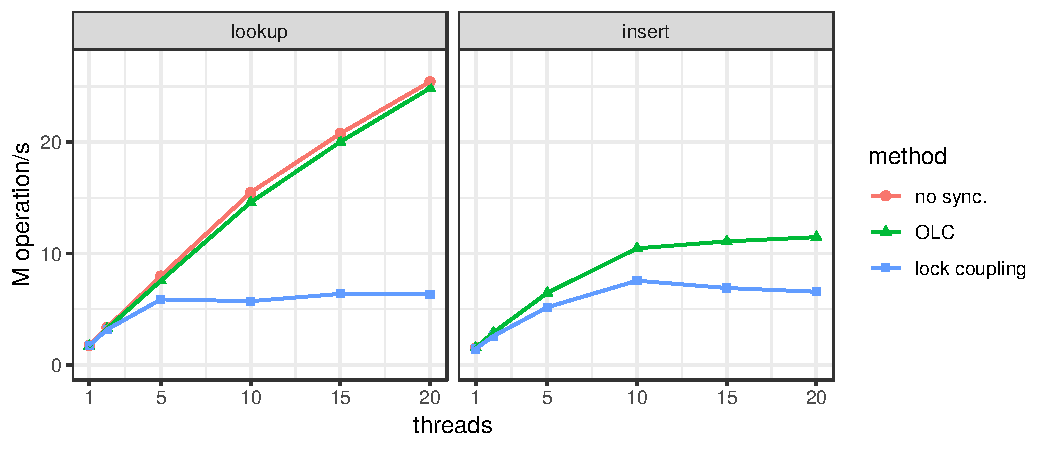
\includegraphics[width=\linewidth]{scale.pdf}
  \vspace{0.2cm}
  \caption{Scalability on 10-core system for B-tree operations (100M values).}
  \label{fig:scale}
\end{figure}

As Figure~\ref{fig:scale} shows, the results change dramatically once we use multiple threads.
For lookup, the scalability of OLC is near-linear up to 20 threads, even though the system has only 10 ``real cores''.
The OLC scalability for insert is also respectable (though not quite as linear because multi-threaded insertion approaches the memory bandwidth of our processor).
The figure also shows that the results of traditional lock coupling with read/write locks are significantly worse than OLC.
With 20 threads, lookup with OLC is 3.9$\times$ faster than traditional lock coupling.

\section{Summary}\label{sec:conc}

Optimistic Lock Coupling (OLC) is an effective synchronization method that combines the simplicity of traditional lock coupling with the superior scalability of lock-free approaches.
OLC is widely applicable and has already been successfully used to synchronize several data structures, including B-trees, binary search trees, and different trie variants.
These features make it highly attractive for modern database systems as well as performance-critical systems software in general.

\begin{thebibliography}{10}

\bibitem{DBLP:conf/spaa/BalmauGHZ16}
O.~Balmau, R.~Guerraoui, M.~Herlihy, and I.~Zablotchi.
\newblock Fast and robust memory reclamation for concurrent data structures.
\newblock In {\em SPAA}, 2016.

\bibitem{DBLP:journals/acta/BayerS77}
R.~Bayer and M.~Schkolnick.
\newblock Concurrency of operations on {B}-trees.
\newblock {\em Acta Informatica}, 9, 1977.

\bibitem{hot}
R.~Binna, E.~Zangerle, M.~Pichl, G.~Specht, and V.~Leis.
\newblock {HOT}: A height optimized trie index for main-memory database
  systems.
\newblock In {\em SIGMOD}, 2018.

\bibitem{DBLP:conf/ppopp/BronsonCCO10}
N.~G. Bronson, J.~Casper, H.~Chafi, and K.~Olukotun.
\newblock A practical concurrent binary search tree.
\newblock In {\em PPOPP}, 2010.

\bibitem{DBLP:conf/vldb/ChaHKK01}
S.~K. Cha, S.~Hwang, K.~Kim, and K.~Kwon.
\newblock Cache-conscious concurrency control of main-memory indexes on
  shared-memory multiprocessor systems.
\newblock In {\em VLDB}, 2001.

\bibitem{intel}
I.~Cutress.
\newblock {Intel} goes for 48-cores: {Cascade-AP} with multi-chip package
  coming soon.
\newblock
  \url{https://www.anandtech.com/show/13535/intel-goes-for-48cores-cascade-ap},
  2018 (accessed January, 2019).

\bibitem{DBLP:conf/cidr/FaleiroA17}
J.~M. Faleiro and D.~J. Abadi.
\newblock Latch-free synchronization in database systems: Silver bullet or
  fool's gold?
\newblock In {\em CIDR}, 2017.

\bibitem{DBLP:journals/ftdb/Graefe11}
G.~Graefe.
\newblock Modern {B}-tree techniques.
\newblock {\em Foundations and Trends in Databases}, 3(4), 2011.

\bibitem{DBLP:conf/hpca/KarnagelDRLLSL14}
T.~Karnagel, R.~Dementiev, R.~Rajwar, K.~Lai, T.~Legler, B.~Schlegel, and
  W.~Lehner.
\newblock Improving in-memory database index performance with
  {Intel}\({}^{\mbox{{\textregistered}}}\) transactional synchronization
  extensions.
\newblock In {\em HPCA}, 2014.

\bibitem{DBLP:journals/tods/LehmanY81}
P.~L. Lehman and S.~B. Yao.
\newblock Efficient locking for concurrent operations on {B}-trees.
\newblock {\em {ACM} Trans. Database Syst.}, 6(4), 1981.

\bibitem{leanstore}
V.~Leis, M.~Haubenschild, A.~Kemper, and T.~Neumann.
\newblock Leanstore: In-memory data management beyond main memory.
\newblock In {\em ICDE}, 2018.

\bibitem{art}
V.~Leis, A.~Kemper, and T.~Neumann.
\newblock The adaptive radix tree: {ARTful} indexing for main-memory databases.
\newblock In {\em ICDE}, 2013.

\bibitem{htmtkde}
V.~Leis, A.~Kemper, and T.~Neumann.
\newblock Scaling {HTM}-supported database transactions to many cores.
\newblock {\em {IEEE} Trans. Knowl. Data Eng.}, 28(2), 2016.

\bibitem{artsync}
V.~Leis, F.~Scheibner, A.~Kemper, and T.~Neumann.
\newblock The {ART} of practical synchronization.
\newblock In {\em DaMoN}, 2016.

\bibitem{DBLP:conf/icde/LevandoskiLS13a}
J.~J. Levandoski, D.~B. Lomet, and S.~Sengupta.
\newblock The {Bw}-tree: A {B}-tree for new hardware platforms.
\newblock In {\em ICDE}, 2013.

\bibitem{DBLP:journals/pvldb/MakreshanskiLS15}
D.~Makreshanski, J.~J. Levandoski, and R.~Stutsman.
\newblock To lock, swap, or elide: On the interplay of hardware transactional
  memory and lock-free indexing.
\newblock {\em {PVLDB}}, 8(11), 2015.

\bibitem{DBLP:dblp_conf/eurosys/MaoKM12}
Y.~Mao, E.~Kohler, and R.~T. Morris.
\newblock Cache craftiness for fast multicore key-value storage.
\newblock In {\em EuroSys}, 2012.

\bibitem{DBLP:journals/tpds/Michael04}
M.~M. Michael.
\newblock Hazard pointers: Safe memory reclamation for lock-free objects.
\newblock {\em {IEEE} Trans. Parallel Distrib. Syst.}, 15(6), 2004.

\bibitem{DBLP:journals/jacm/ShalevS06}
O.~Shalev and N.~Shavit.
\newblock Split-ordered lists: Lock-free extensible hash tables.
\newblock {\em J. {ACM}}, 53(3), 2006.

\bibitem{amd}
A.~Shilov.
\newblock {AMD} previews {EPYC} ‘{Rome}’ processor: Up to 64 {Zen} 2 cores.
\newblock
  \url{https://www.anandtech.com/show/13561/amd-previews-epyc-rome-processor-up-to-64-zen-2-cores},
  2018 (accessed January, 2019).

\bibitem{DBLP:conf/sosp/TuZKLM13}
S.~Tu, W.~Zheng, E.~Kohler, B.~Liskov, and S.~Madden.
\newblock Speedy transactions in multicore in-memory databases.
\newblock In {\em SOSP}, 2013.

\bibitem{buzzword}
Z.~Wang, A.~Pavlo, H.~Lim, V.~Leis, H.~Zhang, M.~Kaminsky, and D.~Andersen.
\newblock Building a {Bw}-tree takes more than just buzz words.
\newblock In {\em SIGMOD}, 2018.

\end{thebibliography}


%\bibliographystyle{abbrv}
%\bibliography{main}

\end{document}

\end{article}


\begin{article}
{Automated Data Validation in Machine Learning Systems}
{Felix Biessmann, Jacek Golebiowski, Tammo Rukat, Dustin Lange and Philipp Schmidt}
\documentclass[11pt]{article}

\usepackage{deauthor}
\usepackage{times, enumerate}
\usepackage{graphicx}
\usepackage{authblk}
\usepackage{url}
\def\UrlBreaks{\do\/\do-}
\usepackage{breakurl}
%\usepackage[breaklinks]{hyperref}
\usepackage{wrapfig}
\usepackage{enumitem}

\graphicspath{{figs/}}

%\usepackage[usenames,dvipsnames,svgnames]{xcolor}

\newcommand{\hdr}[1]{\noindent\textbf{#1.}}
\newcommand{\todo}[1]{\textcolor{purple}{\textbf{[#1]}}}
\newcommand{\tammo}[1]{\textcolor{blue}{\textbf{#1}}}
\newcommand{\felix}[1]{\textcolor{green}{\textbf{[#1]}}}
\newcommand{\jacek}[1]{\textcolor{magenta}{\textbf{[#1]}}}


\begin{document}

\title{Automated Data Validation in Machine Learning Systems}
%
\author{Felix Biessmann, Jacek Golebiowski, Tammo Rukat, Dustin Lange, Philipp Schmidt\\
{\small \texttt{\{biessman,jacekgo,tammruka,langed,phschmid\}@amazon.com}}\\
Amazon}

\maketitle

\section*{Abstract}
This article presents the \method system for question answering over unstructured text, structured tables, and knowledge graphs, with unified treatment of all sources.
The system adopts a RAG-based architecture, with a pipeline of evidence retrieval followed by answer generation, with the latter powered by a 
moderate-sized
language model.
Additionally and uniquely, \method
has components for question understanding, to derive crisper input for evidence retrieval, and for re-ranking and filtering the retrieved evidence before feeding the most informative pieces into the answer generation.
Experiments with three different benchmarks demonstrate the high answering quality of our approach, being on par with or better than large GPT models, while keeping the computational cost and energy consumption orders of magnitude lower.

%!TEX root = data-validation-ml-systems.tex
\section{Introduction}
\label{sec:intro}

Machine Learning (ML) technology has become a standard component in modern software systems. Many decisions are increasingly being automated with ML and the predictions of ML models are being exposed in data products or consumed by other downstream software components. This trend gives rise to new research challenges at the intersection between Data Base Management Systems (DBMS) community and the ML community. 
%
Many of these challenges are related to data validation. In contrast to standard software systems, for which a large arsenal of testing concepts and utilities exists, testing of ML systems is difficult. Depending on the ingested data, ML systems can behave very different, and often subtle changes in the input data, that are hard to detect by humans, can lead to very different ML predictions \cite{Athalye18}. 

\newpage
This data dependency in the transformations induced by ML models is their very strength: It allows these systems to adapt to any problem setting by learning from rules defined implicitly by a data set. But this flexibility comes at a cost: The more complex and powerful ML systems become, the more difficult it becomes to validate their predictions. 

For decades ML scientists have been considering data validation rather an engineering challenge than a research problem. Recently however with more ML systems being deployed in customer facing applications newspaper headlines remind us that without proper validation of ML components we will see more racist chatbots\footnote{\scriptsize\url{https://blogs.microsoft.com/blog/2016/03/25/learning-tays-introduction/}} or fatal car crashes\footnote{\scriptsize\url{https://www.nytimes.com/2016/09/15/business/fatal-tesla-crash-in-china-involved-autopilot-government-tv-says.html}}. Scientists in the field are beginning to take this problem very seriously. There is an emergent field of research around data management tailored to ML workflows \cite{Kumar2017}. Testing, monitoring and validation of ML systems and the data ingested and produced by ML models has become a major focus of research with dedicated workshops at major conferences and a rapidly growing research community, as summarized in \autoref{sec:solutions}. Also the recent trend in ML to render models and their predictions more transparent \cite{Samek2019} can be regarded as an attempt to validate ML systems and training or prediction data \cite{Zhang2020}.
%
However to the best of our knowledge there is no commonly agreed upon data validation solution for ML systems that has reached broad adoption. Here, we argue that one of the most important factors is that {\em automating} validation of ML systems is difficult. Especially when systems learn autonomously and continuously, it can be challenging to ensure that the performance of an ML system is not shifting due to accidental or adversarial changes in the data. Given the above examples for how ML systems can fail in practice, it is obvious that ML systems require scalable, robust and automated data validation solutions. This constraint does not apply to academic research, and thus the lack of automation in ML system validation can be considered as a major blocker slowing down the transfer of the often rapidly evolving advances in ML research into robust and trustworthy customer facing products. 


\begin{figure}
\centering
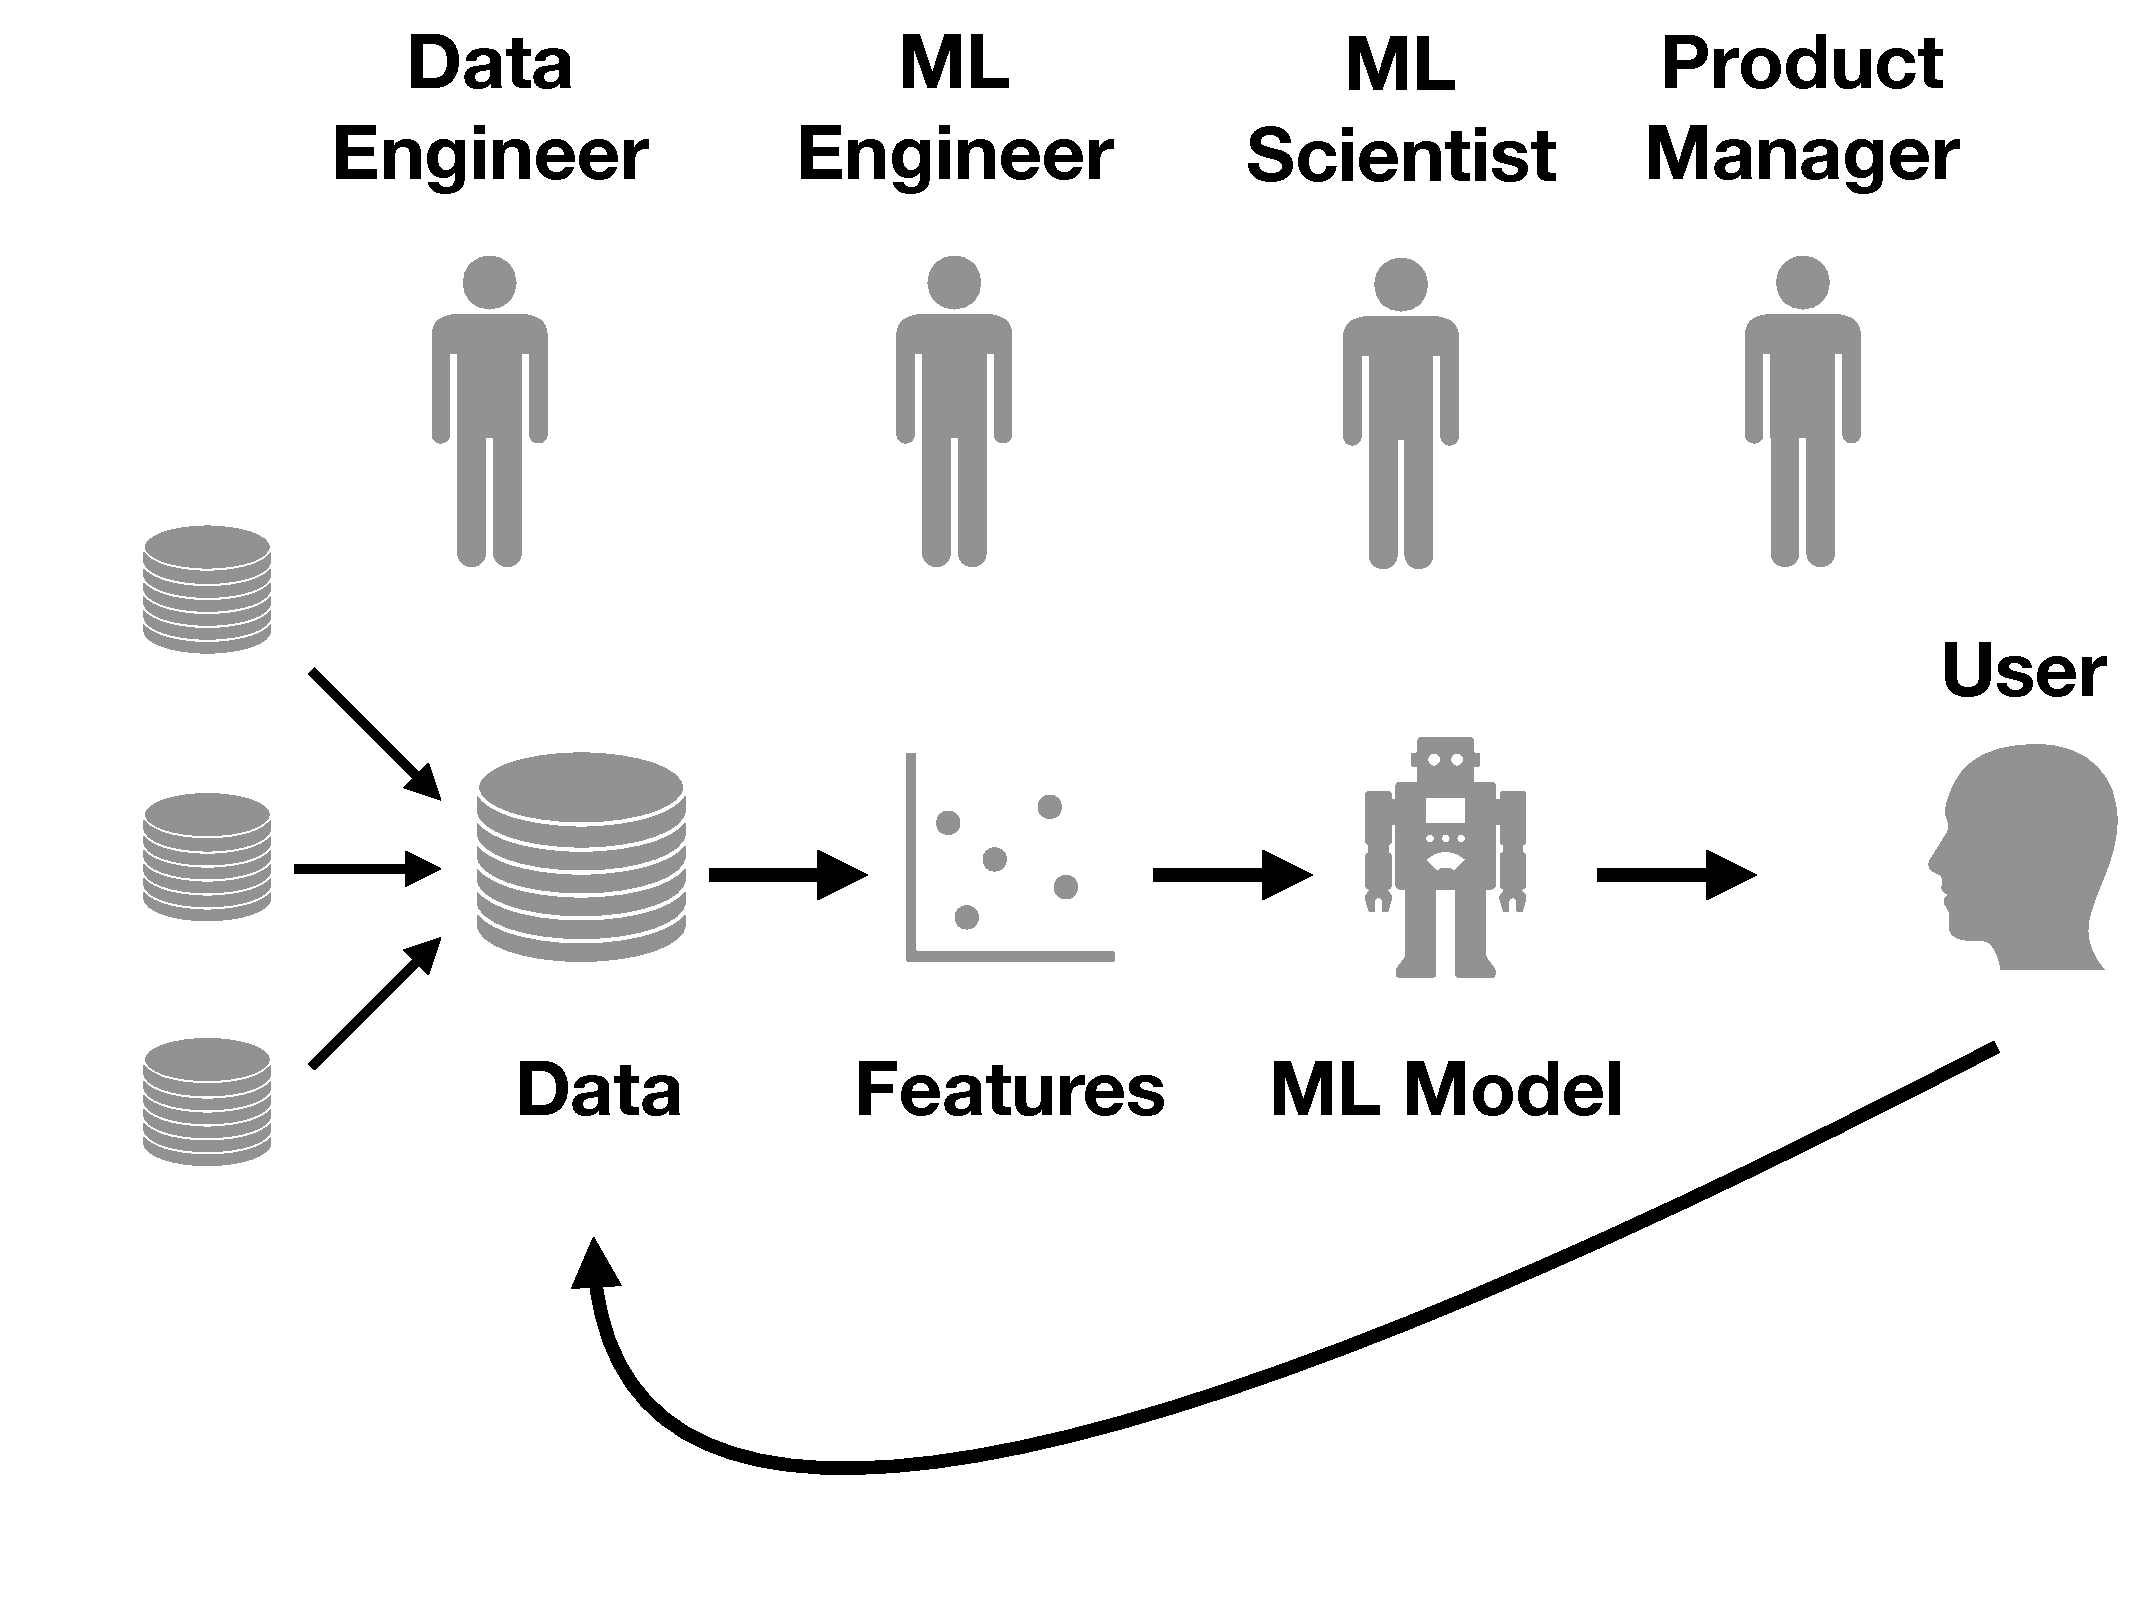
\includegraphics[width=.6\textwidth]{submissions/data-validation-amazon/figs/ML-system}
\caption{Responsibilities for a machine learning (ML) production software system are often distributed across different roles and teams \cite{Polyzotis2018}. Data from various sources is integrated, features are extracted and ML models transform these into predictions, which are then served to users whose behavioural signals are fed back to the system. Monitoring and validating these data streams at scale is only feasible with automated tests. But validating the data in each of these stages requires different competencies and often domain expertise. This imposes novel technical and conceptual challenges on engineering teams when automating ML production systems.}
\label{fig:ml-system}
\end{figure}


But why is this so difficult to automate? Researchers in the DBMS community have been investigating data profiling for decades \cite{Abedjan2018} and many of these solutions are just right for some aspects of data validation also in the context of ML systems. However some of the challenges in ML system monitoring go beyond that. Many data validation aspects in ML systems {\em depend on the state of the trained ML model}, such as the performance of a ML model under data set shift, or the differential privacy of a model \cite{Dwork08differentialprivacy, Abadi2016, Bagdasaryan2019}. Other aspects such as fairness of a ML model require domain expertise that ML engineers often do not have. As illustrated in \autoref{fig:ml-system} the competencies required to validate data in the various stages of an ML system require competencies that are usually distributed across several experts in a team or even separate teams. 

In the following chapters we will first review the challenges associated with data validation in ML systems and highlighting some of the practical implications. Afterwards we review some of the data validation solutions, with a special focus on the practical applicability of these approaches. Finally we will conclude with an outlook of technical and non-technical challenges associated with ML system validation in order to ensure more responsible usage of ML systems in production software systems. 
%!TEX root = data-validation-ml-systems.tex
\section{Data Validation Dimensions}
\label{sec:dimensions}

As ML systems learn from data, validation of the data ingested during training and prediction is a fundamental prerequisite for well functioning and robust ML systems \cite{Sculley2015, Bose2017a}. Relevant data validation dimensions for ML systems can be broadly categorized into those notions of data quality commonly considered in classical data base management systems (DBMS) and ML model dependent dimensions. In the following, we highlight some of the dimensions and provide examples for each category.

\subsection{Classical DBMS dimensions}

Independent of ML applications there are many data validation dimensions that have been investigated in the DBMS community, more specifically in the data profiling literature\cite{Abedjan2018}:

\paragraph{Data Correctness:} This dimension refers to schema violations, such as string values in numeric columns, or generally syntactically wrong data. Defects in this dimension can often break ML processing pipelines. Some of these violations can be detected easily for instance by type checks, and corrupted data instances can be filtered out.


\paragraph{Data Consistency} refers to defects that are not captured by syntactic correctness, including duplicate entries or invalid values. Detecting these cases can be difficult and computationally challenging, but there exist efficient approaches to de-duplication and detection of semantic inconsistencies. Violations of semantic inconsistencies can for instance be detected by validation of functional or approximate functional dependencies \cite{Papenbrock2015, Kruse2018}.

\paragraph{Completeness} of a data source reflects the ratio of missing values in a data set. In principle this dimension is simple to probe, however only under the assumption that the missing value symbol is known. Unfortunately this assumption is often violated. As missing values often cause problems in data pipelines feeding into ML systems, a common strategy of avoid such problems is to replace missing values with syntactically valid values. These transformations often make the missing values pass validations for correctness and consistency.

\newpage
\paragraph{Statistical Properties:} This dimension includes basic descriptive statistics of an attribute, such as mean of a numeric or mode of a categorical variable, and more complex parametric or non-parametric statistical aggregates of a data set. A popular validation strategy in this data dimension is anomaly detection.

\subsection{ML model dependent dimensions}

Validating the above data quality dimensions can be challenging, but these tests of the input data are independent of the downstream ML model. This implies that testing only for these dimensions can lead to both false negatives, when a data corruption is not detected that has a negative impact on the downstream ML model, as well as false positives, when a data corruption raises an alarm but does not have any effect on the downstream ML model. Examples for false negatives of ML model independent validations include adversarial attacks, such as for instance avoiding filters for adult language by {\em leet speak}\footnote{\url{https://en.wikipedia.org/wiki/Leet}} strings obfuscated by misspellings and replacing letters with numeric characters. Examples for false positive alarms are ML models employing strong $L_1$ or sparsity-enforcing regularization constraints. In these models, a large number of input features is often not affecting the ML model output, hence distributional shifts in these input features would not be reflected in shifts of the ML model outputs and validation of the input data independent of the model outputs will raise false alarms.

Data validation in the context of ML production systems thus has to take into account the current state of the downstream ML model to ensure robust and reliable performance. The state of the ML model and and the impact of data corruptions on ML performance can be monitored by a number of different validation dimensions of the ML model {\em output} data. These have to be validated along with the usual criteria common to all production software systems, such as requirements on the latency and availability of the system. SageMaker Model Monitor\footnote{\url{https://docs.aws.amazon.com/sagemaker/latest/dg/model-monitor.html}} is a solution that enables monitoring of models deployed in production. For example, alarms are triggered when data distributions shifts are detected.

\paragraph{Predictive performance metrics} are usually the most important metrics optimized in production ML systems. These metrics include accuracy, precision or F1-score of a classifier, the mean-squared error, mean absolute error or $r^2$-scores for regression models or various ranking losses, evaluated via cross-validation on a test set that was not used for training the respective ML model. When the data processed by  trained and deployed ML model is drawn from the same distribution as the training and test data, then these cross-validated metrics reflect the predictive performance reliably. But in production ML systems, this assumption is often violated. Examples include shifts in the input data (covariate shifts) or shifts in the target data distribution (label shift).

\paragraph{Robustness}
The shifts induced by corruptions in the data that are a) not caught by upstream classical data validation techniques and that have b) a negative impact on the predictive performance of a production ML system can be difficult to detect, as there is no ground truth label information available for the data. In the absence of ground truth data needed to compute predictive performance metrics, one can resort to classical data validation techniques applied to the outputs of ML models. But this approach can fail to detect certain covariate shifts induced by outliers, adversarial attacks or other corruptions.

\paragraph{Privacy metrics} have become increasingly important since ML models are used to process personal data such as health care data, financial transactions, movement patterns or really almost every aspect of our lives. Popular concepts include {\em differential privacy} \cite{Dworak_2006_diff} and {\em k-anonymity} \cite{Sweeney2002}. Note that k-anonymization~\cite{Sweeney2002} is not model dependent, it is a property of a data base where user data is considered private if information about each user cannot be distinguished from at least k-1 other users whose information is in the dataset.
In the field of ML, differential privacy is more useful than k-anonymity. Two main reasons for that are a) k-anonymity is defined for a fixed data set, if new rows are added, one might need to convert the data again in order to achieve k-anonymity, and b) if a k-anonymous data set is combined with other information, it is often possible to de-anonymize the data.
%
A large body of literature in the ML community builds upon the definition of $\epsilon$-differential privacy~\cite{Dworak2014differantial} which deals with the problem of learning little to nothing about individual data-points while learning a lot about the population by ensuring the same conclusions can be drawn whether any single data-point is included in the dataset or not. Most implementations of differentially private ML models add noise to the data, gradients or the model coefficients~\cite{Abadi2016, Shokri2017, papernot2016semisupervised, Mironov2017}. This can be an effective countermeasure to model inversion attacks~\cite{Fredrikson2015} or membership inference attacks \cite{Shokri2017}. The amount of noise added determines the amount of privacy preserved -- but it also bounds the predictive performance or {\em utility} of the ML model \cite{Jayaraman2019}.

\paragraph{Robustness to adversarial data} Recent developments have shown that ML models, placed at the centre of security-critical systems such as self-driving cars, can be targeted by dedicated adversarial examples - inputs that are very difficult to distinguish from regular data but are misclassified by the model~\cite{goodfellow2014explaining}. Those inputs, created by applying a small but very significant perturbation to regular examples can be used to manipulate the model to predict outputs desired by an adversary~\cite{szegedy2013intriguing, Biggio_2013, Nguyen_2015}. The robustness to adversarial attacks of the model can be measured by (1) generating a set of adversarial examples based on the test set~\cite{szegedy2013intriguing, Kurakin2017AdversarialEI, Hosseini2019AreOR, MoosaviDezfooli2016DeepFoolAS, goodfellow2014explaining} and (2) computing what is the change in models accuracy given a fixed average distortion, or what is the minimum average distortion needed to reach 0\% accuracy on the test set.


\paragraph{Fairness}
Another dimension that is highly relevant when putting ML systems in production is that of fairness or more generally ethical aspects of ML predictions \cite{Mehrabi2019}. There are a number of examples when ML technology used as assistive technology for instance in border control\footnote{\url{https://www.bbc.com/news/technology-53650758}} or policing\footnote{\url{https://www.nytimes.com/2019/07/10/opinion/facial-recognition-race.html}} led to racist or otherwise biased decisions. It has been widely recognized in the ML research community that when building ML applications validating the ML predictions with respect to fairness is a fundamental prerequisite. Evaluating this dimension is however amongst the most difficult of all validation  challenges: there are different fairness definitions, and even if one could agree on a small set of definitions, validating these requires insight into the respective grouping variables, which are, for ethical and legal reasons, typically not available. The relevant grouping information is thus often reflected in a data set through other features, which are considered not ethically problematic, such as zip code, but which are often correlated with ethically sensitive features. Other implicit biases of data sets can emerge from data preprocessing, for instance how missing values are dealt with when they are distributed not equally across ethnical groups \cite{Yang2020}. Detecting these biases requires not only domain expertise, but also often information that is not contained in the data set itself.



%
%\begin{enumerate\
%
%\item Classical DBMS dimensions
%\begin{enumerate}
%\item Correctness (e.g. Unknown schemas / data types, Wrong entries)
%\item Consistency (e.g. Duplicates, Invalid values)
%\item Statistical properties (Anomalies, Are value distributions changing over time? Is a column predictable from another column?)
%\item Completeness (How many missing values?)
%\end{enumerate}

%\item ML model dependent dimensions
%\begin{enumerate}
%\item Generalization performance
%\item Performance under (covariate, label) shift
%\item Performance for single (rare) classes
%\item Performance for single subgroups ({\bf fairness})
%\item Robustness to adversarial data
%\item Differential privacy
%\item Constraints on compute time (some data points could lead to long prediction times, e.g. due to lack of sparsity)
%\end{enumerate}
%\end{enumerate}

%!TEX root = data-validation-ml-systems.tex
\section{Current Solutions}
\label{sec:solutions}

Validating data at each of the stages in a ML workflow as sketched in \autoref{fig:ml-system} requires a wide range of competencies from data engineering over ML algorithms to user interface design. These competencies are often distributed across different roles in a team, and especially in small (5 to 10 members) teams, it is not unlikely that only one person has the competency to dive deep into a root cause analysis of the various data validation dimensions sketched in \autoref{sec:dimensions}. Solving problems in an on-call situation or when scaling up an ML system requires reliable automation for the data validation. As many of these validations have to be data dependent, such automation often amounts to {\em using ML to validate data in ML workflows} which has, for instance, been done for outlier removal \cite{Zhao2019}, data cleaning \cite{Krishnan2019} or missing value imputation \cite{Biessmann2018a}. 

\newpage
There are, however, simpler approaches that do not leverage ML models to validate data in ML systems, such as Tensorflow Extended (TFX) \cite{Baylor2017} or DEEQU \cite{Schelter2018}. In the following we will highlight some of the state of the art solutions to automated data validation in the context of ML systems.


\subsection{Schema Validation}

Validating syntactic correctness, also referred to as schema validation, is -- at first glance -- relatively simple and often integral part of data ingestion. Usually data violating data type constraints will immediately raise errors and break a data pipeline. Yet, these validations are often counteracted by humans. In practice it is not uncommon to use generic data types such as strings for data that is actually numeric, ordinal or categorical. While this will ensure that schema violations are minimized, as any data type can be cast to string, it imposes additional work on any downstream validation for data correctness and consistency. This problem is worsened by the fact that some software libraries popular in the ML community often cast string data that contains numeric data automatically to numeric data types. This can have effects on entire scientific communities. A recent study reports that casting errors induced by excel in biomedical data occur in approximately one fifth of the papers in leading genomics journals \cite{Ziemann2016}.

While simple validation such the data type can be trivially automated, it is unlikely that this will prevent engineers from having to deal with data type errors. There will always be on-call engineers who need to fix problems as fast as possible and the cost of having stale or broken data pipelines in a production system is often far bigger then the difficulty to quantify cost of accumulating hidden technical debt by specifying generic data types like strings and thereby circumventing data type checks. This is why this simple task of data type detection is actually an interesting research challenge. Often simple heuristics will do the job and the popular libraries use these heuristics to determine the data type of columns. The simplest heuristic is probably to try and cast a value to a certain data type and try other data types in case an error is raised\footnote{\url{https://github.com/pandas-dev/pandas/blob/v1.1.4/pandas/core/dtypes/common.py\#L138}}. Such heuristics often work well in practice but can be insufficient, especially when dealing with heterogeneous data, such as mixed data types in one column. Also, for the seemingly simple task of automating data type inference, there is interesting recent work on using ML models to infer a probabilistic notion of the most likely data type given the symbols used in a data base~\cite{Ceritli2020}. Approaches combining scalable heuristics with more sophisticated ML based data type inference techniques are a promising alternative to the current situation in which restrictive data type checks and broken data pipelines often lead data engineers to opt for too generic data types.

\subsection{Data Correctness and Data Consistency}

Validation of data consistency and correctness are one of the areas where classical DBMS research has made significant contributions, for instance in the data profiling literature \cite{Abedjan2018}. Popular approaches to validate correctness and consistency are rule based systems such as {\em NADEEF} \cite{Dallachiesat2013}. There are commercial versions of simple rule based systems, a popular example is trifacta\footnote{\url{https://www.trifacta.com/}}. And there are open source systems for semi-automated validation of consistency, such as Open-Refine\footnote{\url{https://openrefine.org/}}. Other approaches primarily investigated in an academic context include attempts to learn {\em (approximate/relaxed) functional dependencies} between columns of a table \cite{Papenbrock2015}. These functional dependencies between columns include for example a dependency between a column containing zip codes and another column containing city names. These dependencies can be used to automatically learn validation checks related to consistency and correctness \cite{Rekatsinas2017}. Such approaches are well established and there exist efficient methods for large scale functional dependency discovery \cite{Kruse2018}. Yet, in the context of data pipelines for ML systems none of these approaches have reached broad adoption. We discuss some potential reasons in \autoref{sec:conclusion}.

In addition to the solutions of the DBMS community there are a number of approaches developed at the intersection of DBMS and ML  communities, tailored to ML specific workflows \cite{Breck2019, Schelter2018}. The research is accompanied by open source libraries\footnote{\url{https://www.tensorflow.org/tfx/guide/tfdv}}\footnote{\url{https://github.com/awslabs/deequ}} that implement schema validation by checking for correct data types, but they also offer validation options for or other basic data properties, for instance whether the values are contained in a predefined set. Prominent examples for a data validation solution for ML systems are the ones integrated in SageMaker Data Wrangler\footnote{\url{https://aws.amazon.com/sagemaker/data-wrangler/}} and TFX \cite{Breck2019}. Their schema validation conveniently allows users to define integrity checks on the serving data in an ML system, e.g. for data type or value ranges. Schema validation parameters can also be derived from the training data, which allows to automate many of these checks.

\subsection{Validation of Statistical Properties}

All data sets are subject to noise, be it because humans enter wrong values into a form or because human software developers write code that leads to faulty data ingestion. Dealing with this noise is difficult for exact validation rules such as functional dependencies. Statistical learning techniques can help to deal with noisy data.

\paragraph{Error-Detection Solutions}
Taking a probabilistic stance on DBMSs is not a new idea \cite{Cavallo1987}. Recently, the idea of using statistical techniques for data validation tasks has become a major focus of research. One example are statistical learning approaches to error detection in data bases \cite{Rekatsinas2017,Heidari2019,Huang2017,MahdaviBerlinmahdavilahijani}. These approaches have the potential to automatically validate data correctness and to automatically clean data sets. Some of these systems can be automated to a large extent \cite{Krishnan2017, Krishnan2019}, others rely on a  semi-supervised approach \cite{Krishnan:2016b}.

\paragraph{ML Frameworks for Statistical Data Validation}
Also data validation solutions like TFX data validation \cite{Breck2019} or DEEQU \cite{Schelter2018} address data validation including statistical rules, such as deviation of values around the mean of a numeric column. These validation solutions can be very helpful, if one knows what to test for. But data sources can easily have billions of rows and hundreds of columns. For these cases it can infeasible to manually create, validate and maintain data quality checks. To alleviate the burden of manually creating constraints, the authors of DEEQU \cite{Schelter2018} propose to utilize historic data to generate column profiles and generate data quality constraints from these. These quality constraints can also make use of the temporal structure of data quality metrics collected over time using time series models or other anomaly detection methods.

\paragraph{Anomaly Detection Methods}
Instead of applying them to metrics computed on a data set, anomaly detection methods are also often used to detect anomalies in the data tuples directly. There are many methods available in easy to use software libraries, see for instance \cite{Zhao2019}, and there are commercial products that allow to automate anomaly detection in large scale industrial settings\footnote{\url{https://aws.amazon.com/de/blogs/big-data/real-time-clickstream-anomaly-detection-with-amazon-kinesis-analytics/}}. While the goal of these anomaly detection approaches is similar to the above error detection approaches originating in the DBMS community, many anomaly detection solutions emerged from the ML community. One of the most important differences is that anomaly detection approaches, as most ML methods, usually expect the data to come in matrix form, with all columns being numeric. Most methods from the DBMS community expect the data to be high cardinality categorical data, some also are applicable to numeric values, but that is not very common in research on functional dependencies for instance \cite{Papenbrock2015}. So applying anomaly detection methods to heterogeneous data sets with non-numeric (categorical, ordinal or even free text data) requires to apply {\em feature extraction} techniques to bring the data into a numeric format. This is a standard preprocessing step in ML pipelines, but popular software libraries for anomaly detection, such as  \cite{Zhao2019}, do not include this important preprocessing step. This makes these libraries difficult to apply for automated data validation. It is possible to integrate standard anomaly detection methods as statistical data validation steps in ML systems, but this imposes two additional challenges onto the engineering team. For one, this integration requires to write 'glue code' for the feature extraction -- which is often one of the major sources for accumulating {\em technical debt} in a software system. And secondly this requires to have a good evaluation metric for the anomaly detection. Which is, in contrast to standard supervised learning scenarios, often difficult to define and get ground truth data for.

\paragraph{Model Robustness and Generalization Performance}
Another central problem with all of the above approaches to statistical data validation in a ML context is that most of these methods are blind to the impact of data errors on downstream ML components. This is however one of the most important aspects for ML systems. Often it does not matter for the ML model, whether a feature is affected by a data shift, for instance when regularization of an ML model forces the ML model to ignore a feature. And in other cases tiny changes in the input, which human observers would not be able to detect, can have devastating consequences on the ML model output \cite{Athalye18}. Recent work in the ML community has shown that especially novel deep learning methods can suffer from severe stability problems \cite{DAmour2020}. Some aspects of this can be mitigated by employing standard ML concepts such as k-fold cross-validation (CV). This approach has unfortunately lost popularity due to the sheer compute demand of modern deep learning methods. Most deep learning papers usually use just a single train/validation/test split. Standard nested k-fold CV can have decisive advantages when it comes to measuring robustness of a ML model. However, these techniques only work when there is ground truth data available. In a production setting, this is often not the case. There exist however also other methods to measure the robustness of ML models when there is no ground truth data available. For instance in \cite{Schelter2020} the authors leverage a set of declaratively defined data errors applied to data for which ground truth is available and measure the predictive performance of a ML model under these perturbations. This allows to train a meta model that can be used to predict the predictive performance on new unseen data with high precision. Such an approach can be useful in production ML systems to automatically validate data errors with respect to their impact on downstream ML model performance.

\subsection{Fairness Validation}

Fairness is one of the most prominent examples of how ML systems can fail and severely influence the public opinion about a company or an entire scientific community. It is thus of utmost importance to ensure that this dimension of data validation in the context of ML systems is not neglected. Yet validating this dimension is especially difficult, for a number of reasons. First and foremost it is difficult to define fairness. An excellent overview over the last decades of fairness research with a focus on ML systems can be found in \cite{Mehrabi2019}. The main insight here is that fairness validation it is not only a technical challenge. Instead, it is imperative to include multiple scientific disciplines in this research, in particular also researchers from sociology, psychology and law. Setting the stage for such transdisciplinary research is a challenge in itself, for instance finding a common terminology is not trivial. But we have seen that the research community has made progress by fostering transdisciplinary discussions at newly emerging conferences\footnote{See for instance \url{https://dl.acm.org/conference/fat}}. The joint efforts of different communities have helped to identify many ways in which biases leading to unfair ML systems can enter a workflow. Many of these biases arise in the data generating process. Enabling scientists and engineers to identify such biases should be part of the research agenda of the data management and ML community \cite{Stoyanovich2020}. One example in this direction is {\em FairBench}~\cite{Yang2020}, an open source library that helps to trace changes in data distributions and visualize distortions with respect to protected group memberships throughout the pipeline. Another example is SageMaker Clarify\footnote{https://aws.amazon.com/sagemaker/clarify/}, an explainability feature for Amazon SageMaker that provides insights into data and ML models by identifying biases and explaining predictions. It is deeply integrated into Amazon SageMaker, a fully managed service that enables data scientists and developers to build, train, and deploy ML models at any scale. Clarify supports bias detection and feature importance computation across the ML lifecycle, during data preparation, model evaluation, and post-deployment monitoring. Libraries like these  are a prerequisite to better automation of fairness validation.
%
However, another more fundamental problem of fairness validation remains even if technical solutions for visualizing and detecting biases are available: Group membership variables are required for most technical solutions to fairness. Storing these variables can
be more challenging, from an operational stance, than storing other non-confidential data.


\subsection{Privacy Validation}
Similar to fairness, also privacy is a difficult to define validation dimension. However in contrast to fairness, the research community has converged to a few concepts that are relatively straightforward in terms of their definitions. Popular concepts include {\em differential privacy} \cite{Dworak_2006_diff} and {\em k-anonymity} \cite{Sweeney2002}, see also \autoref{sec:dimensions}.
Most ML related work on privacy focuses on differential privacy, where noise is added the data, gradients or the model coefficients. Validating and trading off privacy against predictive performance or {\em utility} of the ML model can be challenging \cite{Jayaraman2019}.
Empirically, evaluating privacy is often done using {\em membership inference attacks} \cite{Shokri2017}, which has also been adopted for unsupervised ML models \cite{Hayes2019}. One limitation of these approaches is that privacy validation is always dependent on a specific model and data set. General statements about privacy and utility independent of models and data is hence difficult.

\subsection{Validation of Robustness against adversarial attacks}

Privacy validation is aiming at defending the ML system against a certain type of adversarial attack, where for instance the identity of data points used for training the ML system is revealed. There are however other types of adversarial attacks, for instance when artificial examples are generated to result in ML predictions with a certain outcome. Validation of robustness against such types of attacks can be achieved by perturbations around the data manifold~\cite{pang2017robust, aleks2017deep}. This can be achieved by extracting latent representations of the input data~\cite{hendrycks2016early} or of the predictions~\cite{Bhagoji_2018, feinman2017detecting}. Alternative methods rely on training an additional classifier used to decide whether an example is adversarial or not~\cite{gong2017adversarial, grosse2017statistical, metzen2017detecting}. Complementary to the work on validating adversarial robustness, a lot of work has been devoted to making ML models more robust to adversarial attacks by augmenting the training datasets with adversarial examples~\cite{goodfellow2014explaining,aleks2017deep, zhang2019, Dingyuan2019}.


\subsection{Human in the loop evaluation}

Most of the above data quality dimensions are easy for humans to assess. This is why human audits are still one of the most direct and most robust options for data validation in ML systems. Expert auditors, such as researchers developing a new service, often can quickly identify errors and their root causes by simply inspecting input and outputs of a ML system. Among the most important disadvantages with this approach is that these validations are expensive and do not scale well. Sometimes human-in-the-loop validations can be scaled up using crowd-sourcing platforms such as Yandex' Toloka or Amazon Mechanical Turk. Increasing the quality of crowd-sourced validations is an active topic of ML research \cite{WortmanVaughan2018}. For instance there are attempts to render audits more efficient by including transparency of ML model predictions \cite{schmidt2019quantifying} or by providing more inciting incentives~\cite{Ho_2015, wang_2018}. Still, this approach can be difficult to automate and is generally used as an andon cord in a modelling pipeline rather than an integrated quality test. This is not only due to the fact that it is difficult to integrate human audits in build processes. Focussing on human judgements only can lead to biased validations, especially when using transparent ML methods~\cite{schmidt2020risk}.

%!TEX root = data-validation-ml-systems.tex
\section{Conclusion}
\label{sec:conclusion}

Validation of input and output data in ML production systems has many facets that require competencies often distributed across a heterogeneous team of engineers and scientists, as illustrated in \autoref{fig:ml-system}. While some of the data validation challenges, such as schema validation or data consistency, can be tackled with traditional data profiling methods established the DBMS community, other validation dimensions are specific to ML systems. These ML model dependent validation challenges include aspects like accuracy and robustness under data shifts, fairness of ML model predictions and privacy concerns. 

In \autoref{sec:solutions} we highlight a number of solutions to validate single aspects. Many of these approaches are typically tailored to specific use cases and often require considerable integration efforts in production ML systems. 
A good example are the various solutions from both the ML community as well as the DMBS community for checking simple data properties, such as the data types, and also more complex dimensions like data consistency. Many of these approached allow for automating the generation of validation checks. Yet in practice it is not trivial to automate the generation of validations for a new ML system that ingests and produces millions of rows and columns. For instance, there are many cases when simple validation checks on input data will lead to false alarms when shifts or errors in a single feature do not impact the output of a downstream ML model -- maybe because that feature was neglected by the ML model, when strong regularization during the ML model training phase taught the model to ignore that feature. 

Despite the rapid progress in recent years to automate and monitor ML systems: to the best of our knowledge there exists no data validation system that has reached broad adoption and which takes into account all of the data validation dimensions sketched in \autoref{sec:dimensions}. One reason for this is the difficulty of combining the multitude of validation strategies listed in \autoref{sec:solutions} into one unified framework. Considering the rapid pace of research at the intersection of ML and DBMS, see for instance \cite{Dong2018}, it is fair to assume that it is merely a matter of a few years until one framework or some open standard for data validation in the context of ML systems will have reached broad adoption. 

There are many data validation challenges in ML systems that go beyond technical aspects. Many of them are due to the complex nature of the data transformations induced by ML models. For instance identifying unfair biases often requires domain knowledge or access to grouping variables, which are often not available. And even if those are available, it is not always clear how fairness in the context of ML systems can be defined  \cite{Zhang2020}. A conceptual challenge related to privacy is for instance the trade-off between utility and differential privacy of a ML system \cite{Jayaraman2019}: how much predictive accuracy should be sacrificed to ensure privacy? Sacrificing accuracy against privacy in domains like health care or jurisdiction is a difficult question for which ethical and legal dimensions are more important than technical aspects. Next to these ethical and legal aspects, there is one key factor hindering adoption of comprehensive data validation in ML systems and that more related to cultural aspects. Many scientists like to build new models and tools, but writing tests, integrating monitoring and validation stages in an ML system are not exactly the most popular tasks amongst researchers. But often the competencies of the scientists who built a model is required to build well functioning monitoring and validation solutions in ML systems. 

Based on these observations we derive some suggestions for how to drive innovation and adoption of data validation in the context of ML systems. First, we hope that the current trend for research at the intersection of ML and DBMS communities will continue to grow and identify more synergies leveraging and complementing each others expertise. We have seen some great examples of constructive but vivid discussion between the two communities, for instance that sparked by Kraska and colleagues around their work on learning index structures \cite{Kraska2018}. This work is unrelated to data validation and mentioned merely as an example of transdisciplinary research debates. 
Second, when building ML systems there is a broad spectrum of operational challenges and seamless integration with cloud infrastructure is key to reaching broad adoption. 

\newpage
We conclude that establishing data validation in ML systems will require a stronger focus on usability and simple APIs. Third we believe that data validation in ML systems will reach broad adoption once the research community will have found better ways of automating the validation workflow, most importantly the generation of checks for each of the data validation dimensions listed in \autoref{sec:dimensions}. 

In the past years we have seen great examples of automated tooling for tracking ML experiments \cite{Schelter2017}, experimentation in ML production systems \cite{Bose2017a}, input data validation \cite{Schelter2018,Breck2019} and validation strategies for predictions of ML systems \cite{Rabanser2018,Schelter2020,DAmour2020}. One example of how some of these data validation techniques could be integrated into an automated workflow would be that presented in \cite{Rukat2020}, where the authors propose to iterate through a sequence of data validation~\cite{Schelter2018}, data cleaning\cite{Biessmann2018a} and quantification of downstream impact on ML predictive performance~\cite{Schelter2020} to achieve an automated ML workflow. We believe that increasing the level of usability through automation in data validation will enable researchers to focus on more important questions like the conceptual, ethical and legal questions and ultimately lead to more responsible usage of ML systems in production systems.


%\begin{small}
%	\bibliographystyle{plain}
%	\bibliography{data-validation-ml-systems}
%\end{small}


\begin{thebibliography}{10}

\bibitem{Polyzotis2018}
{\em {Data Lifecycle Challenges in Production Machine Learning: A Survey}},
  number (Vol. 47, No. 2). SIGMOD Record, 2018.

\bibitem{Abadi2016}
Martin Abadi, Andy Chu, Ian Goodfellow, H.~Brendan McMahan, Ilya Mironov, Kunal
  Talwar, and Li~Zhang.
\newblock Deep learning with differential privacy.
\newblock In {\em Proceedings of the 2016 ACM SIGSAC Conference on Computer and
  Communications Security}, CCS '16, pages 308--318, New York, NY, USA, 2016.
  Association for Computing Machinery.

\bibitem{Abedjan2018}
Ziawasch Abedjan, Lukasz Golab, Felix Naumann, and Thorsten Papenbrock.
\newblock {Data Profiling}.
\newblock {\em Synthesis Lectures on Data Management}, 10(4):1--154, nov 2018.

\bibitem{Athalye18}
Anish Athalye, Logan Engstrom, Andrew Ilyas, and Kevin Kwok.
\newblock Synthesizing robust adversarial examples.
\newblock volume~80 of {\em Proceedings of Machine Learning Research}, pages
  284--293, Stockholmsm{\"a}ssan, Stockholm Sweden, 10--15 Jul 2018. PMLR.

\bibitem{Bagdasaryan2019}
Eugene Bagdasaryan, Omid Poursaeed, and Vitaly Shmatikov.
\newblock Differential privacy has disparate impact on model accuracy.
\newblock In H.~Wallach, H.~Larochelle, A.~Beygelzimer, F.~Alch\'{e}-Buc,
  E.~Fox, and R.~Garnett, editors, {\em Advances in Neural Information
  Processing Systems}, volume~32, pages 15479--15488. Curran Associates, Inc.,
  2019.

\bibitem{Baylor2017}
Denis Baylor, Eric Breck, Heng~Tze Cheng, Noah Fiedel, Chuan~Yu Foo, Zakaria
  Haque, Salem Haykal, Mustafa Ispir, Vihan Jain, Levent Koc, Chiu~Yuen Koo,
  Lukasz Lew, Clemens Mewald, Akshay~Naresh Modi, Neoklis Polyzotis, Sukriti
  Ramesh, Sudip Roy, Steven~Euijong Whang, Martin Wicke, Jarek Wilkiewicz, Xin
  Zhang, and Martin Zinkevich.
\newblock {TFX: A TensorFlow-based production-scale machine learning platform}.
\newblock In {\em Proceedings of the ACM SIGKDD International Conference on
  Knowledge Discovery and Data Mining}, volume Part F129685, pages 1387--1395,
  New York, NY, USA, aug 2017. Association for Computing Machinery.

\bibitem{Bhagoji_2018}
Arjun~Nitin Bhagoji, Daniel Cullina, Chawin Sitawarin, and Prateek Mittal.
\newblock Enhancing robustness of machine learning systems via data
  transformations.
\newblock {\em 2018 52nd Annual Conference on Information Sciences and Systems
  (CISS)}, Mar 2018.

\bibitem{Biessmann2018a}
Felix Biessmann, David Salinas, Sebastian Schelter, Philipp Schmidt, and Dustin
  Lange.
\newblock {"Deep" Learning for Missing Value Imputationin Tables with
  Non-Numerical Data}.
\newblock In {\em Proceedings of the 27th ACM International Conference on
  Information and Knowledge Management - CIKM '18}, pages 2017--2025, New York,
  New York, USA, 2018. ACM Press.

\bibitem{Biggio_2013}
Battista Biggio, Igino Corona, Davide Maiorca, Blaine Nelson, Nedim {\v
  S}rndi{\'c}, Pavel Laskov, Giorgio Giacinto, and Fabio Roli.
\newblock Evasion attacks against machine learning at test time.
\newblock {\em Lecture Notes in Computer Science}, pages 387--402, 2013.

\bibitem{Bose2017a}
Joos~Hendrik B{\"{o}}se, Valentin Flunkert, Jan Gasthaus, Tim Januschowski,
  Dustin Lange, David Salinas, Sebastian Schelter, Matthias Seeger, and Yuyang
  Wang.
\newblock {Probabilistic demand forecasting at scale}.
\newblock {\em Proceedings of the VLDB Endowment}, 10(12):1694--1705, 2017.

\bibitem{Breck2019}
Eric Breck, Neoklis Polyzotis, Sudip Roy, Steven~Euijong Whang, and Martin
  Zinkevich.
\newblock {DATA VALIDATION FOR MACHINE LEARNING}.
\newblock Technical report, 2019.

\bibitem{Ceritli2020}
Taha Ceritli, Christopher~K.I. Williams, and James Geddes.
\newblock ptype: probabilistic type inference.
\newblock {\em Data Mining and Knowledge Discovery}, 34(3):870--904, may 2020.

\bibitem{Dallachiesat2013}
Michele Dallachiesat, Amr Ebaid, Ahmed Eldawy, Ahmed Elmagarmid, Ihab~F. Ilyas,
  Mourad Ouzzani, and Nan Tang.
\newblock {NADEEF: A commodity data cleaning system}.
\newblock In {\em Proceedings of the ACM SIGMOD International Conference on
  Management of Data}, 2013.

\bibitem{DAmour2020}
Alexander D'Amour, Katherine Heller, Dan Moldovan, Ben Adlam, Babak Alipanahi,
  Alex Beutel, Christina Chen, Jonathan Deaton, Jacob Eisenstein, Matthew~D.
  Hoffman, Farhad Hormozdiari, Neil Houlsby, Shaobo Hou, Ghassen Jerfel, Alan
  Karthikesalingam, Mario Lucic, Yian Ma, Cory McLean, Diana Mincu, Akinori
  Mitani, Andrea Montanari, Zachary Nado, Vivek Natarajan, Christopher Nielson,
  Thomas~F. Osborne, Rajiv Raman, Kim Ramasamy, Rory Sayres, Jessica Schrouff,
  Martin Seneviratne, Shannon Sequeira, Harini Suresh, Victor Veitch, Max
  Vladymyrov, Xuezhi Wang, Kellie Webster, Steve Yadlowsky, Taedong Yun,
  Xiaohua Zhai, and D.~Sculley.
\newblock {Underspecification Presents Challenges for Credibility in Modern
  Machine Learning}.
\newblock 2020.

\bibitem{Dong2018}
Xin~Luna Dong and Theodoros Rekatsinas.
\newblock {Data Integration and Machine Learning: A Natural Synergy}.
\newblock {\em Proceedings ofthe VLDB Endowment, Vol.}, 11(12):2094--2097,
  2018.

\bibitem{Dwork08differentialprivacy}
Cynthia Dwork.
\newblock Differential privacy: A survey of results.
\newblock In {\em In Theory and Applications of Models of Computation}, pages
  1--19. Springer, 2008.

\bibitem{Dworak_2006_diff}
Cynthia Dwork, Frank McSherry, Kobbi Nissim, and Adam Smith.
\newblock Calibrating noise to sensitivity in private data analysis.
\newblock In Shai Halevi and Tal Rabin, editors, {\em Theory of Cryptography},
  pages 265--284, Berlin, Heidelberg, 2006. Springer Berlin Heidelberg.

\bibitem{Dworak2014differantial}
Cynthia Dwork and Aaron Roth.
\newblock The algorithmic foundations of differential privacy.
\newblock {\em Found. Trends Theor. Comput. Sci.}, 9(3--4):211--407, August
  2014.

\bibitem{feinman2017detecting}
Reuben Feinman, Ryan~R. Curtin, Saurabh Shintre, and Andrew~B. Gardner.
\newblock Detecting adversarial samples from artifacts, 2017.

\bibitem{Fredrikson2015}
Matt Fredrikson, Somesh Jha, and Thomas Ristenpart.
\newblock {Model inversion attacks that exploit confidence information and
  basic countermeasures}.
\newblock In {\em Proceedings of the ACM Conference on Computer and
  Communications Security}, 2015.

\bibitem{gong2017adversarial}
Zhitao Gong, Wenlu Wang, and Wei-Shinn Ku.
\newblock Adversarial and clean data are not twins, 2017.

\bibitem{goodfellow2014explaining}
Ian~J. Goodfellow, Jonathon Shlens, and Christian Szegedy.
\newblock Explaining and harnessing adversarial examples, 2014.

\bibitem{grosse2017statistical}
Kathrin Grosse, Praveen Manoharan, Nicolas Papernot, Michael Backes, and
  Patrick McDaniel.
\newblock On the (statistical) detection of adversarial examples, 2017.

\bibitem{Hayes2019}
Jamie Hayes, Luca Melis, George Danezis, and Emiliano~De Cristofaro.
\newblock {LOGAN: Membership Inference Attacks Against Generative Models}.
\newblock {\em Proceedings on Privacy Enhancing Technologies},
  2019(1):133--152, 2019.

\bibitem{Heidari2019}
Alireza Heidari, Joshua McGrath, Ihab~F Ilyas, and Theodoros Rekatsinas.
\newblock {HoloDetect: Few-Shot Learning for Error Detection}.
\newblock {\em ACM Reference Format}, 2019.

\bibitem{hendrycks2016early}
Dan Hendrycks and Kevin Gimpel.
\newblock Early methods for detecting adversarial images, 2016.

\bibitem{Ho_2015}
Chien-Ju Ho, Aleksandrs Slivkins, Siddharth Suri, and Jennifer~Wortman Vaughan.
\newblock Incentivizing high quality crowdwork.
\newblock {\em Proceedings of the 24th International Conference on World Wide
  Web - WWW '15}, 2015.

\bibitem{Hosseini2019AreOR}
H.~Hosseini, S.~Kannan, and R.~Poovendran.
\newblock Are odds really odd? bypassing statistical detection of adversarial
  examples.
\newblock {\em ArXiv}, abs/1907.12138, 2019.

\bibitem{Huang2017}
Zhipeng Huang and Yeye He.
\newblock {Auto-Detect: Data-Driven Error Detection in Tables}.
\newblock {\em SIGMOD}, 2017.

\bibitem{Jayaraman2019}
Bargav Jayaraman and David Evans.
\newblock {\em {Evaluating Differentially Private Machine Learning in
  Practice}}.
\newblock 28th USENIX Security Symposium, 2019.

\bibitem{Kraska2018}
Tim Kraska, Alex Beutel, Ed~H Chi, Jeffrey Dean, and Neoklis Polyzotis.
\newblock {The case for learned index structures}.
\newblock In {\em Proceedings of the ACM SIGMOD International Conference on
  Management of Data}, pages 489--504, 2018.

\bibitem{Krishnan2017}
Sanjay Krishnan, Michael~J Franklin, Ken Goldberg, and Eugene Wu.
\newblock {BoostClean: Automated Error Detection and Repair for Machine
  Learning}.

\bibitem{Krishnan:2016b}
Sanjay Krishnan, Jiannan Wang, Eugene Wu, Michael~J. Franklin, and K.~Goldberg.
\newblock {ActiveClean: Interactive data cleaning for statistical modeling}.
\newblock {\em Proceedings of the VLDB Endowment}, 9(12):948--959, 2016.

\bibitem{Krishnan2019}
Sanjay Krishnan and Eugene Wu.
\newblock {AlphaClean: Automatic Generation of Data Cleaning Pipelines}.
\newblock apr 2019.

\bibitem{Kruse2018}
Sebastian Kruse and Felix Naumann.
\newblock {Efficient Discovery of Approximate Dependencies}.
\newblock {\em PVLDB}, 11(7):759--772, 2018.

\bibitem{Kumar2017}
Arun Kumar, Matthias Boehm, and Jun Yang.
\newblock {Data Management in Machine Learning: Challenges, Techniques, and
  Systems}.
\newblock In {\em SIGMOD}, 2017.

\bibitem{Kurakin2017AdversarialEI}
A.~Kurakin, Ian~J. Goodfellow, and S.~Bengio.
\newblock Adversarial examples in the physical world.
\newblock {\em ArXiv}, abs/1607.02533, 2017.

\bibitem{aleks2017deep}
Aleksander Madry, Aleksandar Makelov, Ludwig Schmidt, Dimitris Tsipras, and
  Adrian Vladu.
\newblock Towards deep learning models resistant to adversarial attacks, 2017.

\bibitem{MahdaviBerlinmahdavilahijani}
Mohammad~TU {Mahdavi Berlin mahdavilahijani}, tu-berlinde {Ziawasch Abedjan},
  Raul {Castro Fernandez MIT}, Samuel {Madden MIT}, Mourad Ouzzani, Michael
  {Stonebraker MIT}, Nan Tang, Mohammad Mahdavi, Ziawasch Abedjan, Raul {Castro
  Fernandez}, Samuel Madden, and Michael Stonebraker.
\newblock {Raha: A Configuration-Free Error Detection System}.
\newblock 18(19).

\bibitem{Mehrabi2019}
Ninareh Mehrabi, Fred Morstatter, Nripsuta Saxena, Kristina Lerman, and Aram
  Galstyan.
\newblock {A Survey on Bias and Fairness in Machine Learning}.
\newblock aug 2019.

\bibitem{metzen2017detecting}
Jan~Hendrik Metzen, Tim Genewein, Volker Fischer, and Bastian Bischoff.
\newblock On detecting adversarial perturbations, 2017.

\bibitem{Mironov2017}
I.~{Mironov}.
\newblock R{\'e}nyi differential privacy.
\newblock In {\em 2017 IEEE 30th Computer Security Foundations Symposium
  (CSF)}, pages 263--275, 2017.

\bibitem{MoosaviDezfooli2016DeepFoolAS}
Seyed-Mohsen Moosavi-Dezfooli, Alhussein Fawzi, and P.~Frossard.
\newblock Deepfool: A simple and accurate method to fool deep neural networks.
\newblock {\em 2016 IEEE Conference on Computer Vision and Pattern Recognition
  (CVPR)}, pages 2574--2582, 2016.

\bibitem{Nguyen_2015}
Anh Nguyen, Jason Yosinski, and Jeff Clune.
\newblock Deep neural networks are easily fooled: High confidence predictions
  for unrecognizable images.
\newblock {\em 2015 IEEE Conference on Computer Vision and Pattern Recognition
  (CVPR)}, Jun 2015.

\bibitem{pang2017robust}
Tianyu Pang, Chao Du, Yinpeng Dong, and Jun Zhu.
\newblock Towards robust detection of adversarial examples, 2017.

\bibitem{Papenbrock2015}
Thorsten Papenbrock, Jens Ehrlich, Jannik Marten, Tommy Neubert, Jan-Peer
  Rudolph, Martin Sch{\"{o}}nberg, Jakob Zwiener, and Felix Naumann.
\newblock {Functional dependency discovery}.
\newblock {\em Proceedings of the VLDB Endowment}, 8(10):1082--1093, jun 2015.

\bibitem{papernot2016semisupervised}
Nicolas Papernot, Mart{\'\i}n Abadi, {\'U}lfar Erlingsson, Ian Goodfellow, and
  Kunal Talwar.
\newblock Semi-supervised knowledge transfer for deep learning from private
  training data, 2016.

\bibitem{Cavallo1987}
Michael Pittarelli.
\newblock {Roger Cavallo}.
\newblock {\em Proceedings of the Thirteenth International Conference on Very
  Large Data Bases}, (January):71--81, 1987.

\bibitem{Rabanser2018}
Stephan Rabanser, Stephan G{\"{u}}nnemann, and Zachary~C Lipton.
\newblock {Failing loudly: An empirical study of methods for detecting dataset
  shift}, 2018.

\bibitem{Rekatsinas2017}
Theodoros Rekatsinas, Xu~Chu, Ihab~F Ilyas, and Christopher R{\'{e}}.
\newblock {HoloClean: Holistic Data Repairs with Probabilistic Inference}.
\newblock {\em Proceedings ofthe VLDB Endowment}, 10(11), 2017.

\bibitem{Rukat2020}
Tammo Rukat, Dustin Lange, Sebastian Schelter, and Felix Biessmann.
\newblock {Towards Automated ML Model Monitoring: Measure, Improve and Quantify
  Data Quality}.
\newblock Technical report.

\bibitem{Samek2019}
Wojciech Samek and Klaus~Robert M{\"{u}}ller.
\newblock {Towards Explainable Artificial Intelligence}.
\newblock In {\em Lecture Notes in Computer Science (including subseries
  Lecture Notes in Artificial Intelligence and Lecture Notes in
  Bioinformatics)}, volume 11700 LNCS, pages 5--22. Springer Verlag, 2019.

\bibitem{Schelter2017}
Sebastian Schelter, Joos-Hendrik Boese, Johannes Kirschnick, Thoralf Klein, and
  Stephan Seufert.
\newblock {Automatically tracking metadata and provenance of machine learning
  experiments}.
\newblock {\em Machine Learning Systems workshop at NeurIPS}, 2017.

\bibitem{Schelter2018}
Sebastian Schelter, Dustin Lange, Philipp Schmidt, Meltem Celikel, Felix
  Biessmann, Andreas Grafberger, and Meltem Ce-Likel.
\newblock {Automating Large-Scale Data Quality Verification}.
\newblock {\em PVLDB}, 11(12):1781--1794, 2018.

\bibitem{Schelter2020}
Sebastian Schelter, Rukat Tammo, and Felix Biessmann.
\newblock {Learning to Validate the Predictions of Black Box Classifiers on
  Unseen Data}.
\newblock {\em SIGMOD}, 2020.

\bibitem{schmidt2019quantifying}
Philipp Schmidt and Felix Biessmann.
\newblock Quantifying interpretability and trust in machine learning systems,
  2019.

\bibitem{schmidt2020risk}
Philipp Schmidt and Felix Biessmann.
\newblock Calibrating human-ai collaboration: Impact of risk, ambiguity and
  transparency on algorithmic bias.
\newblock In Andreas Holzinger, Peter Kieseberg, A~Min Tjoa, and Edgar Weippl,
  editors, {\em Machine Learning and Knowledge Extraction}, pages 431--449,
  Cham, 2020. Springer International Publishing.

\bibitem{Sculley2015}
D~Sculley, Gary Holt, Daniel Golovin, Eugene Davydov, Todd Phillips, Dietmar
  Ebner, Vinay Chaudhary, Michael Young, and Dan Dennison.
\newblock {Hidden Technical Debt in Machine Learning Systems}.
\newblock {\em Nips}, pages 2494--2502, 2015.

\bibitem{Shokri2017}
Reza Shokri, Marco Stronati, Congzheng Song, and Vitaly Shmatikov.
\newblock {Membership Inference Attacks Against Machine Learning Models}.
\newblock {\em Proceedings - IEEE Symposium on Security and Privacy}, pages
  3--18, 2017.

\bibitem{Stoyanovich2020}
Julia Stoyanovich, Bill Howe, and H.~V. Jagadish.
\newblock {Responsible data management}.
\newblock {\em Proceedings of the VLDB Endowment}, 13(12):3474--3488, 2020.

\bibitem{Sweeney2002}
Latanya Sweeney.
\newblock K-anonymity: A model for protecting privacy.
\newblock {\em Int. J. Uncertain. Fuzziness Knowl.-Based Syst.},
  10(5):557--570, October 2002.

\bibitem{szegedy2013intriguing}
Christian Szegedy, Wojciech Zaremba, Ilya Sutskever, Joan Bruna, Dumitru Erhan,
  Ian Goodfellow, and Rob Fergus.
\newblock Intriguing properties of neural networks, 2013.

\bibitem{wang_2018}
H.~{Wang}, S.~{Guo}, J.~{Cao}, and M.~{Guo}.
\newblock Melody: A long-term dynamic quality-aware incentive mechanism for
  crowdsourcing.
\newblock {\em IEEE Transactions on Parallel and Distributed Systems},
  29(4):901--914, 2018.

\bibitem{WortmanVaughan2018}
Jennifer {Wortman Vaughan}.
\newblock {Making Better Use of the Crowd: How Crowdsourcing Can Advance
  Machine Learning Research}.
\newblock Technical report, 2018.

\bibitem{Yang2020}
Ke~Yang, Biao Huang, and Sebastian Schelter.
\newblock {Fairness-Aware Instrumentation of Preprocessing Pipelines for
  Machine Learning}.
\newblock 2020.

\bibitem{zhang2019}
Haichao Zhang and Jianyu Wang.
\newblock Defense against adversarial attacks using feature scattering-based
  adversarial training, 2019.

\bibitem{Zhang2020}
Jie~M. Zhang, Mark Harman, Lei Ma, and Yang Liu.
\newblock {Machine Learning Testing: Survey, Landscapes and Horizons}.
\newblock {\em IEEE Transactions on Software Engineering}, pages 1--1, feb
  2020.

\bibitem{Zhao2019}
Yue Zhao, Zain Nasrullah, and Zheng Li.
\newblock {PyOD: A python toolbox for scalable outlier detection}.
\newblock {\em Journal of Machine Learning Research}, 2019.

\bibitem{Dingyuan2019}
Dingyuan Zhu, Ziwei Zhang, Peng Cui, and Wenwu Zhu.
\newblock Robust graph convolutional networks against adversarial attacks.
\newblock In {\em Proceedings of the 25th ACM SIGKDD International Conference
  on Knowledge Discovery and Data Mining}, KDD '19, pages 1399--1407, New York,
  NY, USA, 2019. Association for Computing Machinery.

\bibitem{Ziemann2016}
Mark Ziemann, Yotam Eren, and Assam El-Osta.
\newblock {Gene name errors are widespread in the scientific literature}.
\newblock {\em Genome Biology}, 17(1):177, aug 2016.

\end{thebibliography}


\end{document}

\end{article}

\begin{article}
{Enhancing the Interactivity of Dataframe Queries by Leveraging Think Time}
{Doris Xin, Devin Petersohn, Dixin Tang, Yifan Wu, Joseph E. Gonzalez, Joseph M. Hellerstein, Anthony D. Joseph and Aditya G. Parameswaran}
%\graphicspath{{submissions/NobleRoberts_final/}}
\pdfminorversion=5
\documentclass[11pt]{article}
\usepackage{deauthor,times,graphicx,caption,microtype}
\usepackage{hyperref}
\usepackage{listings}
\usepackage{booktabs}

\begin{document}

\title{Optimistic Lock Coupling: A Scalable and Efficient General-Purpose Synchronization Method}

\author{Viktor Leis, Michael Haubenschild\raisebox{0.9ex}{$\ast$}, Thomas Neumann\\ Technische Universit{\"a}t M{\"u}nchen \hspace{0.7cm} Tableau Software\raisebox{0.9ex}{$\ast$} \\ {\{leis,neumann\}{@}in.tum.de} \hspace{0.7cm} {mhaubenschild{@}tableau.com\raisebox{0.9ex}{$\ast$}}}

\maketitle

\begin{abstract}
As the number of cores on commodity processors continues to increase, scalability becomes more and more crucial for overall performance.
Scalable and efficient concurrent data structures are particularly important, as these are often the building blocks of parallel algorithms.
Unfortunately, traditional synchronization techniques based on fine-grained locking have been shown to be unscalable on modern multi-core CPUs.
Lock-free data structures, on the other hand, are extremely difficult to design and often incur significant overhead.

In this work, we make the case for Optimistic Lock Coupling as a practical alternative to both traditional locking and the lock-free approach.
We show that Optimistic Lock Coupling is highly scalable and almost as simple to implement as traditional lock coupling.
Another important advantage is that it is easily applicable to most tree-like data structures.
We therefore argue that Optimistic Lock Coupling, rather than a complex and error-prone custom synchronization protocol, should be the default choice for performance-critical data structures.
\end{abstract}

\section{Introduction}

% more and more cores
Today, Intel's commodity server processors have up to 28 cores and its upcoming microarchitecture will have up to 48 cores per socket~\cite{intel}.
Similarly, AMD currently stands at 32 cores and this number is expected to double in the next generation~\cite{amd}.
Since both platforms support simultaneous multithreading (also known as hyperthreading), affordable commodity servers (with up to two sockets) will soon routinely have between 100 and 200 hardware threads.

% data structure scalability is important
With such a high degree of hardware parallelism, efficient data processing crucially depends on how well concurrent data structures scale.
Internally, database systems use a plethora of data structures like table heaps, internal work queues, and, most importantly, index structures.
Any of these can easily become a scalability (and therefore overall performance) bottleneck on many-core CPUs.

% traditional synchronization: fine-grained locks, slow, cache invalidation
Traditionally, database systems synchronize internal data structures using fine-grained reader/writer locks\footnote{In this work, we focus on data structure synchronization rather than high-level transaction semantics and therefore use the term {\em lock} for what would typically be called {\em latch} in the database literature. We thus follow common computer science (rather than database) terminology.}.
Unfortunately, while fine-grained locking makes lock contention unlikely, it still results in bad scalability because lock acquisition and release require writing to shared memory.
Due to the way cache coherency is implemented on modern multi-core CPUs, these writes cause additional cache misses\footnote{The cache coherency protocol ensures that all copies of a cache line on other cores are invalidated before the write can proceed.} and the cache line containing the lock's internal data becomes a point of physical contention.
As a result, any frequently-accessed lock (e.g., the lock of the root node of a B-tree) severely limits scalability.

% lock-free bw-tree: no more latches, but indirections, extremely complex
Lock-free data structures like the Bw-tree~\cite{DBLP:conf/icde/LevandoskiLS13a} (a lock-free B-tree variant) or the Split-Ordered List~\cite{DBLP:journals/jacm/ShalevS06} (a lock-free hash table) do not acquire any locks and therefore generally scale much better than locking-based approaches (in particular for read-mostly workloads).
However, lock-free synchronization has other downsides:
First, it is very difficult and results in extremely complex and error-prone code (when compared to locking).
Second, because the functionality of atomic primitives provided by the hardware (e.g., atomically compare-and-swap 8 bytes) is limited, complex operations require additional indirections within the data structure.
For example, the Bw-tree requires an indirection table and the Split-Ordered List requires ``dummy nodes'', resulting in overhead due to additional cache misses.

% OLC for the win
In this paper we make the case for {\em Optimistic Lock Coupling (OLC)}, a synchronization method that combines some of the best properties of lock-based and lock-free synchronization.
OLC utilizes a special lock type that can be used in two modes:
The first mode is similar to a traditional mutex and excludes other threads by physically acquiring the underlying lock.
In the second mode, reads can proceed optimistically by validating a version counter that is embedded in the lock (similar to optimistic concurrency control).
The first mode is typically used by writers and the second mode by readers.
Besides this special lock type, OLC is based on the observation that optimistic lock validations can be interleaved/coupled---similar to the pair-wise interleaved lock acquisition of traditional lock coupling.
Hence, the name Optimistic Lock Coupling.

OLC has a number of desirable features:
\begin{itemize}
\item By reducing the number of writes to shared memory locations and thereby avoiding cache invalidations, it {\bf scales well} for most workloads.
\item In comparison to unsynchronized code, it requires few additional CPU instructions making it {\bf efficient}.
\item OLC is {\bf widely applicable} to different data structures. It has already been successfully used for synchronizing binary search trees~\cite{DBLP:conf/ppopp/BronsonCCO10}, tries~\cite{artsync}, trie/B-tree hybrids~\cite{DBLP:dblp_conf/eurosys/MaoKM12}, and B-trees~\cite{buzzword}.
\item In comparison to the lock-free paradigm, it is also {\bf easy to use} and requires few modifications to existing, single-threaded data structures.
\end{itemize}
Despite these positive features and its simplicity, OLC is not yet widely known.
The goal of this paper is therefore to popularize this simple idea and to make a case for it.
We argue that OLC deserves to be widely known.
It is a good default synchronization paradigm---more complex, data structure-specific protocols are seldom beneficial.

The rest of the paper is organized as follows.
Section~\ref{sec:related} discusses related work, tracing the history of OLC and its underlying ideas in the literature.
The core of the paper is Section~\ref{sec:olc}, which describes the ideas behind OLC and how it can be used to synchronize complex data structures.
In Section~\ref{sec:evaluation} we experimentally show that OLC has low overhead and scales well when used to synchronize an in-memory B-tree.
We summarize the paper in Section~\ref{sec:conc}.

\newpage
\section{Related Work}\label{sec:related}

Lock coupling has been proposed as a method for allowing concurrent operations on B-trees in 1977~\cite{DBLP:journals/acta/BayerS77}.
This traditional and still widely-used method, described in detail in Graefe's B-tree survey~\cite{DBLP:journals/ftdb/Graefe11}, is also called ``latch coupling'', ``hand-over-hand locking'', and ``crabbing''.
Because at most two locks are held at-a-time during tree traversal, this technique seemingly allows for a high degree of parallelism---in particular if read/write locks are used to enable inner nodes to be locked in shared mode.
However, as we show in Section~\ref{sec:evaluation}, on modern hardware lock acquisition (even in shared mode) results in suboptimal scalability.

An early alternative from 1981 is a B-tree variant called B-link tree~\cite{DBLP:journals/tods/LehmanY81}, which only holds a single lock at a time.
It is based on the observation that between the release of the parent lock and the acquisition of the child lock, the only ``dangerous'' thing that could have happened is the split of a child node (assuming one does not implement merge operations).
Thus, when a split happens, the key being searched might end up on a neighboring node to the right of the current child node.
A B-link tree traversal therefore detects this condition and, if needed, transparently proceeds to the neighboring node.
Releasing the parent lock early is highly beneficial when the child node needs to be fetched from disk.
For in-memory workloads, however, the B-link tree has the same scalability issues as lock coupling (it acquires just as many locks).

The next major advance, Optimistic Latch-Free Index Traversal (OLFIT)~\cite{DBLP:conf/vldb/ChaHKK01}, was proposed in 2001.
OLFIT introduced the idea of a combined lock/update counter, which we call {\em optimistic lock}. % , for lack of a better name,
Based on these per-node optimistic locks and the synchronization protocol of the B-link tree, OLFIT finally achieves good scalability on parallel processors.
The OLFIT protocol is fairly complex, as it requires both the non-trivial B-link protocol and optimistic locks.
Furthermore, like the B-link tree protocol, it does not support merging nodes, and is specific to B-trees (cannot easily be applied to other data structures).

In the following two decades, the growth of main-memory capacity led to much research into other data structures besides the venerable B-tree.
Particularly relevant for our discussion is Bronson et al.'s~\cite{DBLP:conf/ppopp/BronsonCCO10} concurrent binary search tree, which is based on optimistic version validation and has a sophisticated, data structure-specific synchronization protocol.
To the best of our knowledge, this 2010 paper is the first that, as part of its protocol, interleaves version validation across nodes---rather than validating each node separately like OLFIT.
In that paper, this idea is called ``hand-over-hand, optimistic validation'', while we prefer the term Optimistic Lock Coupling to highlight the close resemblance to traditional lock coupling.
Similarly, Mao et al.'s~\cite{DBLP:dblp_conf/eurosys/MaoKM12} Masstree (a concurrent hybrid trie/B-tree) is also based on the same ideas, but again uses them as part of a more complex protocol.

The Adaptive Radix Tree (ART)~\cite{art} is another recent in-memory data structure, which we proposed in 2013.
In contrast to the two data structures just mentioned, it was originally designed with single-threaded performance in mind without supporting concurrency.
To add support for concurrency, we initially started designing a custom protocol called Read-Optimized Write Exclusion (ROWEX)~\cite{artsync}, which turned out to be non-trivial and requires modifications of the underlying data structure\footnote{Note that ROWEX is already easier to apply to existing data structures than the lock-free approach. The difficulty depends on the data structure. Applying ROWEX is hard for B-trees with sorted keys and fairly easy for copy-on-write data structures like the Height Optimized Trie~\cite{hot}---with ART being somewhere in the middle.}.
However, fairly late in the project, we also realized, that OLC {\em alone} (rather than as part of a more complex protocol) is sufficient to synchronize ART.
No other changes to the data structure were necessary.
Both approaches were published and experimentally evaluated in a followup paper~\cite{artsync}, which shows that, despite its simplicity, OLC is efficient, scalable, and generally outperforms ROWEX.

Similar results were recently published regarding B-trees~\cite{buzzword}.
In this experimental study a simple OLC-based synchronization outperformed the Bw-tree~\cite{DBLP:conf/icde/LevandoskiLS13a}, a complex lock-free synchronization approach.
Another recent paper shows that for write-intensive workloads, locking often performs better than lock-free synchronization~\cite{DBLP:conf/cidr/FaleiroA17}.
These experiences indicate that OLC is a general-purpose synchronization paradigm and motivate the current paper.

%foster b-tree\cite{DBLP:journals/tods/GraefeKK12}
%Shasha theory~\cite{DBLP:journals/tods/ShashaG88}

\section{Optimistic Lock Coupling}\label{sec:olc}

% locks suck
The standard technique for inter-thread synchronization is mutual exclusion using fine-grained locks.
In a B-tree, for example, every node usually has its own associated lock, which is acquired before accessing that node.
The problem of locking on modern multi- and many-core processors is that lock acquisition and release require writing to the shared memory location that implements the lock.
This write causes exclusive ownership of the underlying cache line and invalidates copies of it on all other processor cores.
For hierarchical, tree-like data structures, the lock of the root node becomes a point of physical contention---even in read-only workloads and even when read/write locks are used.
Depending on the specific data structure, number of cores, cache coherency protocol implementation, cache topology, whether Non-Uniform Memory Access (NUMA) is used, locking can even result in multi-threaded performance that is worse than single-threaded execution.

% in b-trees this happens very much
The inherent pessimism of locking is particularly unfortunate for B-trees:
Despite the fact that logical modifications of the root node are very infrequent, every B-tree operation must lock the root node during tree traversal\footnote{To a lesser extent this obviously applies to all inner nodes, not just the root.}.
Even the vast majority of update operations (with the exception of splits and merges), only modify a single leaf node.
These observations indicate that a more optimistic approach, which does not require locking inner nodes, would be very beneficial for B-trees.

\subsection{Optimistic Locks}

% optimism to the rescue
As the name indicates, optimistic locks try to solve the scalability issues of traditional locks using an optimistic approach.
Instead of always physically acquiring locks, even for nodes that are unlikely to be modified simultaneously, after-the-fact validation is used to detect conflicts.
This is done by augmenting each lock with a version/update counter that is incremented on every modification.
Using this version counter, readers can optimistically proceed before validating that the version did not change to ensure that the read was safe.
If validation fails, the operation is restarted.

% details on opt locks
Using optimistic locks, a read-only node access (i.e., the majority of all operations in a B-tree) does not acquire the lock and does not increment the version counter.
Instead, it performs the following steps:
\begin{enumerate}
\item read lock version (restart if lock is not free)
\item access node
\item read the version again and validate that it has not changed in the meantime
\end{enumerate}
If the last step (the validation) fails, the operation has to be restarted.
Write operations, on the other hand, are more similar to traditional locking:
\begin{enumerate}
\item acquire lock (wait if necessary)
\item access/write to node
\item increment version and unlock node
\end{enumerate}
Writes can therefore protect a node from other writes.

% similar to locks
As we observed in an earlier paper~\cite{artsync}, because of similar semantics, optimistic locks can be hidden behind an API very similar to traditional read/write locks.
Both approaches have an exclusive lock mode, and acquiring a traditional lock in shared mode is analogous to optimistic version validation.
Furthermore, like with some implementations of traditional read/write locks, optimistic locks allow upgrading a shared lock to an exclusive lock.
Lock upgrades are, for example, used to avoid most B-tree update operations from having to lock inner nodes.
In our experience, the close resemblance of optimistic and traditional locks simplifies the reasoning about optimistic locks;
one can apply similar thinking as in traditional lock-based protocols.

\subsection{Lock Coupling with Optimistic Locks}

\begin{figure}
  \centering
  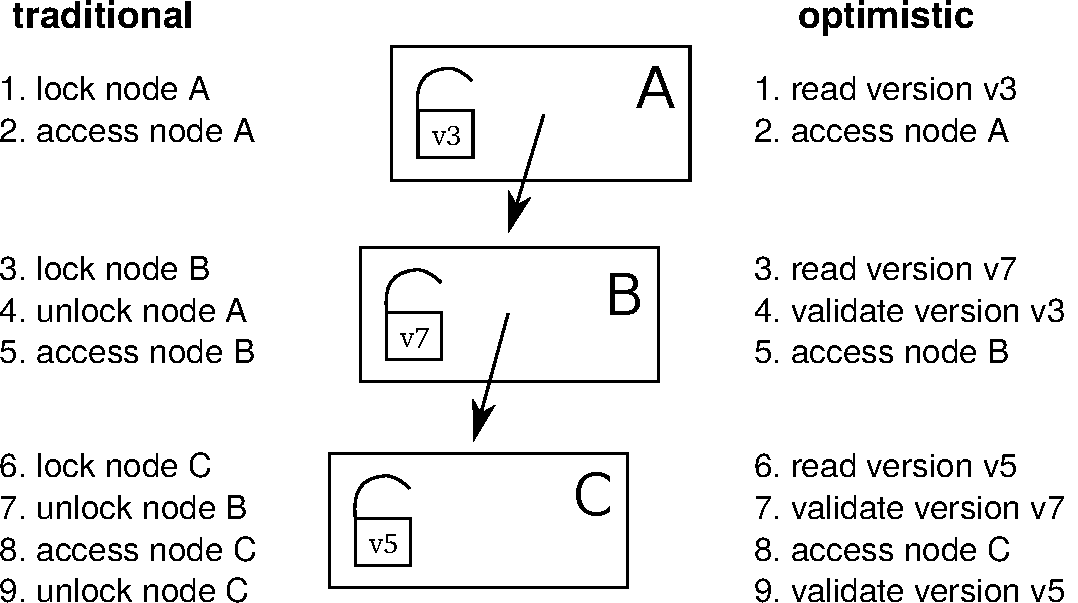
\includegraphics[width=0.65\linewidth]{olcall.pdf}
  \vspace{0.2cm}
  \caption{Comparison of a lookup operation in a 3-level tree using traditional lock coupling (left-hand side) vs.~optimistic lock coupling (right-hand side).}
  \label{fig:olc}
\end{figure}

The traditional and most common lock-based synchronization protocol for B-trees is lock coupling, which interleaves lock acquisitions while holding at most two locks at a time.
If, as we observed earlier, optimistic locks have similar semantics as traditional locks, it is natural to ask whether lock coupling can be combined with optimistic locks.
And indeed the answer is yes: One can almost mechanically translate traditional lock coupling code to optimistic lock coupling code.
This is illustrated in Figure~\ref{fig:olc}, which compares the traversal in a tree of height 3 using traditional and optimistic locks.
As the figure shows, the main difference is that locking is translated to reading the version and that unlocking becomes validation of the previously read version.
This simple change provides efficient lock-free tree traversal without the need to design a complex synchronization protocol.

It is important to emphasize the conceptual simplicity of OLC in comparison to data structures that use custom protocols like the Bw-tree~\cite{DBLP:conf/icde/LevandoskiLS13a}.
To implement lock-free access, the Bw-tree requires an indirection table, delta nodes, complex splitting and merging logic, retry logic, etc.
OLC, on the other hand, can directly be applied to B-trees mostly by adding the appropriate optimistic locking code and without modifying the node layout itself.
Therefore, OpenBw-Tree, an open source implementation of the Bw-tree, requires an order of magnitude more code than a B-tree based on OLC\footnote{Both implementations are available on GitHub: \url{https://github.com/wangziqi2016/index-microbench}}.
Given how difficult it is to develop, validate, and debug lock-free code, simplicity is obviously a major advantage.

\subsection{Correctness Aspects}

\begin{figure}
  % \centering
  %[basicstyle=\normalsize\ttfamily,showstringspaces=false,columns=fullflexible,breaklines=false,breakatwhitespace=true,numbers=none,numberstyle=\small,style=C,keepspaces=true]
\begin{lstlisting}[basicstyle=\ttfamily,language=C++,numbers=left,numberstyle=\small]
std::atomic<BTreeNode*> root;

// search for key in B+tree, returns payload in resultOut
bool lookup(Key key, Value& resultOut) {
   BTreeNode* node = root.load();
   uint64_t nodeVersion = node->readLockOrRestart();
   if (node != root.load()) // make sure the root is still the root
      restart();

   BTreeInner<Key>* parent = nullptr;
   uint64_t parentVersion = 0;

   while (node->isInner()) {
      auto inner = (BTreeInner*)node;

      // unlock parent and make current node the parent
      if (parent)
         parent->readUnlockOrRestart(parentVersion);
      parent = inner;
      parentVersion = nodeVersion;

      // search for next node
      node = inner->findChild(key);
      // validate 'inner' to ensure that 'node' pointer is valid
      inner->checkOrRestart(nodeVersion);
      // now it safe to dereference 'node' pointer (read its version)
      nodeVersion = node->readLockOrRestart();
   }

   // search in leaf and retrieve payload
   auto leaf = (BTreeLeaf*)node;
   bool success = leaf->findValue(key, resultOut);

   // unlock everything
   if (parent)
      parent->readUnlockOrRestart(parentVersion);
   node->readUnlockOrRestart(nodeVersion);

   return success;
}
\end{lstlisting}
  \vspace{0.2cm}
  \caption{B-tree lookup code using OLC. For simplicity, the restart logic is not shown.}
  \label{fig:lookup}
\end{figure}

So far, we have introduced the high-level ideas behind OLC and have stressed its similarity to traditional lock coupling.
Let us now discuss some cases where the close similarity between lock coupling and OLC breaks down.
To make this more concrete, we show the B-tree lookup code in Figure~\ref{fig:lookup}.
In the code, \texttt{readLockOrRestart} reads the lock version and \texttt{readUnlockOrRestart} validates that the read was correct.

One issue with OLC is that any pointer speculatively read from a node may point to invalid memory (if that node is modified concurrently).
Dereferencing such a pointer (e.g., to read its optimistic lock), may cause a segmentation fault or undefined behavior.
In the code shown in Figure~\ref{fig:lookup}, this problem is prevented by the extra check in line 25, which ensures that the read from the node containing the pointer was correct.
Without this additional validation, the code would in line 27 dereference the pointer speculatively read in line 23.
Note that the implementation of \texttt{checkOrRestart} is actually identical to \texttt{readUnlockOrRestart}.
We chose to give it a different name to highlight the fact that this extra check would not be necessary with read/write locks.

Another potential issue with optimistic locks is code that does not terminate.
Code that speculatively accesses a node, like an intra-node binary search, should be written in a way such that it always terminates---even in the presence of concurrent writes.
Otherwise, the validation code that detects the concurrent write will never run.
The binary search of a B-tree, for example, needs to be written in such a way that each comparison makes progress.
For some data structures that do not require loops in the traversal code (like ART) termination is trivially true.

\subsection{Implementation Details}

% implementation, efficiency
To implement an optimistic lock, one can combine the lock and the version counter into a single 64-bit\footnote{Even after subtracting one bit for the lock status, a back-of-the-envelope calculation can show that 63 bits are large enough to never overflow in practice.} word~\cite{artsync}.
A typical read operation will therefore merely consist of reading this version counter atomically.
In C++11 this can be implemented using the \texttt{std::atomic} type.

On x86, atomic reads are cheap because of x86's strong memory order guarantees.
No memory fences are required for sequentially-consistent loads, which are translated (by both GCC and clang) into standard \texttt{MOV} instructions.
Hence, the only effect of \texttt{std::atomic} for loads is preventing instruction re-ordering.
This makes version access and validation cheap.
Acquiring and releasing an optimistic lock in exclusive mode has comparable cost to a traditional lock:
A fairly expensive sequentially-consistent store is needed for acquiring a lock, while a standard \texttt{MOV} suffices for releasing it.
A simple sinlock-based implementation of optimistic locks can be found in the appendix of an earlier paper~\cite{artsync}.

OLC code must be able to handle restarts since validation or lock upgrade can fail due to concurrent writers.
Restarts can easily be implemented by wrapping the data structure operation in a loop (for simplicity not shown in Figure~\ref{fig:lookup}).
Such a loop also enables limiting the number of optimistic retry operations and falling back to pessimistic locking in cases of very heavy contention.
The ability to fall back to traditional locking is a major advantage of OLC in terms of robustness over lock-free approaches, which do not have this option.

In addition to the optimistic shared mode and the exclusive mode, optimistic locks also support a ``shared pessimistic'' mode, which physically acquires the lock in shared mode (allowing multiple concurrent readers but no writers).
This mode is useful for table (or range) scans that touch many tuples on a leaf page (which would otherwise easily abort).
Finally, let us mention that large range scans and table scans, should be broken up into several per-node traversals as is done in the LeanStore~\cite{leanstore} system.

Like all lock-free data structures, but unlike traditional locking and Hardware Transactional Memory~\cite{DBLP:conf/hpca/KarnagelDRLLSL14,DBLP:journals/pvldb/MakreshanskiLS15,htmtkde}, OLC requires care when deleting (and reusing) nodes.
The reason is that a deleting thread can never be sure that a node can be reclaimed because other threads might still be optimistically reading from that node.
Therefore, standard solutions like epoch-based reclamation~\cite{DBLP:conf/sosp/TuZKLM13}, hazard pointers~\cite{DBLP:journals/tpds/Michael04}, or optimized hazard pointers~\cite{DBLP:conf/spaa/BalmauGHZ16} need to be used.
These memory reclamation techniques are, however, largely orthogonal to the synchronization protocol itself.

%-lock-free is not a strong guarantee

\newpage
\section{Evaluation}\label{sec:evaluation}

Let us now experimentally evaluate the overhead and scalability of OLC.
For the experiments, we use an in-memory B+tree implemented in C++11 using templates, which is configured to use nodes of 4096 bytes, random 8 byte keys, and 8 byte payloads.
Based on this B-tree, we compare the following synchronization approaches:
\begin{itemize}
\item an OLC implementation\footnote{An almost identical OLC implementation is available on github: \url{https://github.com/wangziqi2016/index-microbench/tree/master/BTreeOLC}}
\item a variant based on traditional lock coupling and read/write locks
\item the unsynchronized B-tree, which obviously is only correct for read-only workloads but allows measuring the overhead of synchronization
\end{itemize}
Note that earlier work has compared the OLC implementation with a Bw-tree implementation~\cite{buzzword} and other state-of-the-art in-memory index structures.

We use a Haswell EP system with an Intel Xeon E5-2687W v3 CPU, which has 10 cores (20 ``Hyper-Threads'') and 25~MB of L3 cache.
The system is running Ubuntu 18.10 and we use GCC 8.2.0 to compile our code.
The CPU counters are obtained using the Linux perf API\footnote{We use the following convenience wrapper: \url{https://github.com/viktorleis/perfevent}}.

\begin{table}
  \caption{Performance and CPU counters for lookup and insert operations in a B-tree with 100M keys. We perform 100M operations and normalize the CPU counters by that number.}
  \label{tab:overhead}
  \centering
  \begin{tabular}{lrrrrrrr}\toprule
                    &         &        &        & instruc-  & L1     & L3     & branch \\
                    & threads & M op/s & cycles & tions & misses & misses & misses \\\midrule
lookup (no sync.)   & 1       & 1.72   & 2028   & 283     & 39.1   & 14.9   & 16.1   \\
lookup (OLC)        & 1       & 1.65   & 2107   & 370     & 43.9   & 15.1   & 16.7   \\
lookup (lock coup.) & 1       & 1.72   & 2078   & 365     & 42.3   & 16.9   & 15.7   \\\midrule
insert (no sync.)   & 1       & 1.51   & 2286   & 530     & 59.8   & 31.1   & 17.3   \\
insert (OLC)        & 1       & 1.50   & 2303   & 629     & 61.2   & 31.1   & 16.5   \\
insert (lock coup.) & 1       & 1.41   & 2473   & 644     & 61.0   & 31.0   & 17.2   \\\midrule
lookup (no sync.)   & 10      & 15.48  & 2058   & 283     & 38.6   & 15.5   & 16.0   \\
lookup (OLC)        & 10      & 14.60  & 2187   & 370     & 43.8   & 15.8   & 16.8   \\
lookup (lock coup.) & 10      & 5.71   & 5591   & 379     & 54.2   & 17.0   & 14.8   \\\midrule
insert (no sync.)   & 10      & -      & -      & -       & -      & -      & -      \\
insert (OLC)        & 10      & 10.46  & 2940   & 656     & 62.0   & 32.5   & 16.8   \\
insert (lock coup.) & 10      & 7.55   & 4161   & 667     & 75.0   & 28.6   & 16.2   \\
    \bottomrule
\end{tabular}
\end{table}

Table~\ref{tab:overhead} compares the performance and CPU counters for lookup and insert operations in a B-tree with 100M keys.
With {\em single-threaded} execution, we observe that all three approaches have very similar performance.
Adding traditional or optimistic locks to unsynchronized B-tree code results in up to 30\% of additional instructions without affecting single-threaded performance much.

\begin{figure}
  \centering
  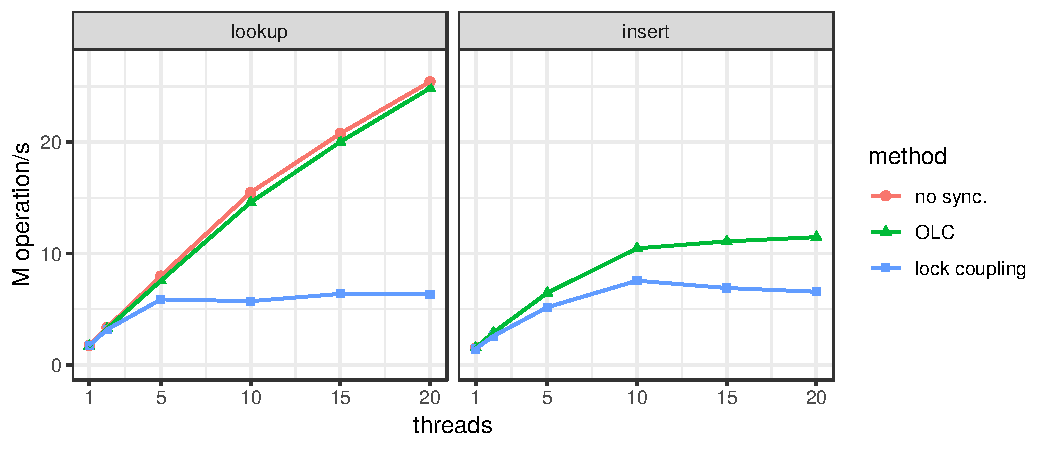
\includegraphics[width=\linewidth]{scale.pdf}
  \vspace{0.2cm}
  \caption{Scalability on 10-core system for B-tree operations (100M values).}
  \label{fig:scale}
\end{figure}

As Figure~\ref{fig:scale} shows, the results change dramatically once we use multiple threads.
For lookup, the scalability of OLC is near-linear up to 20 threads, even though the system has only 10 ``real cores''.
The OLC scalability for insert is also respectable (though not quite as linear because multi-threaded insertion approaches the memory bandwidth of our processor).
The figure also shows that the results of traditional lock coupling with read/write locks are significantly worse than OLC.
With 20 threads, lookup with OLC is 3.9$\times$ faster than traditional lock coupling.

\section{Summary}\label{sec:conc}

Optimistic Lock Coupling (OLC) is an effective synchronization method that combines the simplicity of traditional lock coupling with the superior scalability of lock-free approaches.
OLC is widely applicable and has already been successfully used to synchronize several data structures, including B-trees, binary search trees, and different trie variants.
These features make it highly attractive for modern database systems as well as performance-critical systems software in general.

\begin{thebibliography}{10}

\bibitem{DBLP:conf/spaa/BalmauGHZ16}
O.~Balmau, R.~Guerraoui, M.~Herlihy, and I.~Zablotchi.
\newblock Fast and robust memory reclamation for concurrent data structures.
\newblock In {\em SPAA}, 2016.

\bibitem{DBLP:journals/acta/BayerS77}
R.~Bayer and M.~Schkolnick.
\newblock Concurrency of operations on {B}-trees.
\newblock {\em Acta Informatica}, 9, 1977.

\bibitem{hot}
R.~Binna, E.~Zangerle, M.~Pichl, G.~Specht, and V.~Leis.
\newblock {HOT}: A height optimized trie index for main-memory database
  systems.
\newblock In {\em SIGMOD}, 2018.

\bibitem{DBLP:conf/ppopp/BronsonCCO10}
N.~G. Bronson, J.~Casper, H.~Chafi, and K.~Olukotun.
\newblock A practical concurrent binary search tree.
\newblock In {\em PPOPP}, 2010.

\bibitem{DBLP:conf/vldb/ChaHKK01}
S.~K. Cha, S.~Hwang, K.~Kim, and K.~Kwon.
\newblock Cache-conscious concurrency control of main-memory indexes on
  shared-memory multiprocessor systems.
\newblock In {\em VLDB}, 2001.

\bibitem{intel}
I.~Cutress.
\newblock {Intel} goes for 48-cores: {Cascade-AP} with multi-chip package
  coming soon.
\newblock
  \url{https://www.anandtech.com/show/13535/intel-goes-for-48cores-cascade-ap},
  2018 (accessed January, 2019).

\bibitem{DBLP:conf/cidr/FaleiroA17}
J.~M. Faleiro and D.~J. Abadi.
\newblock Latch-free synchronization in database systems: Silver bullet or
  fool's gold?
\newblock In {\em CIDR}, 2017.

\bibitem{DBLP:journals/ftdb/Graefe11}
G.~Graefe.
\newblock Modern {B}-tree techniques.
\newblock {\em Foundations and Trends in Databases}, 3(4), 2011.

\bibitem{DBLP:conf/hpca/KarnagelDRLLSL14}
T.~Karnagel, R.~Dementiev, R.~Rajwar, K.~Lai, T.~Legler, B.~Schlegel, and
  W.~Lehner.
\newblock Improving in-memory database index performance with
  {Intel}\({}^{\mbox{{\textregistered}}}\) transactional synchronization
  extensions.
\newblock In {\em HPCA}, 2014.

\bibitem{DBLP:journals/tods/LehmanY81}
P.~L. Lehman and S.~B. Yao.
\newblock Efficient locking for concurrent operations on {B}-trees.
\newblock {\em {ACM} Trans. Database Syst.}, 6(4), 1981.

\bibitem{leanstore}
V.~Leis, M.~Haubenschild, A.~Kemper, and T.~Neumann.
\newblock Leanstore: In-memory data management beyond main memory.
\newblock In {\em ICDE}, 2018.

\bibitem{art}
V.~Leis, A.~Kemper, and T.~Neumann.
\newblock The adaptive radix tree: {ARTful} indexing for main-memory databases.
\newblock In {\em ICDE}, 2013.

\bibitem{htmtkde}
V.~Leis, A.~Kemper, and T.~Neumann.
\newblock Scaling {HTM}-supported database transactions to many cores.
\newblock {\em {IEEE} Trans. Knowl. Data Eng.}, 28(2), 2016.

\bibitem{artsync}
V.~Leis, F.~Scheibner, A.~Kemper, and T.~Neumann.
\newblock The {ART} of practical synchronization.
\newblock In {\em DaMoN}, 2016.

\bibitem{DBLP:conf/icde/LevandoskiLS13a}
J.~J. Levandoski, D.~B. Lomet, and S.~Sengupta.
\newblock The {Bw}-tree: A {B}-tree for new hardware platforms.
\newblock In {\em ICDE}, 2013.

\bibitem{DBLP:journals/pvldb/MakreshanskiLS15}
D.~Makreshanski, J.~J. Levandoski, and R.~Stutsman.
\newblock To lock, swap, or elide: On the interplay of hardware transactional
  memory and lock-free indexing.
\newblock {\em {PVLDB}}, 8(11), 2015.

\bibitem{DBLP:dblp_conf/eurosys/MaoKM12}
Y.~Mao, E.~Kohler, and R.~T. Morris.
\newblock Cache craftiness for fast multicore key-value storage.
\newblock In {\em EuroSys}, 2012.

\bibitem{DBLP:journals/tpds/Michael04}
M.~M. Michael.
\newblock Hazard pointers: Safe memory reclamation for lock-free objects.
\newblock {\em {IEEE} Trans. Parallel Distrib. Syst.}, 15(6), 2004.

\bibitem{DBLP:journals/jacm/ShalevS06}
O.~Shalev and N.~Shavit.
\newblock Split-ordered lists: Lock-free extensible hash tables.
\newblock {\em J. {ACM}}, 53(3), 2006.

\bibitem{amd}
A.~Shilov.
\newblock {AMD} previews {EPYC} ‘{Rome}’ processor: Up to 64 {Zen} 2 cores.
\newblock
  \url{https://www.anandtech.com/show/13561/amd-previews-epyc-rome-processor-up-to-64-zen-2-cores},
  2018 (accessed January, 2019).

\bibitem{DBLP:conf/sosp/TuZKLM13}
S.~Tu, W.~Zheng, E.~Kohler, B.~Liskov, and S.~Madden.
\newblock Speedy transactions in multicore in-memory databases.
\newblock In {\em SOSP}, 2013.

\bibitem{buzzword}
Z.~Wang, A.~Pavlo, H.~Lim, V.~Leis, H.~Zhang, M.~Kaminsky, and D.~Andersen.
\newblock Building a {Bw}-tree takes more than just buzz words.
\newblock In {\em SIGMOD}, 2018.

\end{thebibliography}


%\bibliographystyle{abbrv}
%\bibliography{main}

\end{document}

\end{article}

\begin{article}
{Responsible AI Challenges in End-to-end Machine Learning}
{Steven Euijong Whang, Ki Hyun Tae, Yuji Roh and Geon Heo}
\pdfminorversion=5
\documentclass[11pt]{article}
\usepackage{deauthor,times,graphicx,caption,microtype}
\usepackage{hyperref}
\usepackage{listings}
\usepackage{booktabs}

\begin{document}

\title{Optimistic Lock Coupling: A Scalable and Efficient General-Purpose Synchronization Method}

\author{Viktor Leis, Michael Haubenschild\raisebox{0.9ex}{$\ast$}, Thomas Neumann\\ Technische Universit{\"a}t M{\"u}nchen \hspace{0.7cm} Tableau Software\raisebox{0.9ex}{$\ast$} \\ {\{leis,neumann\}{@}in.tum.de} \hspace{0.7cm} {mhaubenschild{@}tableau.com\raisebox{0.9ex}{$\ast$}}}

\maketitle

\begin{abstract}
As the number of cores on commodity processors continues to increase, scalability becomes more and more crucial for overall performance.
Scalable and efficient concurrent data structures are particularly important, as these are often the building blocks of parallel algorithms.
Unfortunately, traditional synchronization techniques based on fine-grained locking have been shown to be unscalable on modern multi-core CPUs.
Lock-free data structures, on the other hand, are extremely difficult to design and often incur significant overhead.

In this work, we make the case for Optimistic Lock Coupling as a practical alternative to both traditional locking and the lock-free approach.
We show that Optimistic Lock Coupling is highly scalable and almost as simple to implement as traditional lock coupling.
Another important advantage is that it is easily applicable to most tree-like data structures.
We therefore argue that Optimistic Lock Coupling, rather than a complex and error-prone custom synchronization protocol, should be the default choice for performance-critical data structures.
\end{abstract}

\section{Introduction}

% more and more cores
Today, Intel's commodity server processors have up to 28 cores and its upcoming microarchitecture will have up to 48 cores per socket~\cite{intel}.
Similarly, AMD currently stands at 32 cores and this number is expected to double in the next generation~\cite{amd}.
Since both platforms support simultaneous multithreading (also known as hyperthreading), affordable commodity servers (with up to two sockets) will soon routinely have between 100 and 200 hardware threads.

% data structure scalability is important
With such a high degree of hardware parallelism, efficient data processing crucially depends on how well concurrent data structures scale.
Internally, database systems use a plethora of data structures like table heaps, internal work queues, and, most importantly, index structures.
Any of these can easily become a scalability (and therefore overall performance) bottleneck on many-core CPUs.

% traditional synchronization: fine-grained locks, slow, cache invalidation
Traditionally, database systems synchronize internal data structures using fine-grained reader/writer locks\footnote{In this work, we focus on data structure synchronization rather than high-level transaction semantics and therefore use the term {\em lock} for what would typically be called {\em latch} in the database literature. We thus follow common computer science (rather than database) terminology.}.
Unfortunately, while fine-grained locking makes lock contention unlikely, it still results in bad scalability because lock acquisition and release require writing to shared memory.
Due to the way cache coherency is implemented on modern multi-core CPUs, these writes cause additional cache misses\footnote{The cache coherency protocol ensures that all copies of a cache line on other cores are invalidated before the write can proceed.} and the cache line containing the lock's internal data becomes a point of physical contention.
As a result, any frequently-accessed lock (e.g., the lock of the root node of a B-tree) severely limits scalability.

% lock-free bw-tree: no more latches, but indirections, extremely complex
Lock-free data structures like the Bw-tree~\cite{DBLP:conf/icde/LevandoskiLS13a} (a lock-free B-tree variant) or the Split-Ordered List~\cite{DBLP:journals/jacm/ShalevS06} (a lock-free hash table) do not acquire any locks and therefore generally scale much better than locking-based approaches (in particular for read-mostly workloads).
However, lock-free synchronization has other downsides:
First, it is very difficult and results in extremely complex and error-prone code (when compared to locking).
Second, because the functionality of atomic primitives provided by the hardware (e.g., atomically compare-and-swap 8 bytes) is limited, complex operations require additional indirections within the data structure.
For example, the Bw-tree requires an indirection table and the Split-Ordered List requires ``dummy nodes'', resulting in overhead due to additional cache misses.

% OLC for the win
In this paper we make the case for {\em Optimistic Lock Coupling (OLC)}, a synchronization method that combines some of the best properties of lock-based and lock-free synchronization.
OLC utilizes a special lock type that can be used in two modes:
The first mode is similar to a traditional mutex and excludes other threads by physically acquiring the underlying lock.
In the second mode, reads can proceed optimistically by validating a version counter that is embedded in the lock (similar to optimistic concurrency control).
The first mode is typically used by writers and the second mode by readers.
Besides this special lock type, OLC is based on the observation that optimistic lock validations can be interleaved/coupled---similar to the pair-wise interleaved lock acquisition of traditional lock coupling.
Hence, the name Optimistic Lock Coupling.

OLC has a number of desirable features:
\begin{itemize}
\item By reducing the number of writes to shared memory locations and thereby avoiding cache invalidations, it {\bf scales well} for most workloads.
\item In comparison to unsynchronized code, it requires few additional CPU instructions making it {\bf efficient}.
\item OLC is {\bf widely applicable} to different data structures. It has already been successfully used for synchronizing binary search trees~\cite{DBLP:conf/ppopp/BronsonCCO10}, tries~\cite{artsync}, trie/B-tree hybrids~\cite{DBLP:dblp_conf/eurosys/MaoKM12}, and B-trees~\cite{buzzword}.
\item In comparison to the lock-free paradigm, it is also {\bf easy to use} and requires few modifications to existing, single-threaded data structures.
\end{itemize}
Despite these positive features and its simplicity, OLC is not yet widely known.
The goal of this paper is therefore to popularize this simple idea and to make a case for it.
We argue that OLC deserves to be widely known.
It is a good default synchronization paradigm---more complex, data structure-specific protocols are seldom beneficial.

The rest of the paper is organized as follows.
Section~\ref{sec:related} discusses related work, tracing the history of OLC and its underlying ideas in the literature.
The core of the paper is Section~\ref{sec:olc}, which describes the ideas behind OLC and how it can be used to synchronize complex data structures.
In Section~\ref{sec:evaluation} we experimentally show that OLC has low overhead and scales well when used to synchronize an in-memory B-tree.
We summarize the paper in Section~\ref{sec:conc}.

\newpage
\section{Related Work}\label{sec:related}

Lock coupling has been proposed as a method for allowing concurrent operations on B-trees in 1977~\cite{DBLP:journals/acta/BayerS77}.
This traditional and still widely-used method, described in detail in Graefe's B-tree survey~\cite{DBLP:journals/ftdb/Graefe11}, is also called ``latch coupling'', ``hand-over-hand locking'', and ``crabbing''.
Because at most two locks are held at-a-time during tree traversal, this technique seemingly allows for a high degree of parallelism---in particular if read/write locks are used to enable inner nodes to be locked in shared mode.
However, as we show in Section~\ref{sec:evaluation}, on modern hardware lock acquisition (even in shared mode) results in suboptimal scalability.

An early alternative from 1981 is a B-tree variant called B-link tree~\cite{DBLP:journals/tods/LehmanY81}, which only holds a single lock at a time.
It is based on the observation that between the release of the parent lock and the acquisition of the child lock, the only ``dangerous'' thing that could have happened is the split of a child node (assuming one does not implement merge operations).
Thus, when a split happens, the key being searched might end up on a neighboring node to the right of the current child node.
A B-link tree traversal therefore detects this condition and, if needed, transparently proceeds to the neighboring node.
Releasing the parent lock early is highly beneficial when the child node needs to be fetched from disk.
For in-memory workloads, however, the B-link tree has the same scalability issues as lock coupling (it acquires just as many locks).

The next major advance, Optimistic Latch-Free Index Traversal (OLFIT)~\cite{DBLP:conf/vldb/ChaHKK01}, was proposed in 2001.
OLFIT introduced the idea of a combined lock/update counter, which we call {\em optimistic lock}. % , for lack of a better name,
Based on these per-node optimistic locks and the synchronization protocol of the B-link tree, OLFIT finally achieves good scalability on parallel processors.
The OLFIT protocol is fairly complex, as it requires both the non-trivial B-link protocol and optimistic locks.
Furthermore, like the B-link tree protocol, it does not support merging nodes, and is specific to B-trees (cannot easily be applied to other data structures).

In the following two decades, the growth of main-memory capacity led to much research into other data structures besides the venerable B-tree.
Particularly relevant for our discussion is Bronson et al.'s~\cite{DBLP:conf/ppopp/BronsonCCO10} concurrent binary search tree, which is based on optimistic version validation and has a sophisticated, data structure-specific synchronization protocol.
To the best of our knowledge, this 2010 paper is the first that, as part of its protocol, interleaves version validation across nodes---rather than validating each node separately like OLFIT.
In that paper, this idea is called ``hand-over-hand, optimistic validation'', while we prefer the term Optimistic Lock Coupling to highlight the close resemblance to traditional lock coupling.
Similarly, Mao et al.'s~\cite{DBLP:dblp_conf/eurosys/MaoKM12} Masstree (a concurrent hybrid trie/B-tree) is also based on the same ideas, but again uses them as part of a more complex protocol.

The Adaptive Radix Tree (ART)~\cite{art} is another recent in-memory data structure, which we proposed in 2013.
In contrast to the two data structures just mentioned, it was originally designed with single-threaded performance in mind without supporting concurrency.
To add support for concurrency, we initially started designing a custom protocol called Read-Optimized Write Exclusion (ROWEX)~\cite{artsync}, which turned out to be non-trivial and requires modifications of the underlying data structure\footnote{Note that ROWEX is already easier to apply to existing data structures than the lock-free approach. The difficulty depends on the data structure. Applying ROWEX is hard for B-trees with sorted keys and fairly easy for copy-on-write data structures like the Height Optimized Trie~\cite{hot}---with ART being somewhere in the middle.}.
However, fairly late in the project, we also realized, that OLC {\em alone} (rather than as part of a more complex protocol) is sufficient to synchronize ART.
No other changes to the data structure were necessary.
Both approaches were published and experimentally evaluated in a followup paper~\cite{artsync}, which shows that, despite its simplicity, OLC is efficient, scalable, and generally outperforms ROWEX.

Similar results were recently published regarding B-trees~\cite{buzzword}.
In this experimental study a simple OLC-based synchronization outperformed the Bw-tree~\cite{DBLP:conf/icde/LevandoskiLS13a}, a complex lock-free synchronization approach.
Another recent paper shows that for write-intensive workloads, locking often performs better than lock-free synchronization~\cite{DBLP:conf/cidr/FaleiroA17}.
These experiences indicate that OLC is a general-purpose synchronization paradigm and motivate the current paper.

%foster b-tree\cite{DBLP:journals/tods/GraefeKK12}
%Shasha theory~\cite{DBLP:journals/tods/ShashaG88}

\section{Optimistic Lock Coupling}\label{sec:olc}

% locks suck
The standard technique for inter-thread synchronization is mutual exclusion using fine-grained locks.
In a B-tree, for example, every node usually has its own associated lock, which is acquired before accessing that node.
The problem of locking on modern multi- and many-core processors is that lock acquisition and release require writing to the shared memory location that implements the lock.
This write causes exclusive ownership of the underlying cache line and invalidates copies of it on all other processor cores.
For hierarchical, tree-like data structures, the lock of the root node becomes a point of physical contention---even in read-only workloads and even when read/write locks are used.
Depending on the specific data structure, number of cores, cache coherency protocol implementation, cache topology, whether Non-Uniform Memory Access (NUMA) is used, locking can even result in multi-threaded performance that is worse than single-threaded execution.

% in b-trees this happens very much
The inherent pessimism of locking is particularly unfortunate for B-trees:
Despite the fact that logical modifications of the root node are very infrequent, every B-tree operation must lock the root node during tree traversal\footnote{To a lesser extent this obviously applies to all inner nodes, not just the root.}.
Even the vast majority of update operations (with the exception of splits and merges), only modify a single leaf node.
These observations indicate that a more optimistic approach, which does not require locking inner nodes, would be very beneficial for B-trees.

\subsection{Optimistic Locks}

% optimism to the rescue
As the name indicates, optimistic locks try to solve the scalability issues of traditional locks using an optimistic approach.
Instead of always physically acquiring locks, even for nodes that are unlikely to be modified simultaneously, after-the-fact validation is used to detect conflicts.
This is done by augmenting each lock with a version/update counter that is incremented on every modification.
Using this version counter, readers can optimistically proceed before validating that the version did not change to ensure that the read was safe.
If validation fails, the operation is restarted.

% details on opt locks
Using optimistic locks, a read-only node access (i.e., the majority of all operations in a B-tree) does not acquire the lock and does not increment the version counter.
Instead, it performs the following steps:
\begin{enumerate}
\item read lock version (restart if lock is not free)
\item access node
\item read the version again and validate that it has not changed in the meantime
\end{enumerate}
If the last step (the validation) fails, the operation has to be restarted.
Write operations, on the other hand, are more similar to traditional locking:
\begin{enumerate}
\item acquire lock (wait if necessary)
\item access/write to node
\item increment version and unlock node
\end{enumerate}
Writes can therefore protect a node from other writes.

% similar to locks
As we observed in an earlier paper~\cite{artsync}, because of similar semantics, optimistic locks can be hidden behind an API very similar to traditional read/write locks.
Both approaches have an exclusive lock mode, and acquiring a traditional lock in shared mode is analogous to optimistic version validation.
Furthermore, like with some implementations of traditional read/write locks, optimistic locks allow upgrading a shared lock to an exclusive lock.
Lock upgrades are, for example, used to avoid most B-tree update operations from having to lock inner nodes.
In our experience, the close resemblance of optimistic and traditional locks simplifies the reasoning about optimistic locks;
one can apply similar thinking as in traditional lock-based protocols.

\subsection{Lock Coupling with Optimistic Locks}

\begin{figure}
  \centering
  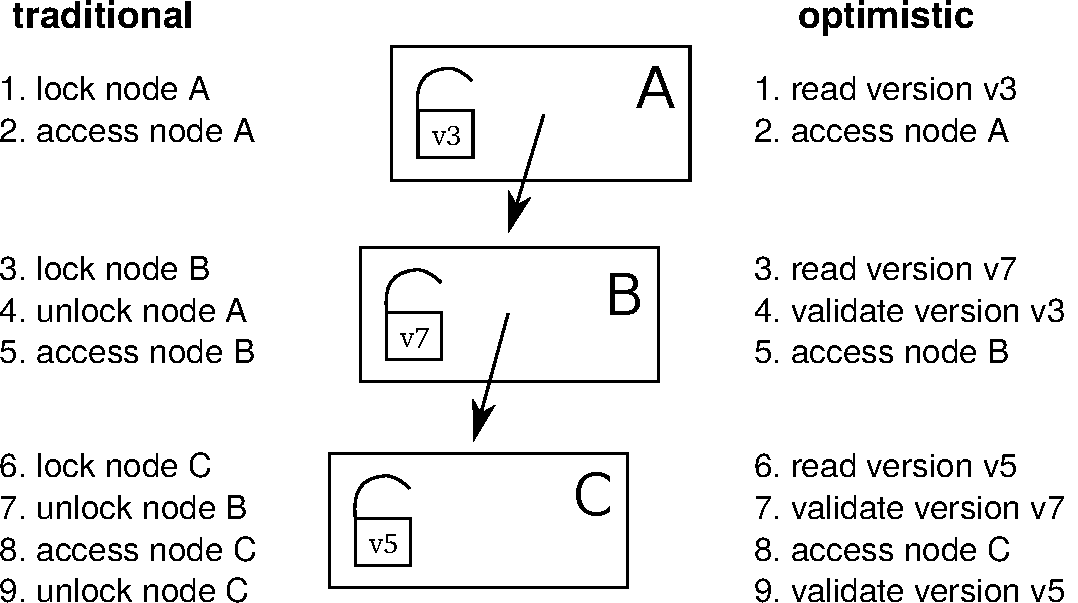
\includegraphics[width=0.65\linewidth]{olcall.pdf}
  \vspace{0.2cm}
  \caption{Comparison of a lookup operation in a 3-level tree using traditional lock coupling (left-hand side) vs.~optimistic lock coupling (right-hand side).}
  \label{fig:olc}
\end{figure}

The traditional and most common lock-based synchronization protocol for B-trees is lock coupling, which interleaves lock acquisitions while holding at most two locks at a time.
If, as we observed earlier, optimistic locks have similar semantics as traditional locks, it is natural to ask whether lock coupling can be combined with optimistic locks.
And indeed the answer is yes: One can almost mechanically translate traditional lock coupling code to optimistic lock coupling code.
This is illustrated in Figure~\ref{fig:olc}, which compares the traversal in a tree of height 3 using traditional and optimistic locks.
As the figure shows, the main difference is that locking is translated to reading the version and that unlocking becomes validation of the previously read version.
This simple change provides efficient lock-free tree traversal without the need to design a complex synchronization protocol.

It is important to emphasize the conceptual simplicity of OLC in comparison to data structures that use custom protocols like the Bw-tree~\cite{DBLP:conf/icde/LevandoskiLS13a}.
To implement lock-free access, the Bw-tree requires an indirection table, delta nodes, complex splitting and merging logic, retry logic, etc.
OLC, on the other hand, can directly be applied to B-trees mostly by adding the appropriate optimistic locking code and without modifying the node layout itself.
Therefore, OpenBw-Tree, an open source implementation of the Bw-tree, requires an order of magnitude more code than a B-tree based on OLC\footnote{Both implementations are available on GitHub: \url{https://github.com/wangziqi2016/index-microbench}}.
Given how difficult it is to develop, validate, and debug lock-free code, simplicity is obviously a major advantage.

\subsection{Correctness Aspects}

\begin{figure}
  % \centering
  %[basicstyle=\normalsize\ttfamily,showstringspaces=false,columns=fullflexible,breaklines=false,breakatwhitespace=true,numbers=none,numberstyle=\small,style=C,keepspaces=true]
\begin{lstlisting}[basicstyle=\ttfamily,language=C++,numbers=left,numberstyle=\small]
std::atomic<BTreeNode*> root;

// search for key in B+tree, returns payload in resultOut
bool lookup(Key key, Value& resultOut) {
   BTreeNode* node = root.load();
   uint64_t nodeVersion = node->readLockOrRestart();
   if (node != root.load()) // make sure the root is still the root
      restart();

   BTreeInner<Key>* parent = nullptr;
   uint64_t parentVersion = 0;

   while (node->isInner()) {
      auto inner = (BTreeInner*)node;

      // unlock parent and make current node the parent
      if (parent)
         parent->readUnlockOrRestart(parentVersion);
      parent = inner;
      parentVersion = nodeVersion;

      // search for next node
      node = inner->findChild(key);
      // validate 'inner' to ensure that 'node' pointer is valid
      inner->checkOrRestart(nodeVersion);
      // now it safe to dereference 'node' pointer (read its version)
      nodeVersion = node->readLockOrRestart();
   }

   // search in leaf and retrieve payload
   auto leaf = (BTreeLeaf*)node;
   bool success = leaf->findValue(key, resultOut);

   // unlock everything
   if (parent)
      parent->readUnlockOrRestart(parentVersion);
   node->readUnlockOrRestart(nodeVersion);

   return success;
}
\end{lstlisting}
  \vspace{0.2cm}
  \caption{B-tree lookup code using OLC. For simplicity, the restart logic is not shown.}
  \label{fig:lookup}
\end{figure}

So far, we have introduced the high-level ideas behind OLC and have stressed its similarity to traditional lock coupling.
Let us now discuss some cases where the close similarity between lock coupling and OLC breaks down.
To make this more concrete, we show the B-tree lookup code in Figure~\ref{fig:lookup}.
In the code, \texttt{readLockOrRestart} reads the lock version and \texttt{readUnlockOrRestart} validates that the read was correct.

One issue with OLC is that any pointer speculatively read from a node may point to invalid memory (if that node is modified concurrently).
Dereferencing such a pointer (e.g., to read its optimistic lock), may cause a segmentation fault or undefined behavior.
In the code shown in Figure~\ref{fig:lookup}, this problem is prevented by the extra check in line 25, which ensures that the read from the node containing the pointer was correct.
Without this additional validation, the code would in line 27 dereference the pointer speculatively read in line 23.
Note that the implementation of \texttt{checkOrRestart} is actually identical to \texttt{readUnlockOrRestart}.
We chose to give it a different name to highlight the fact that this extra check would not be necessary with read/write locks.

Another potential issue with optimistic locks is code that does not terminate.
Code that speculatively accesses a node, like an intra-node binary search, should be written in a way such that it always terminates---even in the presence of concurrent writes.
Otherwise, the validation code that detects the concurrent write will never run.
The binary search of a B-tree, for example, needs to be written in such a way that each comparison makes progress.
For some data structures that do not require loops in the traversal code (like ART) termination is trivially true.

\subsection{Implementation Details}

% implementation, efficiency
To implement an optimistic lock, one can combine the lock and the version counter into a single 64-bit\footnote{Even after subtracting one bit for the lock status, a back-of-the-envelope calculation can show that 63 bits are large enough to never overflow in practice.} word~\cite{artsync}.
A typical read operation will therefore merely consist of reading this version counter atomically.
In C++11 this can be implemented using the \texttt{std::atomic} type.

On x86, atomic reads are cheap because of x86's strong memory order guarantees.
No memory fences are required for sequentially-consistent loads, which are translated (by both GCC and clang) into standard \texttt{MOV} instructions.
Hence, the only effect of \texttt{std::atomic} for loads is preventing instruction re-ordering.
This makes version access and validation cheap.
Acquiring and releasing an optimistic lock in exclusive mode has comparable cost to a traditional lock:
A fairly expensive sequentially-consistent store is needed for acquiring a lock, while a standard \texttt{MOV} suffices for releasing it.
A simple sinlock-based implementation of optimistic locks can be found in the appendix of an earlier paper~\cite{artsync}.

OLC code must be able to handle restarts since validation or lock upgrade can fail due to concurrent writers.
Restarts can easily be implemented by wrapping the data structure operation in a loop (for simplicity not shown in Figure~\ref{fig:lookup}).
Such a loop also enables limiting the number of optimistic retry operations and falling back to pessimistic locking in cases of very heavy contention.
The ability to fall back to traditional locking is a major advantage of OLC in terms of robustness over lock-free approaches, which do not have this option.

In addition to the optimistic shared mode and the exclusive mode, optimistic locks also support a ``shared pessimistic'' mode, which physically acquires the lock in shared mode (allowing multiple concurrent readers but no writers).
This mode is useful for table (or range) scans that touch many tuples on a leaf page (which would otherwise easily abort).
Finally, let us mention that large range scans and table scans, should be broken up into several per-node traversals as is done in the LeanStore~\cite{leanstore} system.

Like all lock-free data structures, but unlike traditional locking and Hardware Transactional Memory~\cite{DBLP:conf/hpca/KarnagelDRLLSL14,DBLP:journals/pvldb/MakreshanskiLS15,htmtkde}, OLC requires care when deleting (and reusing) nodes.
The reason is that a deleting thread can never be sure that a node can be reclaimed because other threads might still be optimistically reading from that node.
Therefore, standard solutions like epoch-based reclamation~\cite{DBLP:conf/sosp/TuZKLM13}, hazard pointers~\cite{DBLP:journals/tpds/Michael04}, or optimized hazard pointers~\cite{DBLP:conf/spaa/BalmauGHZ16} need to be used.
These memory reclamation techniques are, however, largely orthogonal to the synchronization protocol itself.

%-lock-free is not a strong guarantee

\newpage
\section{Evaluation}\label{sec:evaluation}

Let us now experimentally evaluate the overhead and scalability of OLC.
For the experiments, we use an in-memory B+tree implemented in C++11 using templates, which is configured to use nodes of 4096 bytes, random 8 byte keys, and 8 byte payloads.
Based on this B-tree, we compare the following synchronization approaches:
\begin{itemize}
\item an OLC implementation\footnote{An almost identical OLC implementation is available on github: \url{https://github.com/wangziqi2016/index-microbench/tree/master/BTreeOLC}}
\item a variant based on traditional lock coupling and read/write locks
\item the unsynchronized B-tree, which obviously is only correct for read-only workloads but allows measuring the overhead of synchronization
\end{itemize}
Note that earlier work has compared the OLC implementation with a Bw-tree implementation~\cite{buzzword} and other state-of-the-art in-memory index structures.

We use a Haswell EP system with an Intel Xeon E5-2687W v3 CPU, which has 10 cores (20 ``Hyper-Threads'') and 25~MB of L3 cache.
The system is running Ubuntu 18.10 and we use GCC 8.2.0 to compile our code.
The CPU counters are obtained using the Linux perf API\footnote{We use the following convenience wrapper: \url{https://github.com/viktorleis/perfevent}}.

\begin{table}
  \caption{Performance and CPU counters for lookup and insert operations in a B-tree with 100M keys. We perform 100M operations and normalize the CPU counters by that number.}
  \label{tab:overhead}
  \centering
  \begin{tabular}{lrrrrrrr}\toprule
                    &         &        &        & instruc-  & L1     & L3     & branch \\
                    & threads & M op/s & cycles & tions & misses & misses & misses \\\midrule
lookup (no sync.)   & 1       & 1.72   & 2028   & 283     & 39.1   & 14.9   & 16.1   \\
lookup (OLC)        & 1       & 1.65   & 2107   & 370     & 43.9   & 15.1   & 16.7   \\
lookup (lock coup.) & 1       & 1.72   & 2078   & 365     & 42.3   & 16.9   & 15.7   \\\midrule
insert (no sync.)   & 1       & 1.51   & 2286   & 530     & 59.8   & 31.1   & 17.3   \\
insert (OLC)        & 1       & 1.50   & 2303   & 629     & 61.2   & 31.1   & 16.5   \\
insert (lock coup.) & 1       & 1.41   & 2473   & 644     & 61.0   & 31.0   & 17.2   \\\midrule
lookup (no sync.)   & 10      & 15.48  & 2058   & 283     & 38.6   & 15.5   & 16.0   \\
lookup (OLC)        & 10      & 14.60  & 2187   & 370     & 43.8   & 15.8   & 16.8   \\
lookup (lock coup.) & 10      & 5.71   & 5591   & 379     & 54.2   & 17.0   & 14.8   \\\midrule
insert (no sync.)   & 10      & -      & -      & -       & -      & -      & -      \\
insert (OLC)        & 10      & 10.46  & 2940   & 656     & 62.0   & 32.5   & 16.8   \\
insert (lock coup.) & 10      & 7.55   & 4161   & 667     & 75.0   & 28.6   & 16.2   \\
    \bottomrule
\end{tabular}
\end{table}

Table~\ref{tab:overhead} compares the performance and CPU counters for lookup and insert operations in a B-tree with 100M keys.
With {\em single-threaded} execution, we observe that all three approaches have very similar performance.
Adding traditional or optimistic locks to unsynchronized B-tree code results in up to 30\% of additional instructions without affecting single-threaded performance much.

\begin{figure}
  \centering
  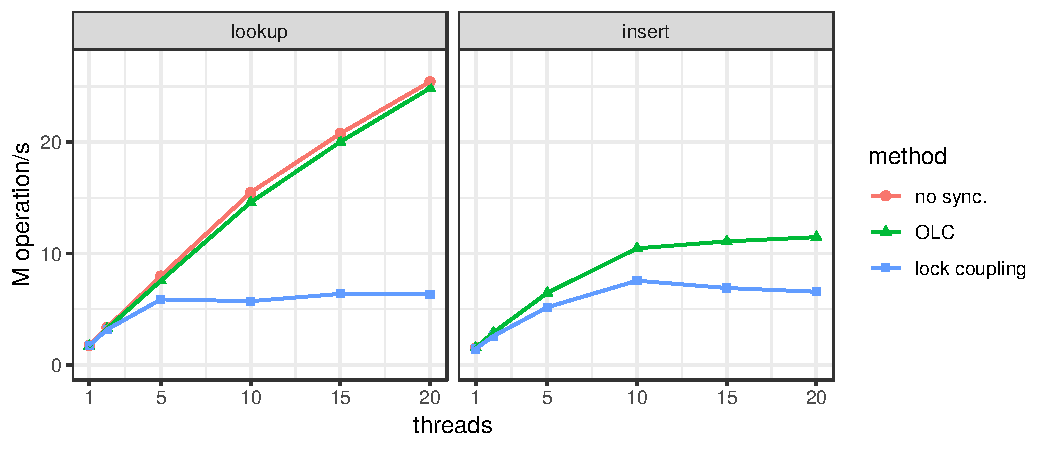
\includegraphics[width=\linewidth]{scale.pdf}
  \vspace{0.2cm}
  \caption{Scalability on 10-core system for B-tree operations (100M values).}
  \label{fig:scale}
\end{figure}

As Figure~\ref{fig:scale} shows, the results change dramatically once we use multiple threads.
For lookup, the scalability of OLC is near-linear up to 20 threads, even though the system has only 10 ``real cores''.
The OLC scalability for insert is also respectable (though not quite as linear because multi-threaded insertion approaches the memory bandwidth of our processor).
The figure also shows that the results of traditional lock coupling with read/write locks are significantly worse than OLC.
With 20 threads, lookup with OLC is 3.9$\times$ faster than traditional lock coupling.

\section{Summary}\label{sec:conc}

Optimistic Lock Coupling (OLC) is an effective synchronization method that combines the simplicity of traditional lock coupling with the superior scalability of lock-free approaches.
OLC is widely applicable and has already been successfully used to synchronize several data structures, including B-trees, binary search trees, and different trie variants.
These features make it highly attractive for modern database systems as well as performance-critical systems software in general.

\begin{thebibliography}{10}

\bibitem{DBLP:conf/spaa/BalmauGHZ16}
O.~Balmau, R.~Guerraoui, M.~Herlihy, and I.~Zablotchi.
\newblock Fast and robust memory reclamation for concurrent data structures.
\newblock In {\em SPAA}, 2016.

\bibitem{DBLP:journals/acta/BayerS77}
R.~Bayer and M.~Schkolnick.
\newblock Concurrency of operations on {B}-trees.
\newblock {\em Acta Informatica}, 9, 1977.

\bibitem{hot}
R.~Binna, E.~Zangerle, M.~Pichl, G.~Specht, and V.~Leis.
\newblock {HOT}: A height optimized trie index for main-memory database
  systems.
\newblock In {\em SIGMOD}, 2018.

\bibitem{DBLP:conf/ppopp/BronsonCCO10}
N.~G. Bronson, J.~Casper, H.~Chafi, and K.~Olukotun.
\newblock A practical concurrent binary search tree.
\newblock In {\em PPOPP}, 2010.

\bibitem{DBLP:conf/vldb/ChaHKK01}
S.~K. Cha, S.~Hwang, K.~Kim, and K.~Kwon.
\newblock Cache-conscious concurrency control of main-memory indexes on
  shared-memory multiprocessor systems.
\newblock In {\em VLDB}, 2001.

\bibitem{intel}
I.~Cutress.
\newblock {Intel} goes for 48-cores: {Cascade-AP} with multi-chip package
  coming soon.
\newblock
  \url{https://www.anandtech.com/show/13535/intel-goes-for-48cores-cascade-ap},
  2018 (accessed January, 2019).

\bibitem{DBLP:conf/cidr/FaleiroA17}
J.~M. Faleiro and D.~J. Abadi.
\newblock Latch-free synchronization in database systems: Silver bullet or
  fool's gold?
\newblock In {\em CIDR}, 2017.

\bibitem{DBLP:journals/ftdb/Graefe11}
G.~Graefe.
\newblock Modern {B}-tree techniques.
\newblock {\em Foundations and Trends in Databases}, 3(4), 2011.

\bibitem{DBLP:conf/hpca/KarnagelDRLLSL14}
T.~Karnagel, R.~Dementiev, R.~Rajwar, K.~Lai, T.~Legler, B.~Schlegel, and
  W.~Lehner.
\newblock Improving in-memory database index performance with
  {Intel}\({}^{\mbox{{\textregistered}}}\) transactional synchronization
  extensions.
\newblock In {\em HPCA}, 2014.

\bibitem{DBLP:journals/tods/LehmanY81}
P.~L. Lehman and S.~B. Yao.
\newblock Efficient locking for concurrent operations on {B}-trees.
\newblock {\em {ACM} Trans. Database Syst.}, 6(4), 1981.

\bibitem{leanstore}
V.~Leis, M.~Haubenschild, A.~Kemper, and T.~Neumann.
\newblock Leanstore: In-memory data management beyond main memory.
\newblock In {\em ICDE}, 2018.

\bibitem{art}
V.~Leis, A.~Kemper, and T.~Neumann.
\newblock The adaptive radix tree: {ARTful} indexing for main-memory databases.
\newblock In {\em ICDE}, 2013.

\bibitem{htmtkde}
V.~Leis, A.~Kemper, and T.~Neumann.
\newblock Scaling {HTM}-supported database transactions to many cores.
\newblock {\em {IEEE} Trans. Knowl. Data Eng.}, 28(2), 2016.

\bibitem{artsync}
V.~Leis, F.~Scheibner, A.~Kemper, and T.~Neumann.
\newblock The {ART} of practical synchronization.
\newblock In {\em DaMoN}, 2016.

\bibitem{DBLP:conf/icde/LevandoskiLS13a}
J.~J. Levandoski, D.~B. Lomet, and S.~Sengupta.
\newblock The {Bw}-tree: A {B}-tree for new hardware platforms.
\newblock In {\em ICDE}, 2013.

\bibitem{DBLP:journals/pvldb/MakreshanskiLS15}
D.~Makreshanski, J.~J. Levandoski, and R.~Stutsman.
\newblock To lock, swap, or elide: On the interplay of hardware transactional
  memory and lock-free indexing.
\newblock {\em {PVLDB}}, 8(11), 2015.

\bibitem{DBLP:dblp_conf/eurosys/MaoKM12}
Y.~Mao, E.~Kohler, and R.~T. Morris.
\newblock Cache craftiness for fast multicore key-value storage.
\newblock In {\em EuroSys}, 2012.

\bibitem{DBLP:journals/tpds/Michael04}
M.~M. Michael.
\newblock Hazard pointers: Safe memory reclamation for lock-free objects.
\newblock {\em {IEEE} Trans. Parallel Distrib. Syst.}, 15(6), 2004.

\bibitem{DBLP:journals/jacm/ShalevS06}
O.~Shalev and N.~Shavit.
\newblock Split-ordered lists: Lock-free extensible hash tables.
\newblock {\em J. {ACM}}, 53(3), 2006.

\bibitem{amd}
A.~Shilov.
\newblock {AMD} previews {EPYC} ‘{Rome}’ processor: Up to 64 {Zen} 2 cores.
\newblock
  \url{https://www.anandtech.com/show/13561/amd-previews-epyc-rome-processor-up-to-64-zen-2-cores},
  2018 (accessed January, 2019).

\bibitem{DBLP:conf/sosp/TuZKLM13}
S.~Tu, W.~Zheng, E.~Kohler, B.~Liskov, and S.~Madden.
\newblock Speedy transactions in multicore in-memory databases.
\newblock In {\em SOSP}, 2013.

\bibitem{buzzword}
Z.~Wang, A.~Pavlo, H.~Lim, V.~Leis, H.~Zhang, M.~Kaminsky, and D.~Andersen.
\newblock Building a {Bw}-tree takes more than just buzz words.
\newblock In {\em SIGMOD}, 2018.

\end{thebibliography}


%\bibliographystyle{abbrv}
%\bibliography{main}

\end{document}

\end{article}



\end{articlesection}

% put the news items below- there can be multiple news sections
% each with its own title
% news will usually have an author as well as a title, 
% e.g. TCDE elections
% news articles are in the same format as letters
% typically, news articles will be stored in a directory called "news"

%\begin{newssection}{News headline}

% insert news items here; news will typically have authors
% see the Sept. 2018 issue for an example

%\begin{news}{news item title}
%{author name}{author affiliation}
%\input{news/news-article.tex}
%\end{news}
%
%\newpage


%\end{newssection}

\begin{callsection}

%  This section will be empty for your version
%
%  Calls for papers section.  Use the callsection environment.
%  Each call for papers is contained in an call environment, where the single 
%  required options to \begin{call} is the name of the conference.
% typically calls are stored in a "calls" directory
%
%\begin{call}{name of conference}
%\centerline{\includegraphics[width=\textwidth, bb= 0 0 590 760]{calls/conference-name.pdf}}
%\end{call}
%\begin{call}{ICDE 2019 Conference}
%\centerline{\includegraphics[width=\textwidth, bb= 0 0 610 790] {../Dec-2018/calls/icde19.pdf}} 
%\centerline{\includegraphics[width=\textwidth, bb= 0 0 590 760] {calls/icde19.pdf}}
%\end{call}
\begin{call}{TCDE Membership Form}
%\centerline{\includegraphics[width=\textwidth, bb= 0 0 610 790]
%\centerline{
\includegraphics[width=\textwidth, bb= 0 0 590 760] {../Dec-2018/calls/tcde.pdf}}
\centerline{
\includegraphics[width=\textwidth, bb= 0 0 590 760] {../2020-09/calls/tcde.pdf}}
\end{call}

\end{callsection}

\end{bulletin}
\end{document}
